\documentclass[../Thesis.tex]{subfiles}
\begin{document}
\section{Cài đặt server side open source Canvas LMS trên Google Cloud}
    Trong phần này, chúng ta sẽ trình bày quá trình cài đặt server side open source Canvas LMS trên nền tảng Google Cloud. Canvas LMS được xây dựng bằng ngôn ngữ Ruby và được triển khai trên máy chủ web.
    \subsection{Chuẩn bị môi trường}
    \begin{enumerate}
        \item Đăng ký tài khoản Google Cloud: Truy cập vào trang web của Google Cloud và tạo một tài khoản nếu bạn chưa có. Sau khi hoàn thành việc đăng ký, bạn sẽ được chuyển đến bảng điều khiển Google Cloud.
        \begin{figure}[ht!]
            \centering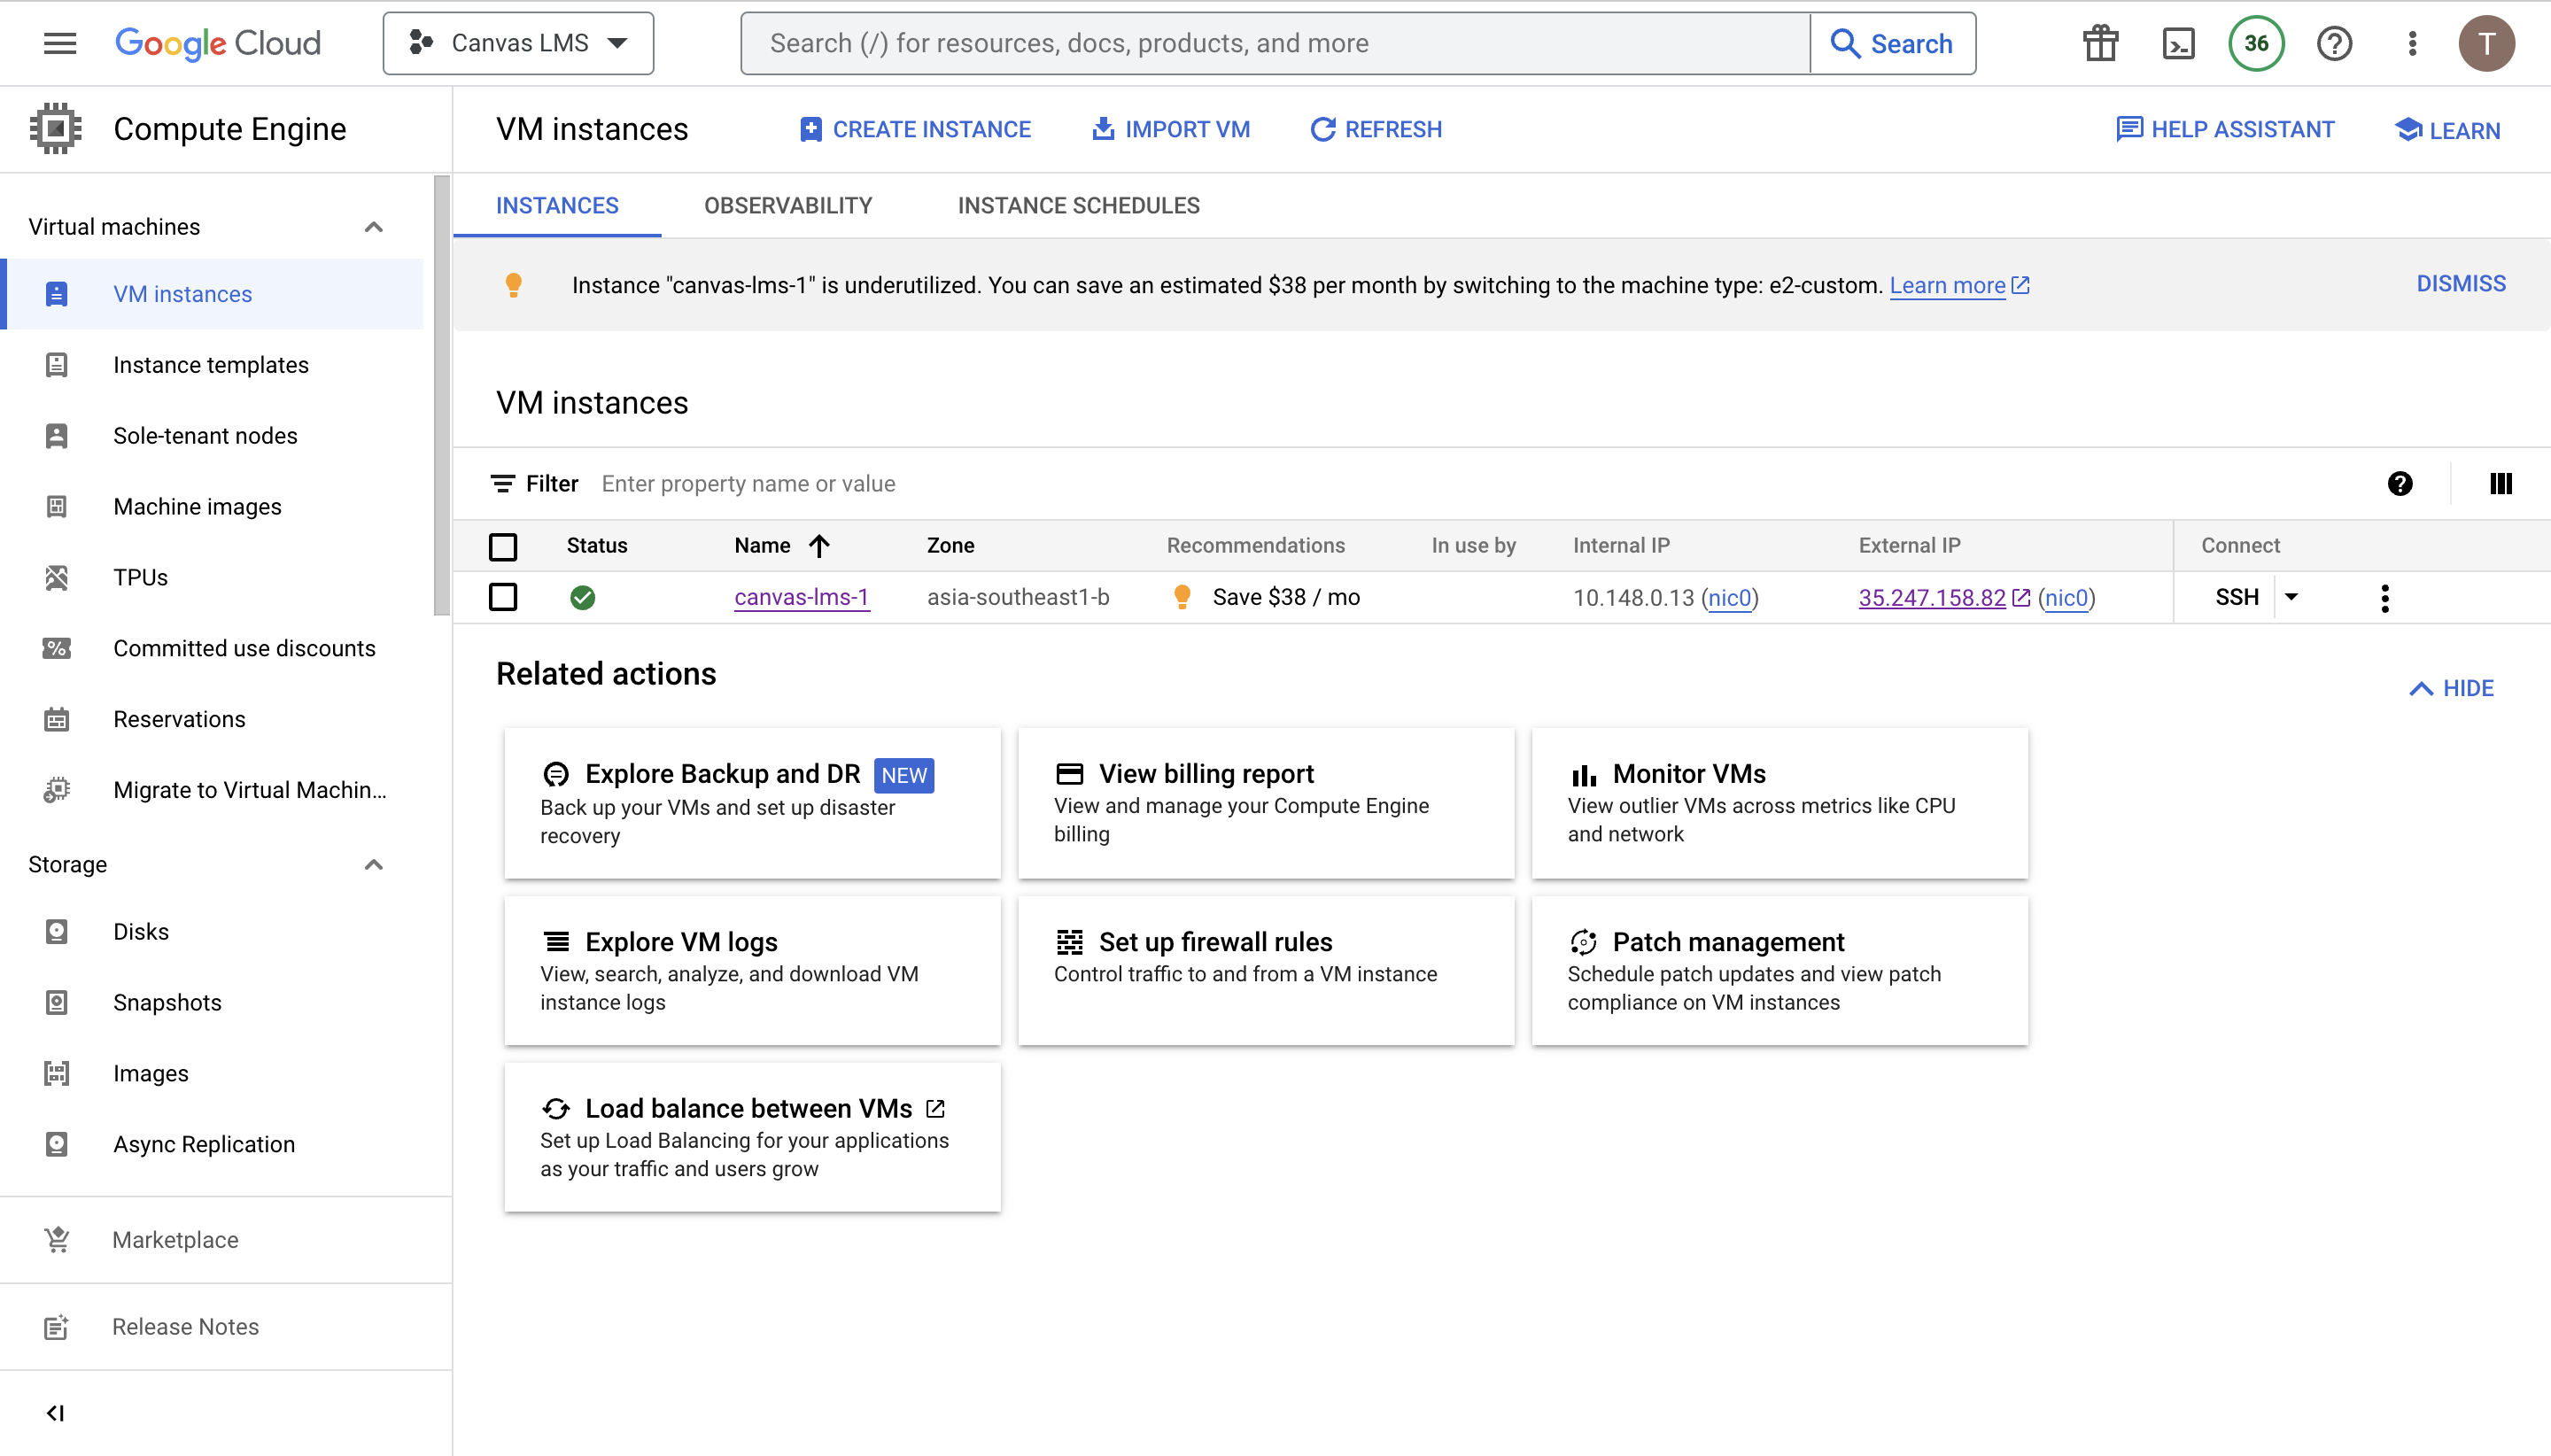
\includegraphics[scale=0.15]{1-google-cloud-console}
            \caption{Màn hình Google Cloud Console}
            \label{fig:google-cloud-console}
        \end{figure}
        \item Tạo máy ảo: Trên bảng điều khiển Google Cloud, chúng ta sẽ thực hiện việc tạo một máy ảo để chạy Canvas LMS. Để tạo máy ảo, chúng ta nhấp vào mục "Compute Engine" trên bảng điều khiển. Tiếp theo, chọn "Máy ảo" và nhấp vào nút "Tạo máy ảo".

        Trong trang tạo máy ảo, bạn sẽ cần cung cấp các thông tin sau:
        \begin{itemize}
            \item Tên máy ảo: Đặt tên cho máy ảo của bạn để dễ nhận biết.
            \item Kích thước máy ảo: Chọn kích thước máy ảo phù hợp với yêu cầu của bạn, bao gồm số lượng bộ nhớ RAM và vCPU.
            \item Vùng địa lý: Chọn vùng địa lý gần với địa điểm của bạn để đảm bảo tốc độ truy cập nhanh nhất.
            \item Firewall: Cấu hình các quy tắc tường lửa cho phép truy cập vào máy ảo.
        \end{itemize}
        \begin{figure}[ht!]
            \centering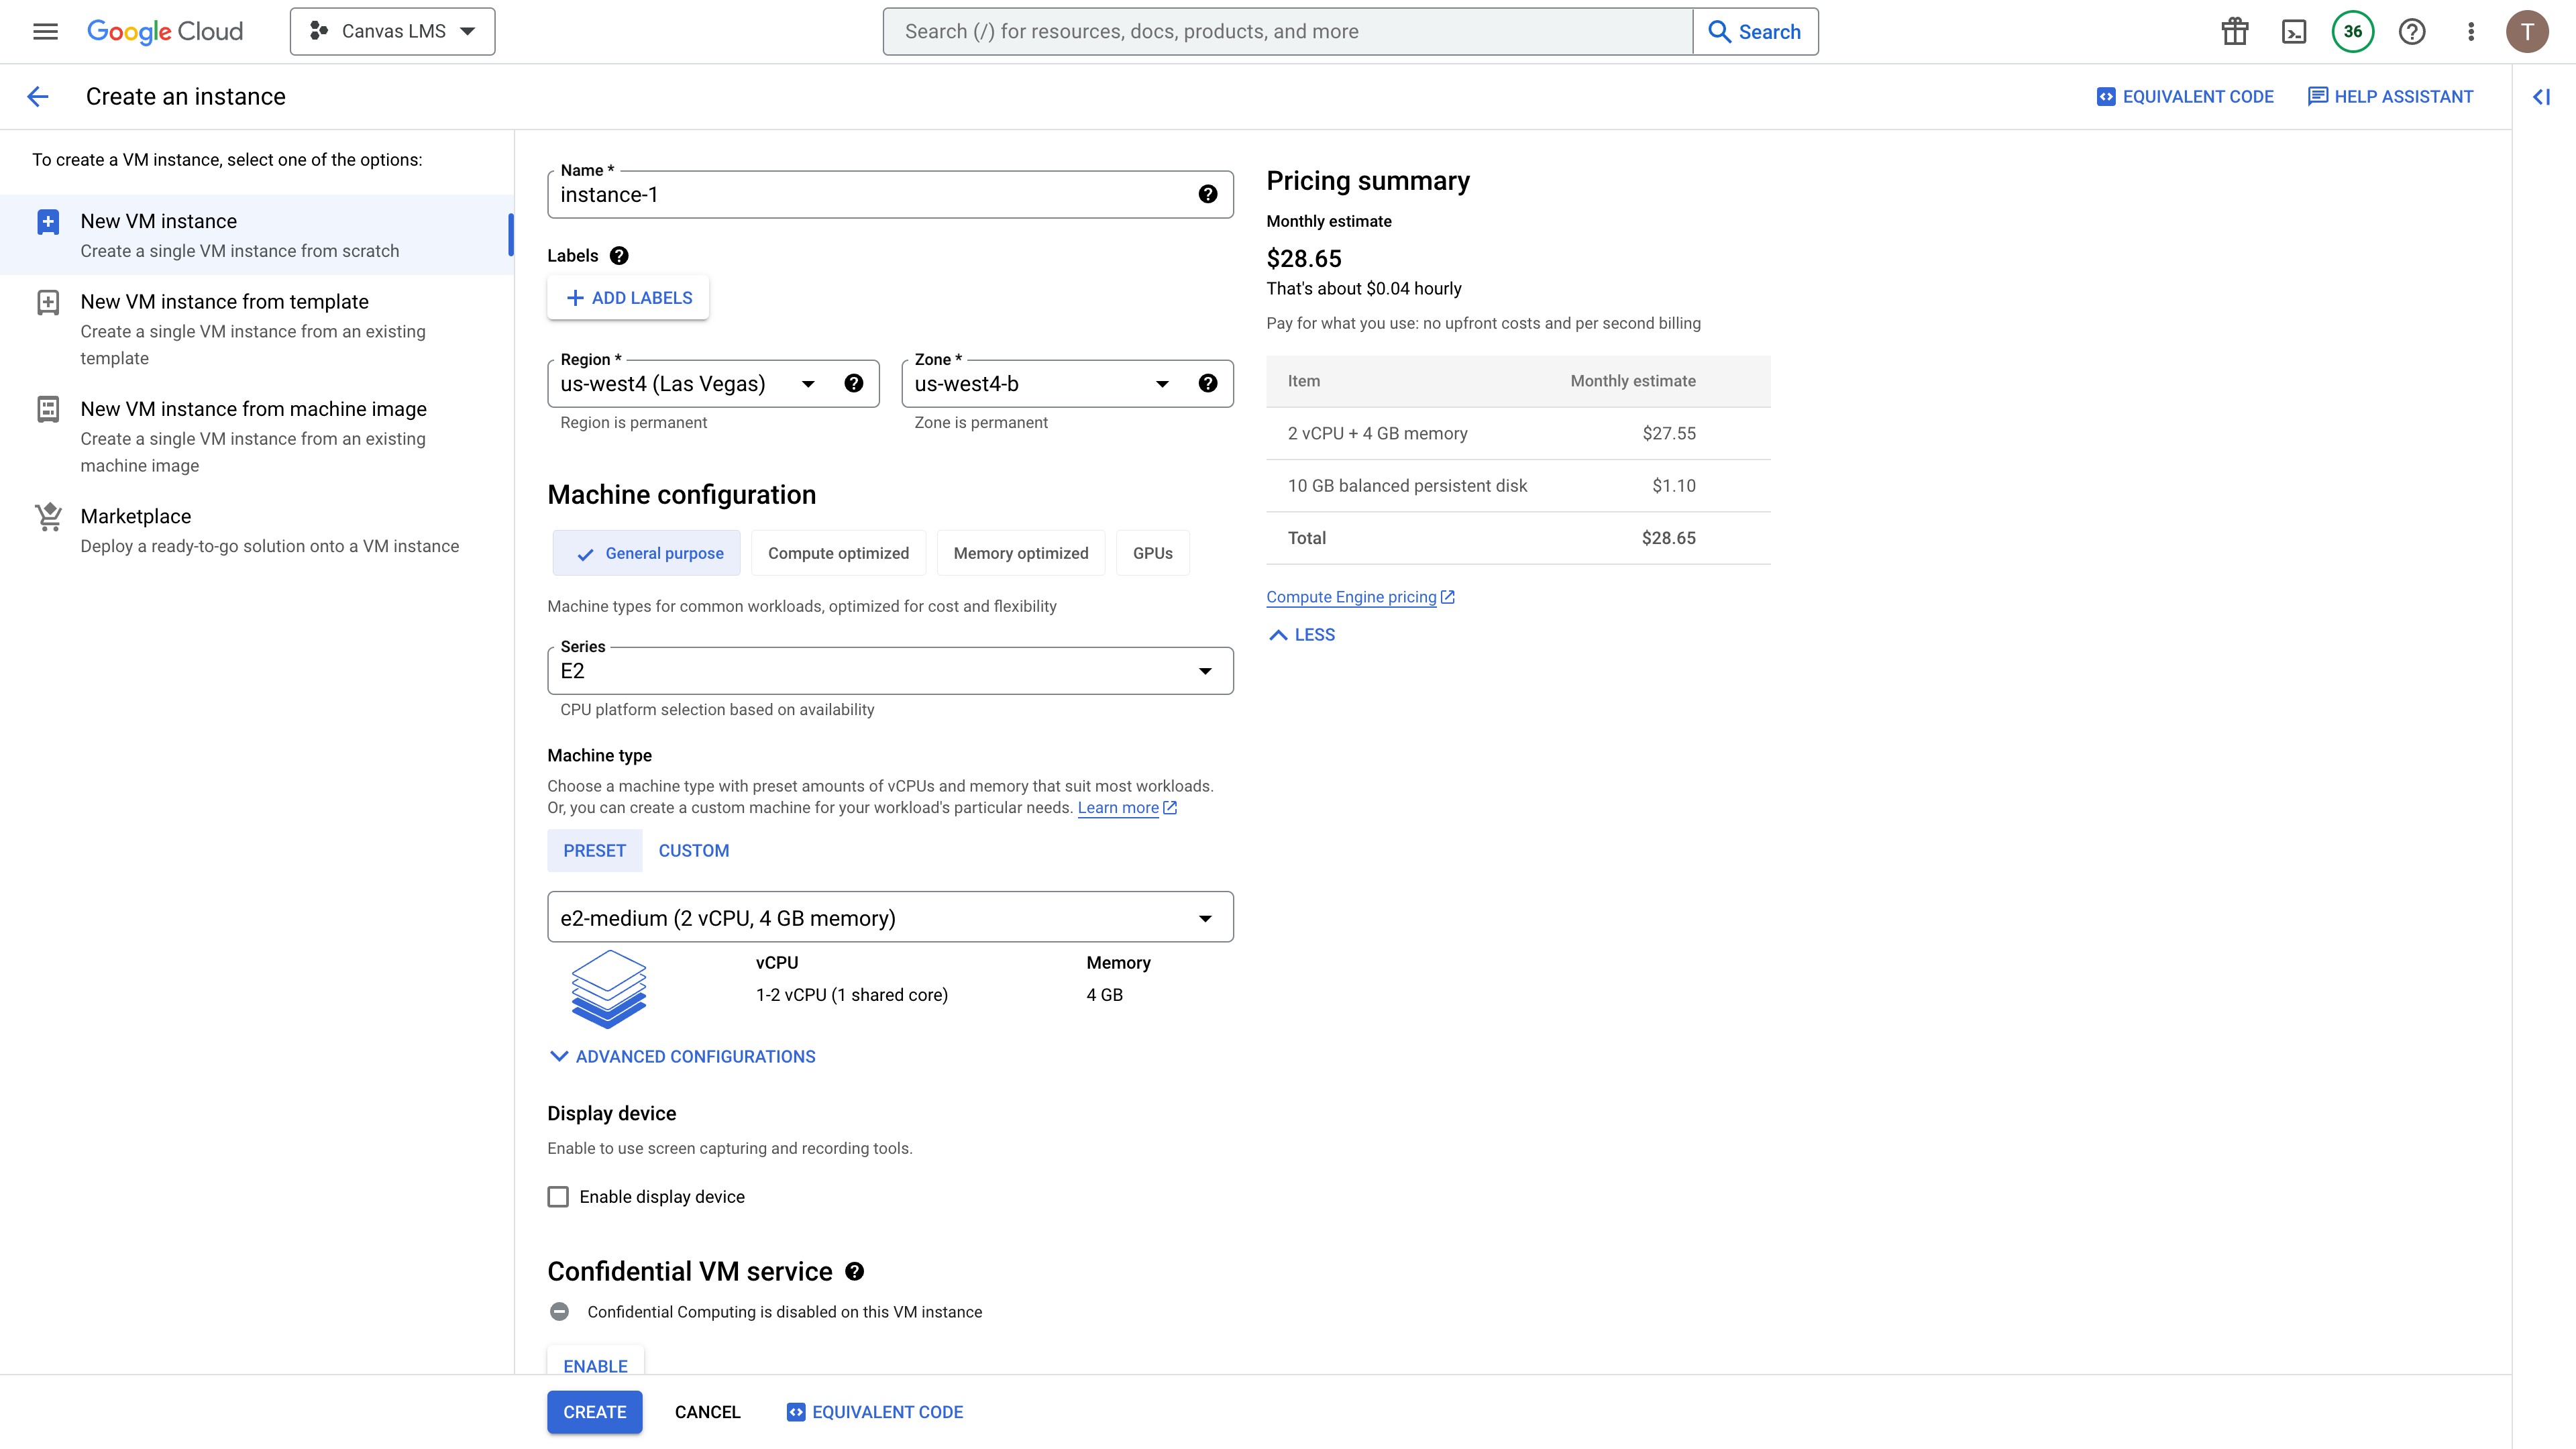
\includegraphics[scale=0.15]{google-create-instance}
            \caption{Màn hình tạo máy ảo}
            \label{fig:google-create-instance}
        \end{figure}

        \item Cấu hình mạng: Đảm bảo rằng máy ảo của bạn được cấu hình để có địa chỉ IP công cộng và có quyền truy cập Internet. Điều này sẽ đảm bảo rằng máy ảo có thể truy cập vào các tài nguyên cần thiết và có thể phục vụ các yêu cầu từ người dùng.

        Trên bảng điều khiển Google Cloud, chúng ta có thể cấu hình các thiết lập mạng cho máy ảo bằng cách điều hướng đến mục "Network" hoặc "Mạng" trên bảng điều khiển.
        
        Ở đây, chúng ta có thể thực hiện các tác vụ như gán địa chỉ IP công cộng, tạo và quản lý các quy tắc tường lửa, cấu hình phân giải tên miền và nhiều hơn nữa.

        \begin{figure}[ht!]
            \centering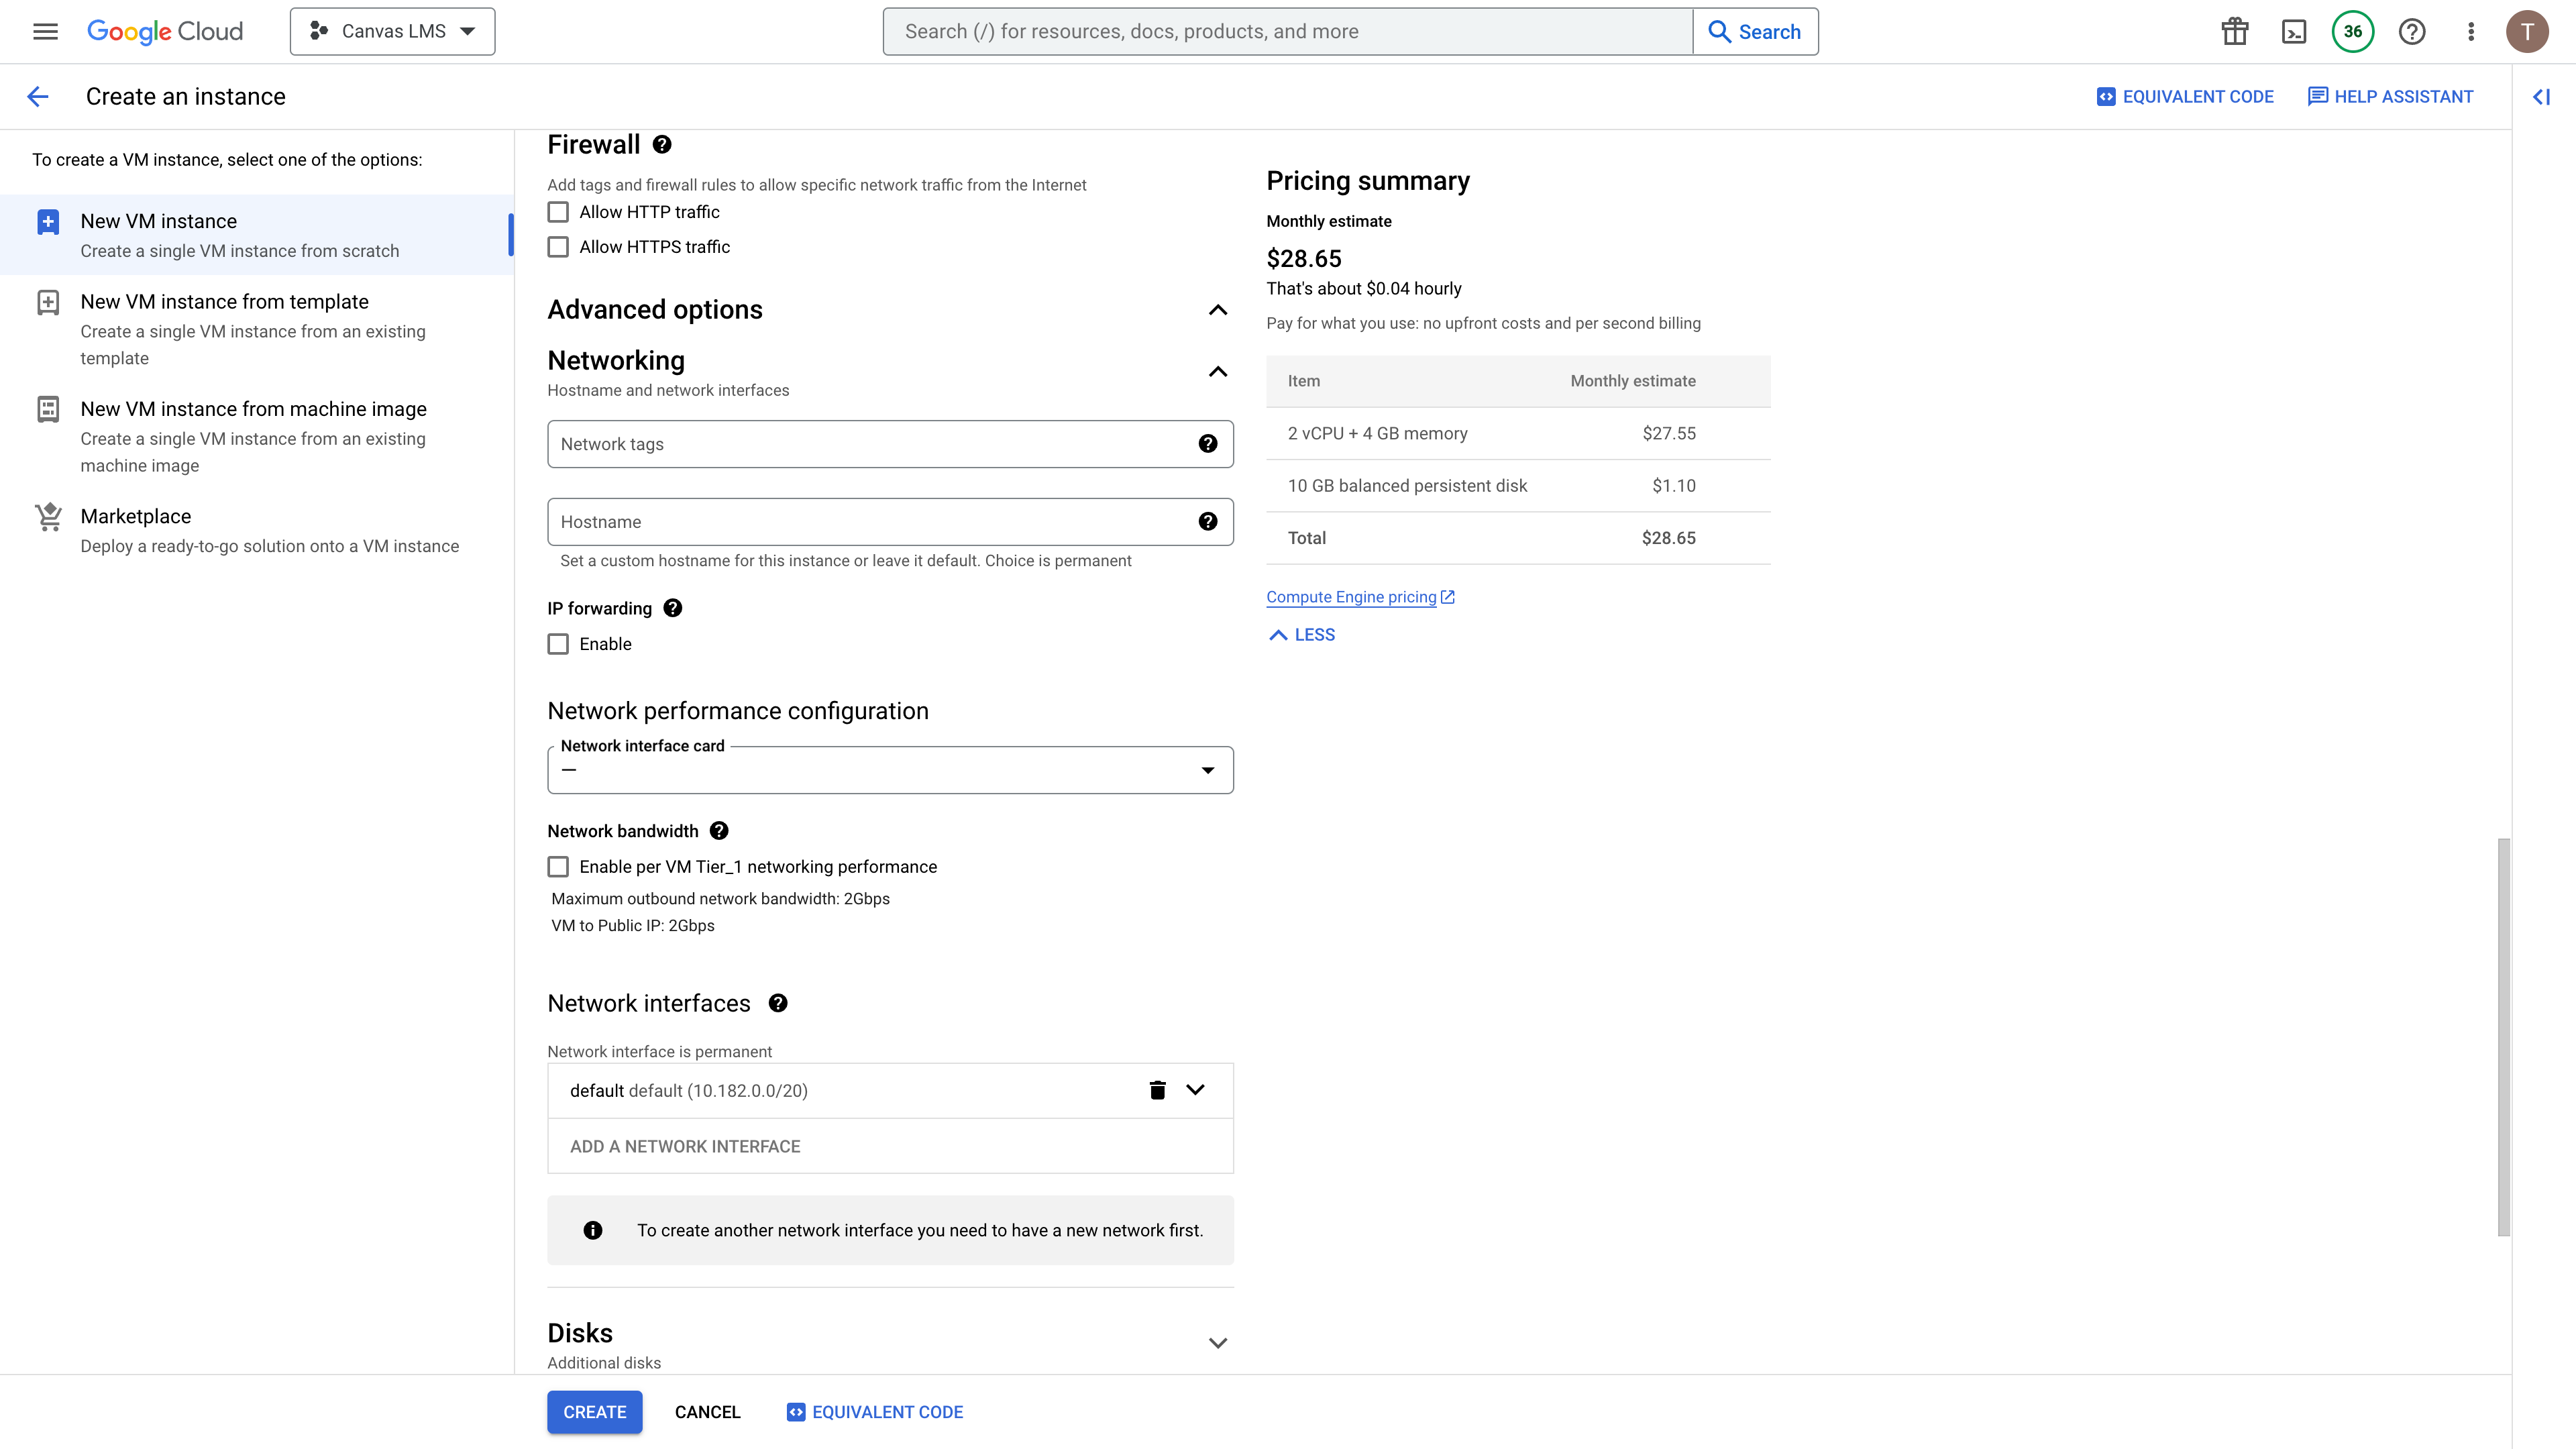
\includegraphics[scale=0.15]{google-network}
            \caption{Cài đặt mạng cho máy ảo}
            \label{fig:google-network}
        \end{figure}

        \item Cài đặt và cấu hình Canvas LMS: Sau khi đã chuẩn bị môi trường, chúng ta có thể tiến hành cài đặt và cấu hình Canvas LMS trên máy ảo. Quá trình này bao gồm cài đặt Ruby, PostgreSQL, các gói phụ thuộc và mã nguồn Canvas LMS.

        Để cài đặt và cấu hình Canvas LMS, chúng ta sẽ sử dụng các lệnh và tệp cấu hình được cung cấp trong mã nguồn của Canvas LMS. Quá trình này yêu cầu kiến thức về quản lý máy chủ và cài đặt ứng dụng web.
        
        Sau khi cài đặt và cấu hình thành công, chúng ta sẽ có một môi trường Canvas LMS hoạt động trên máy ảo của chúng ta trên Google Cloud.
    \end{enumerate}
    \subsection{Cài đặt Canvas LMS}
    \subsection{Kiểm tra và triển khai}
    \subsection{Cài đặt và cấu hình các thành phần hỗ trợ}

    \begin{figure}[ht!]
        \centering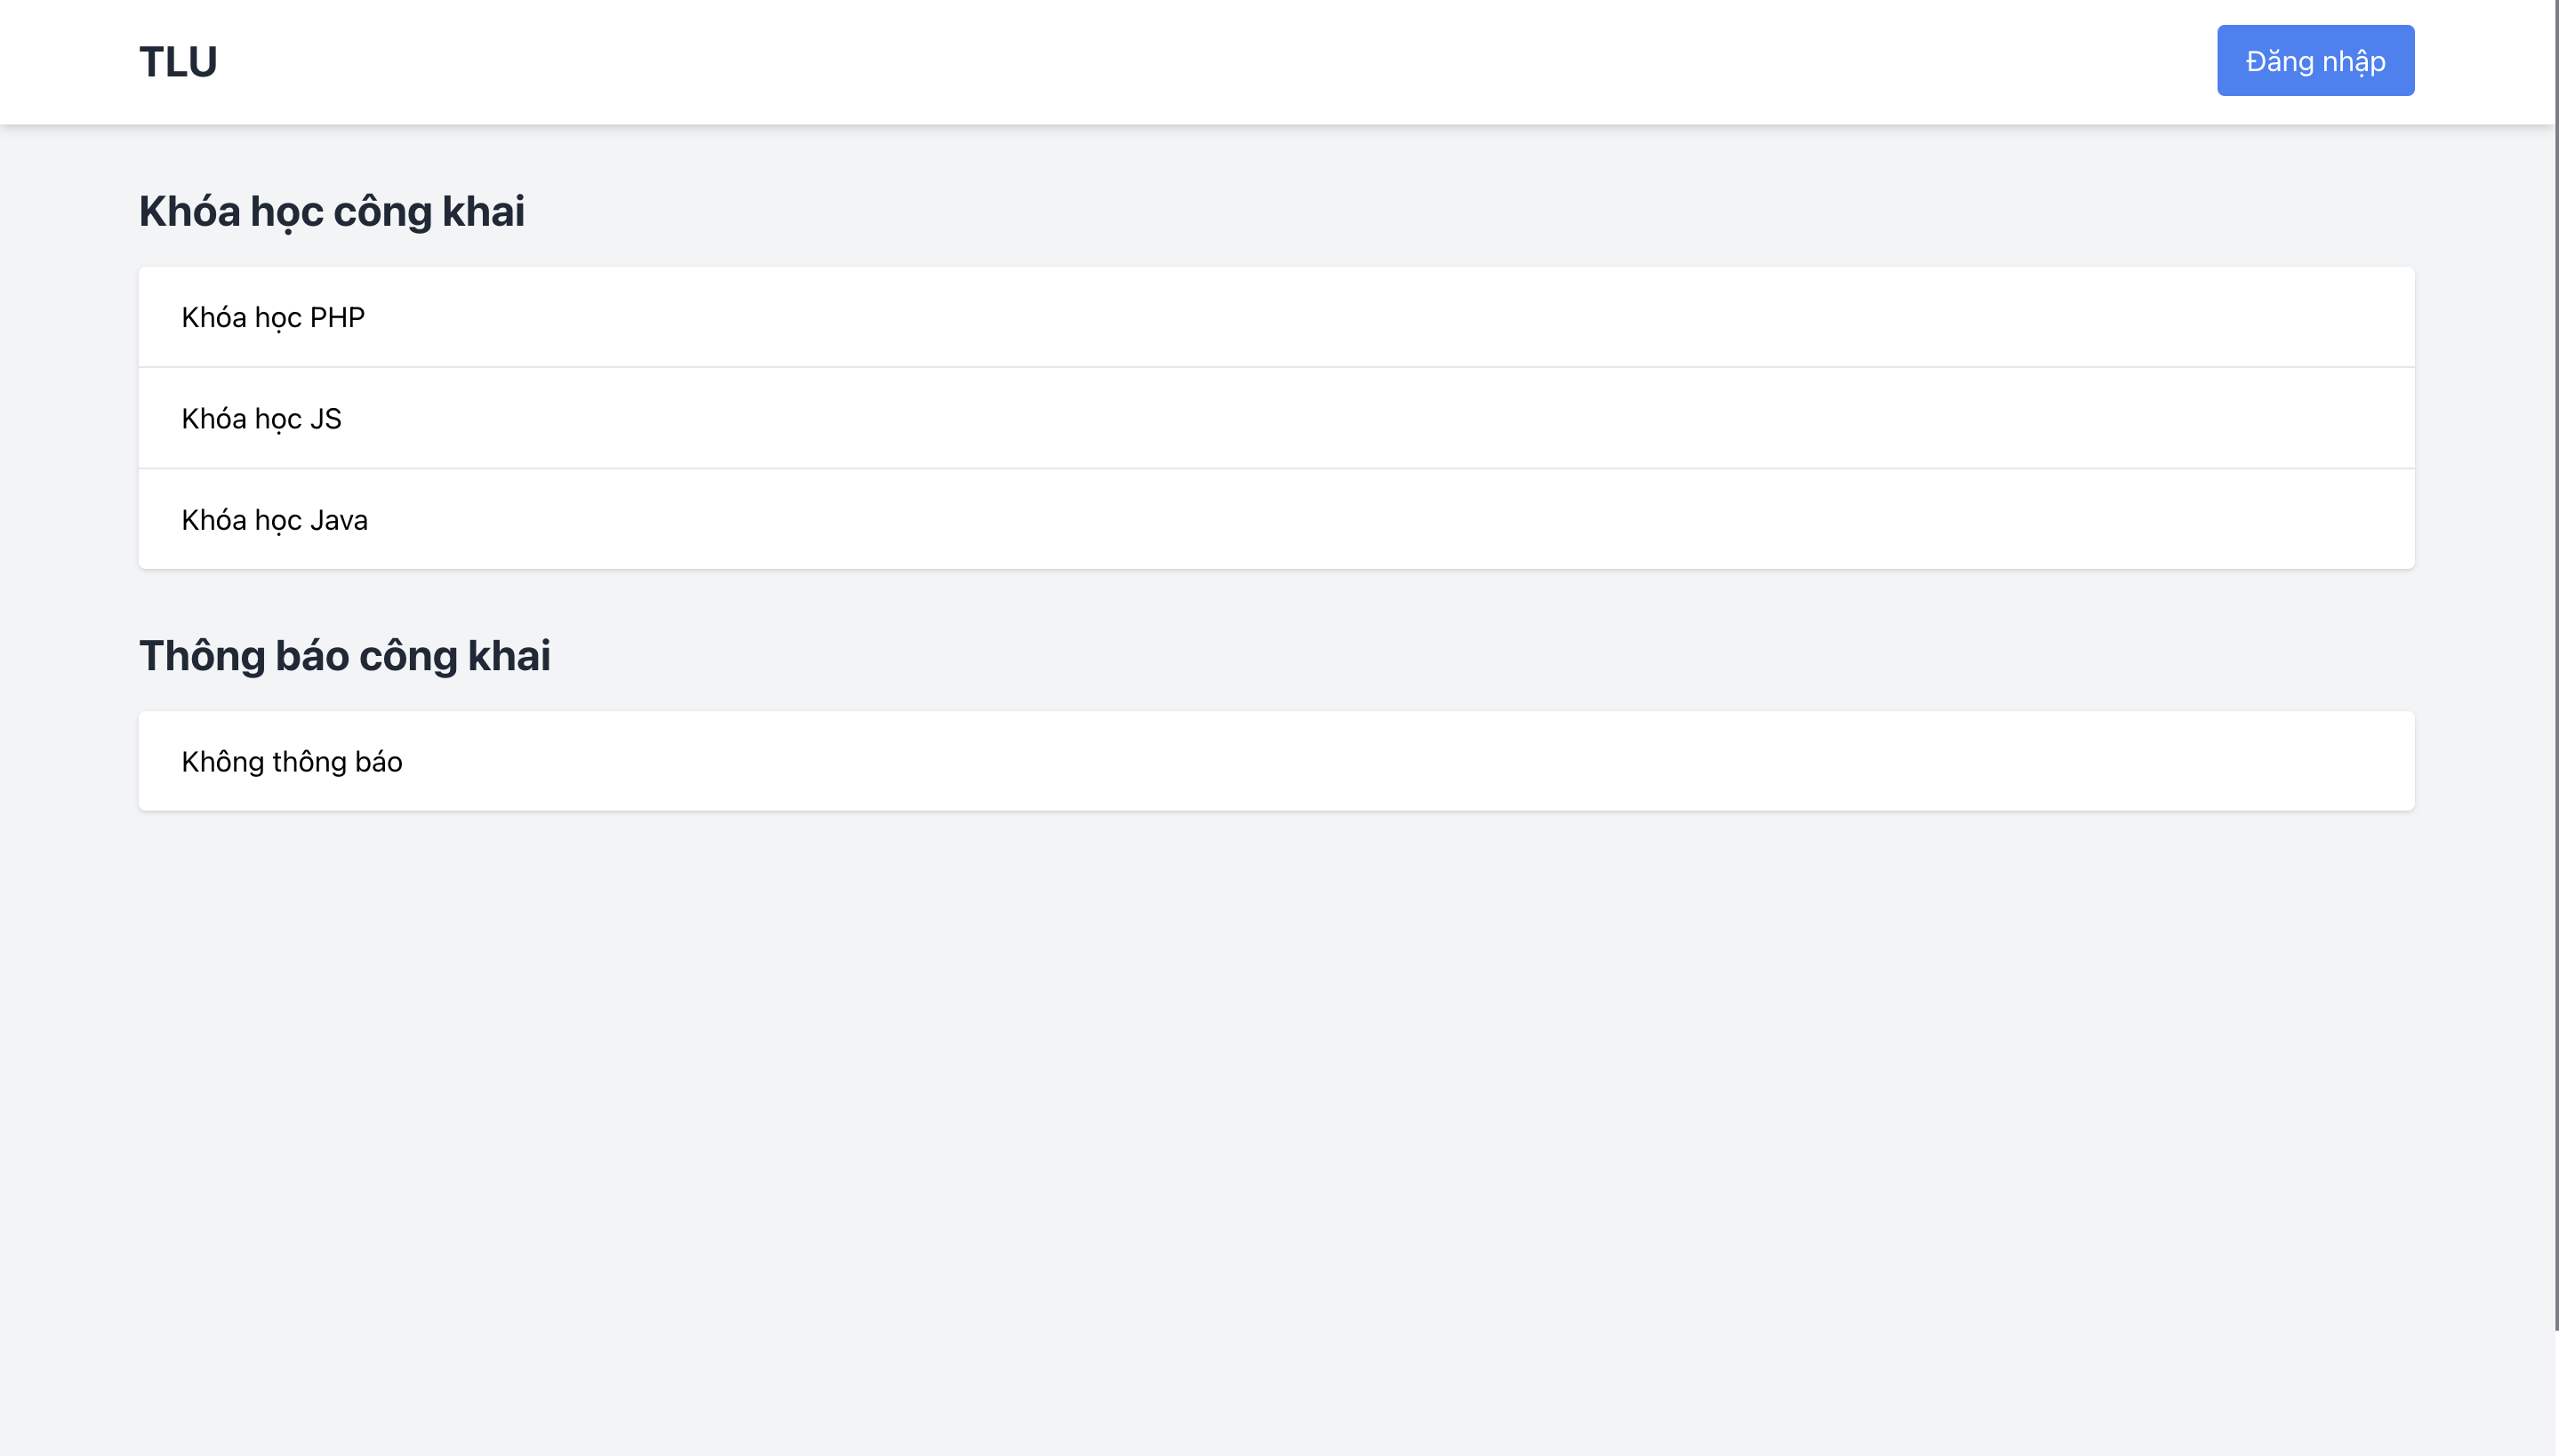
\includegraphics[scale=0.15]{2-landing-page}
        \caption{Màn hình Landing Page}
        \label{fig:landing-page}
    \end{figure}

    \begin{figure}[ht!]
        \centering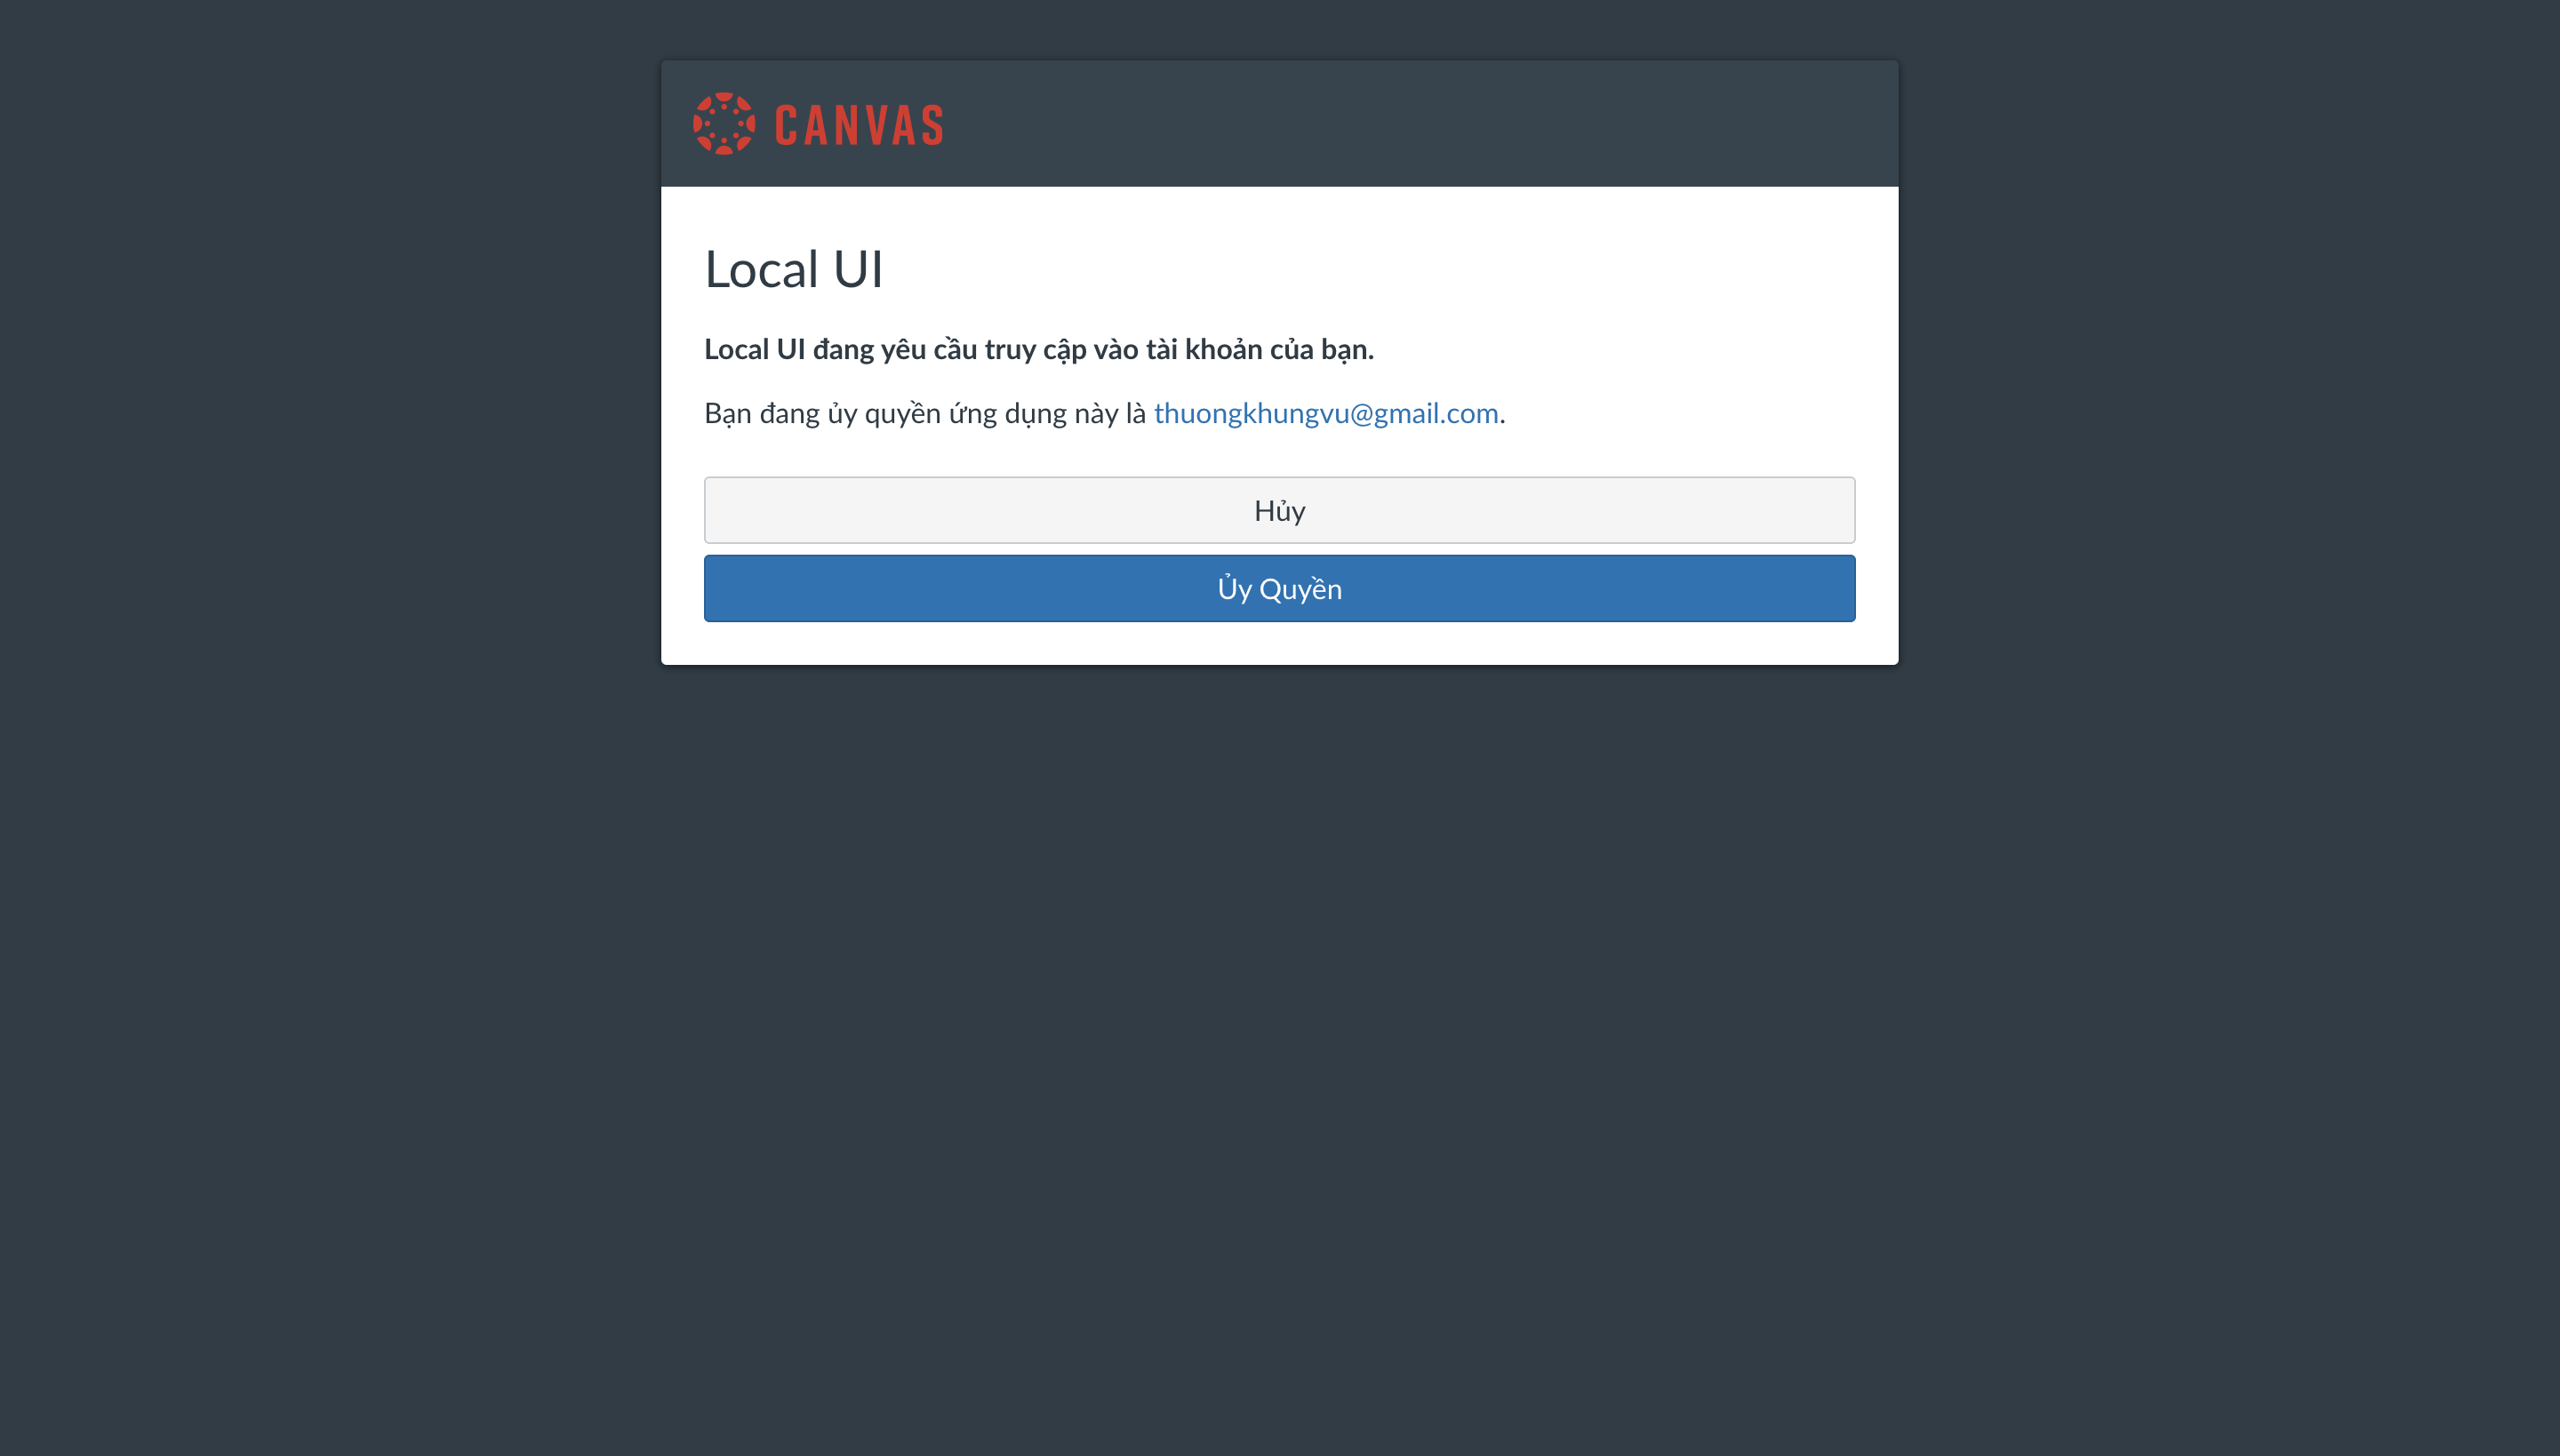
\includegraphics[scale=0.15]{3-dang-nhap}
        \caption{Màn hình Login Page}
        \label{fig:dang-nhap}
    \end{figure}

    \begin{figure}[ht!]
        \centering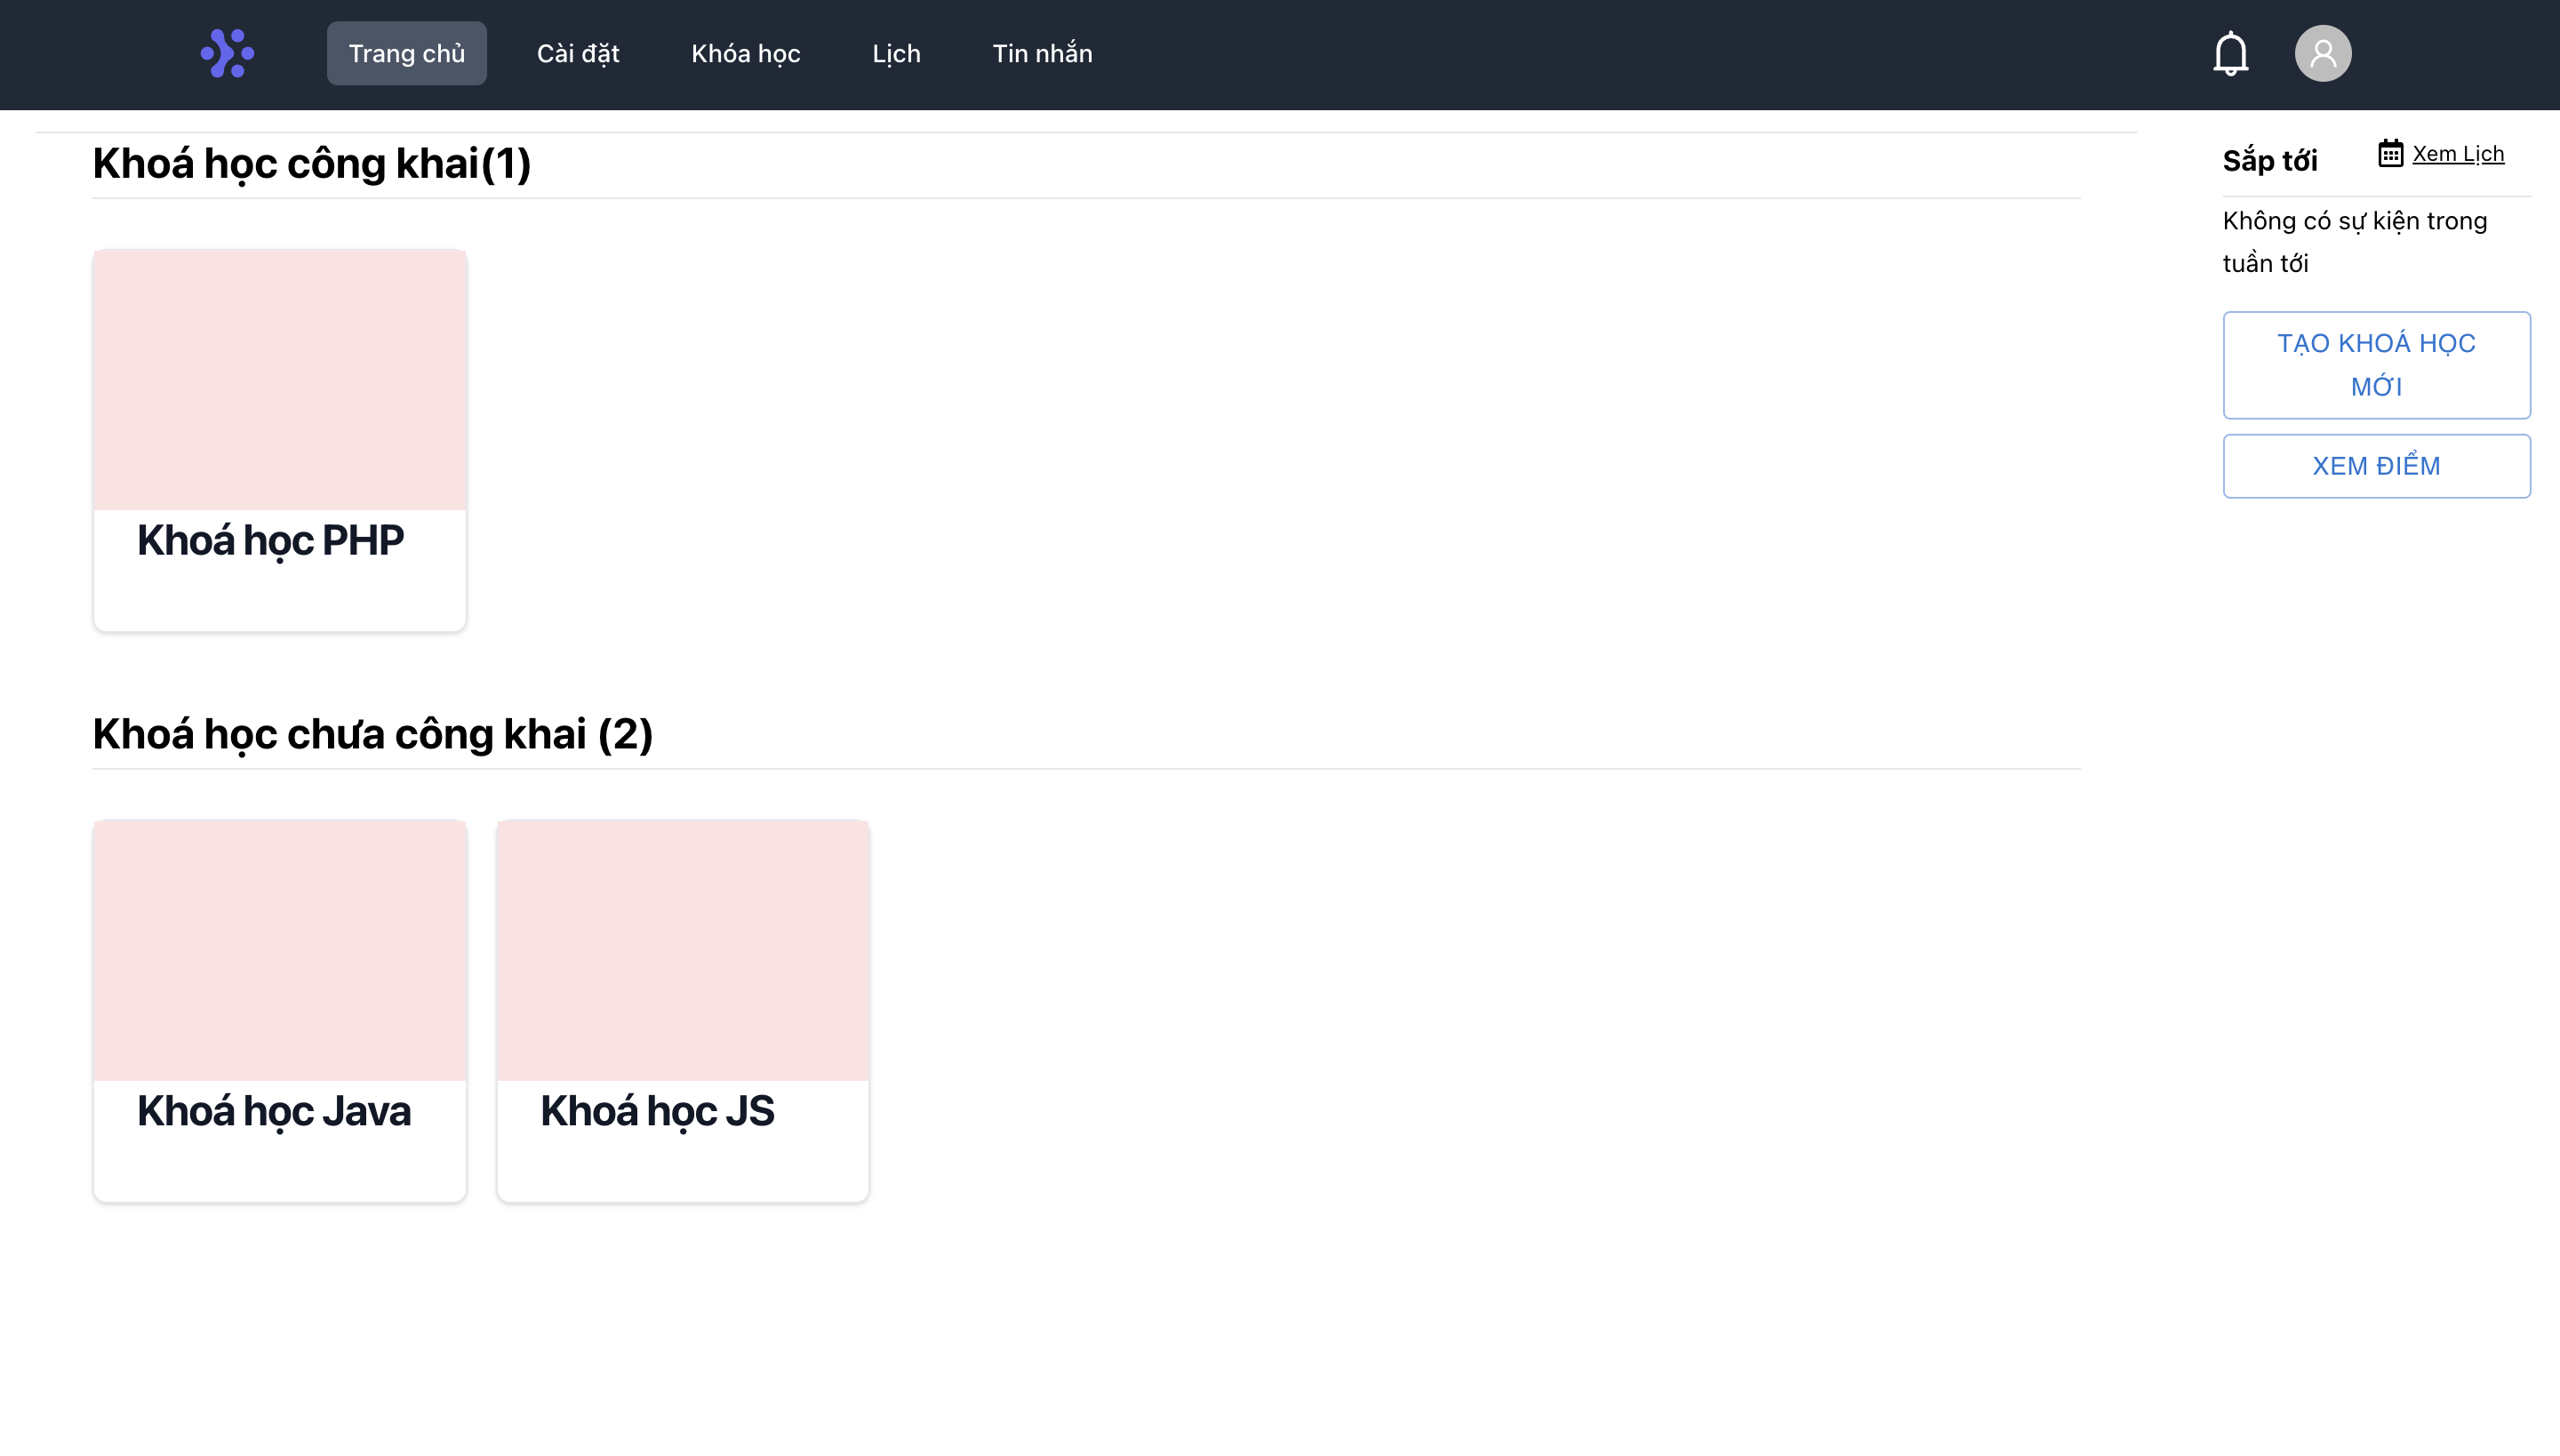
\includegraphics[scale=0.15]{4-trang-chu}
        \caption{Màn hình Home Page}
        \label{fig:trang-chu}
    \end{figure}

    \begin{figure}[ht!]
        \centering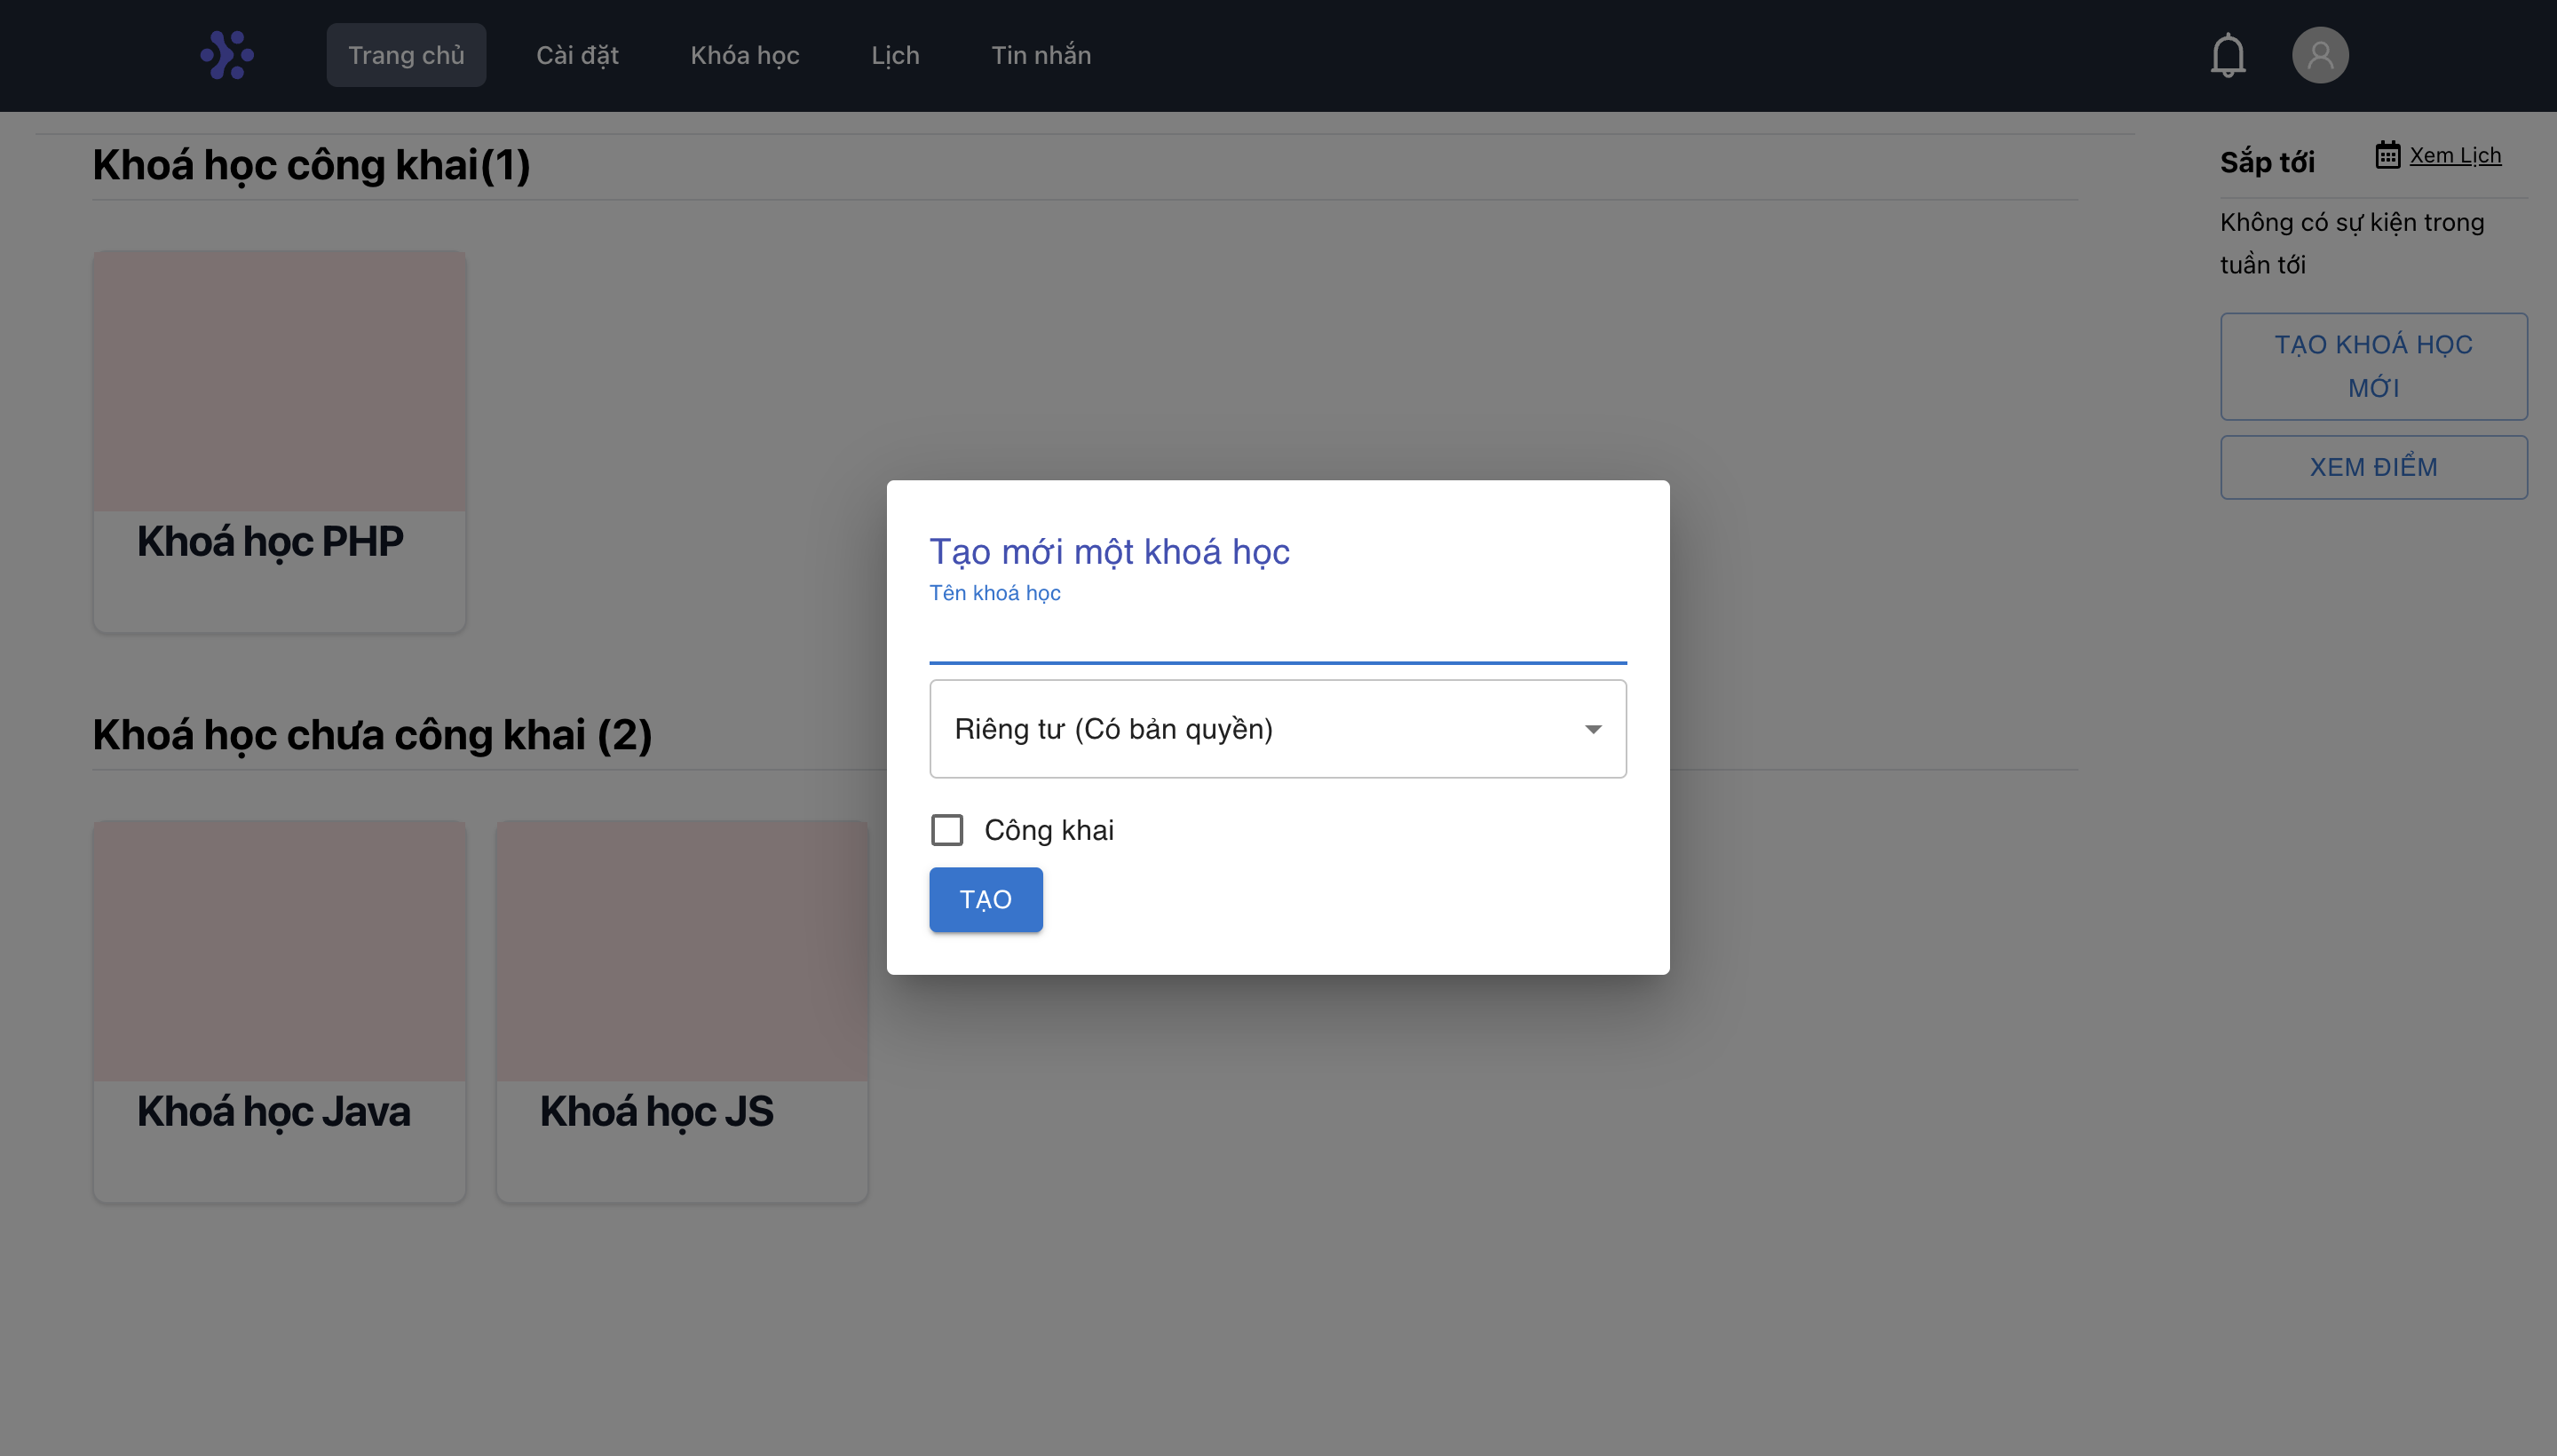
\includegraphics[scale=0.15]{5-tao-khoa-hoc}
        \caption{Màn hình Tạo khoá học}
        \label{fig:tao-khoa-hoc}
    \end{figure}
    \begin{figure}[ht!]
        \centering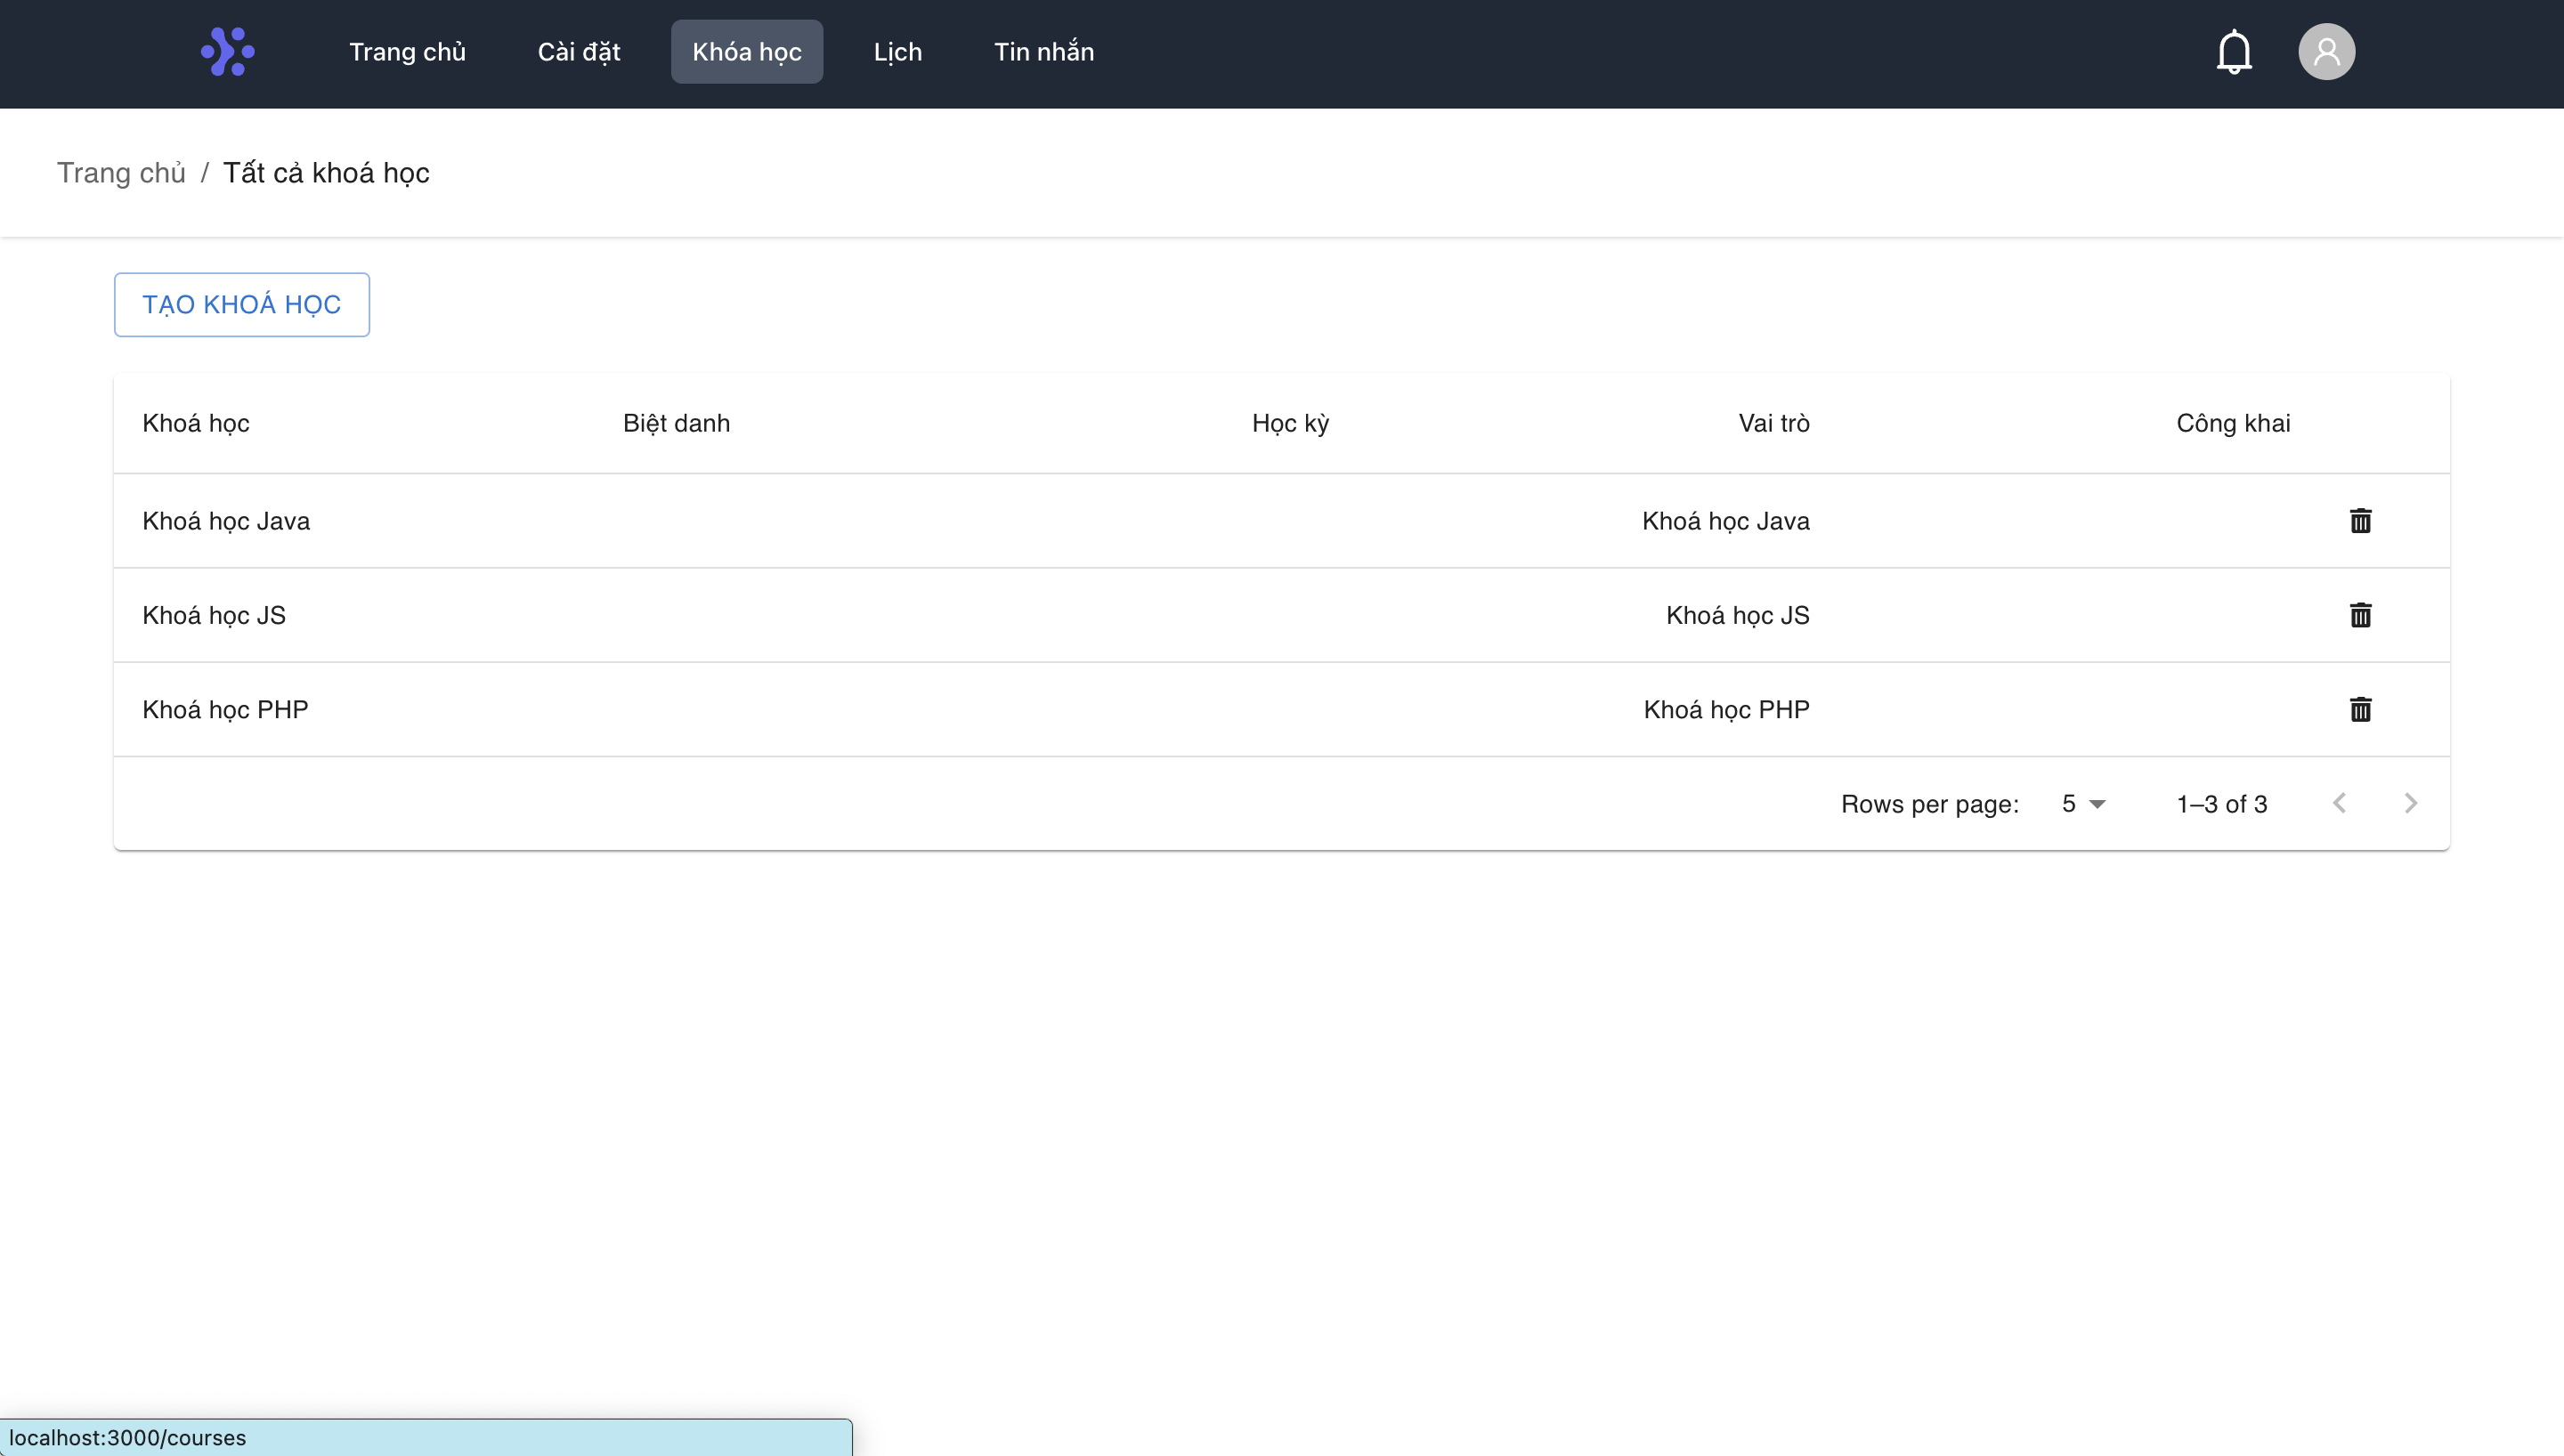
\includegraphics[scale=0.15]{6-danh-sach-khoa-hoc}
        \caption{Màn hình Danh sách khóa học}
        \label{fig:danh-sach-khoa-hoc}
    \end{figure}
    
    \begin{figure}[ht!]
        \centering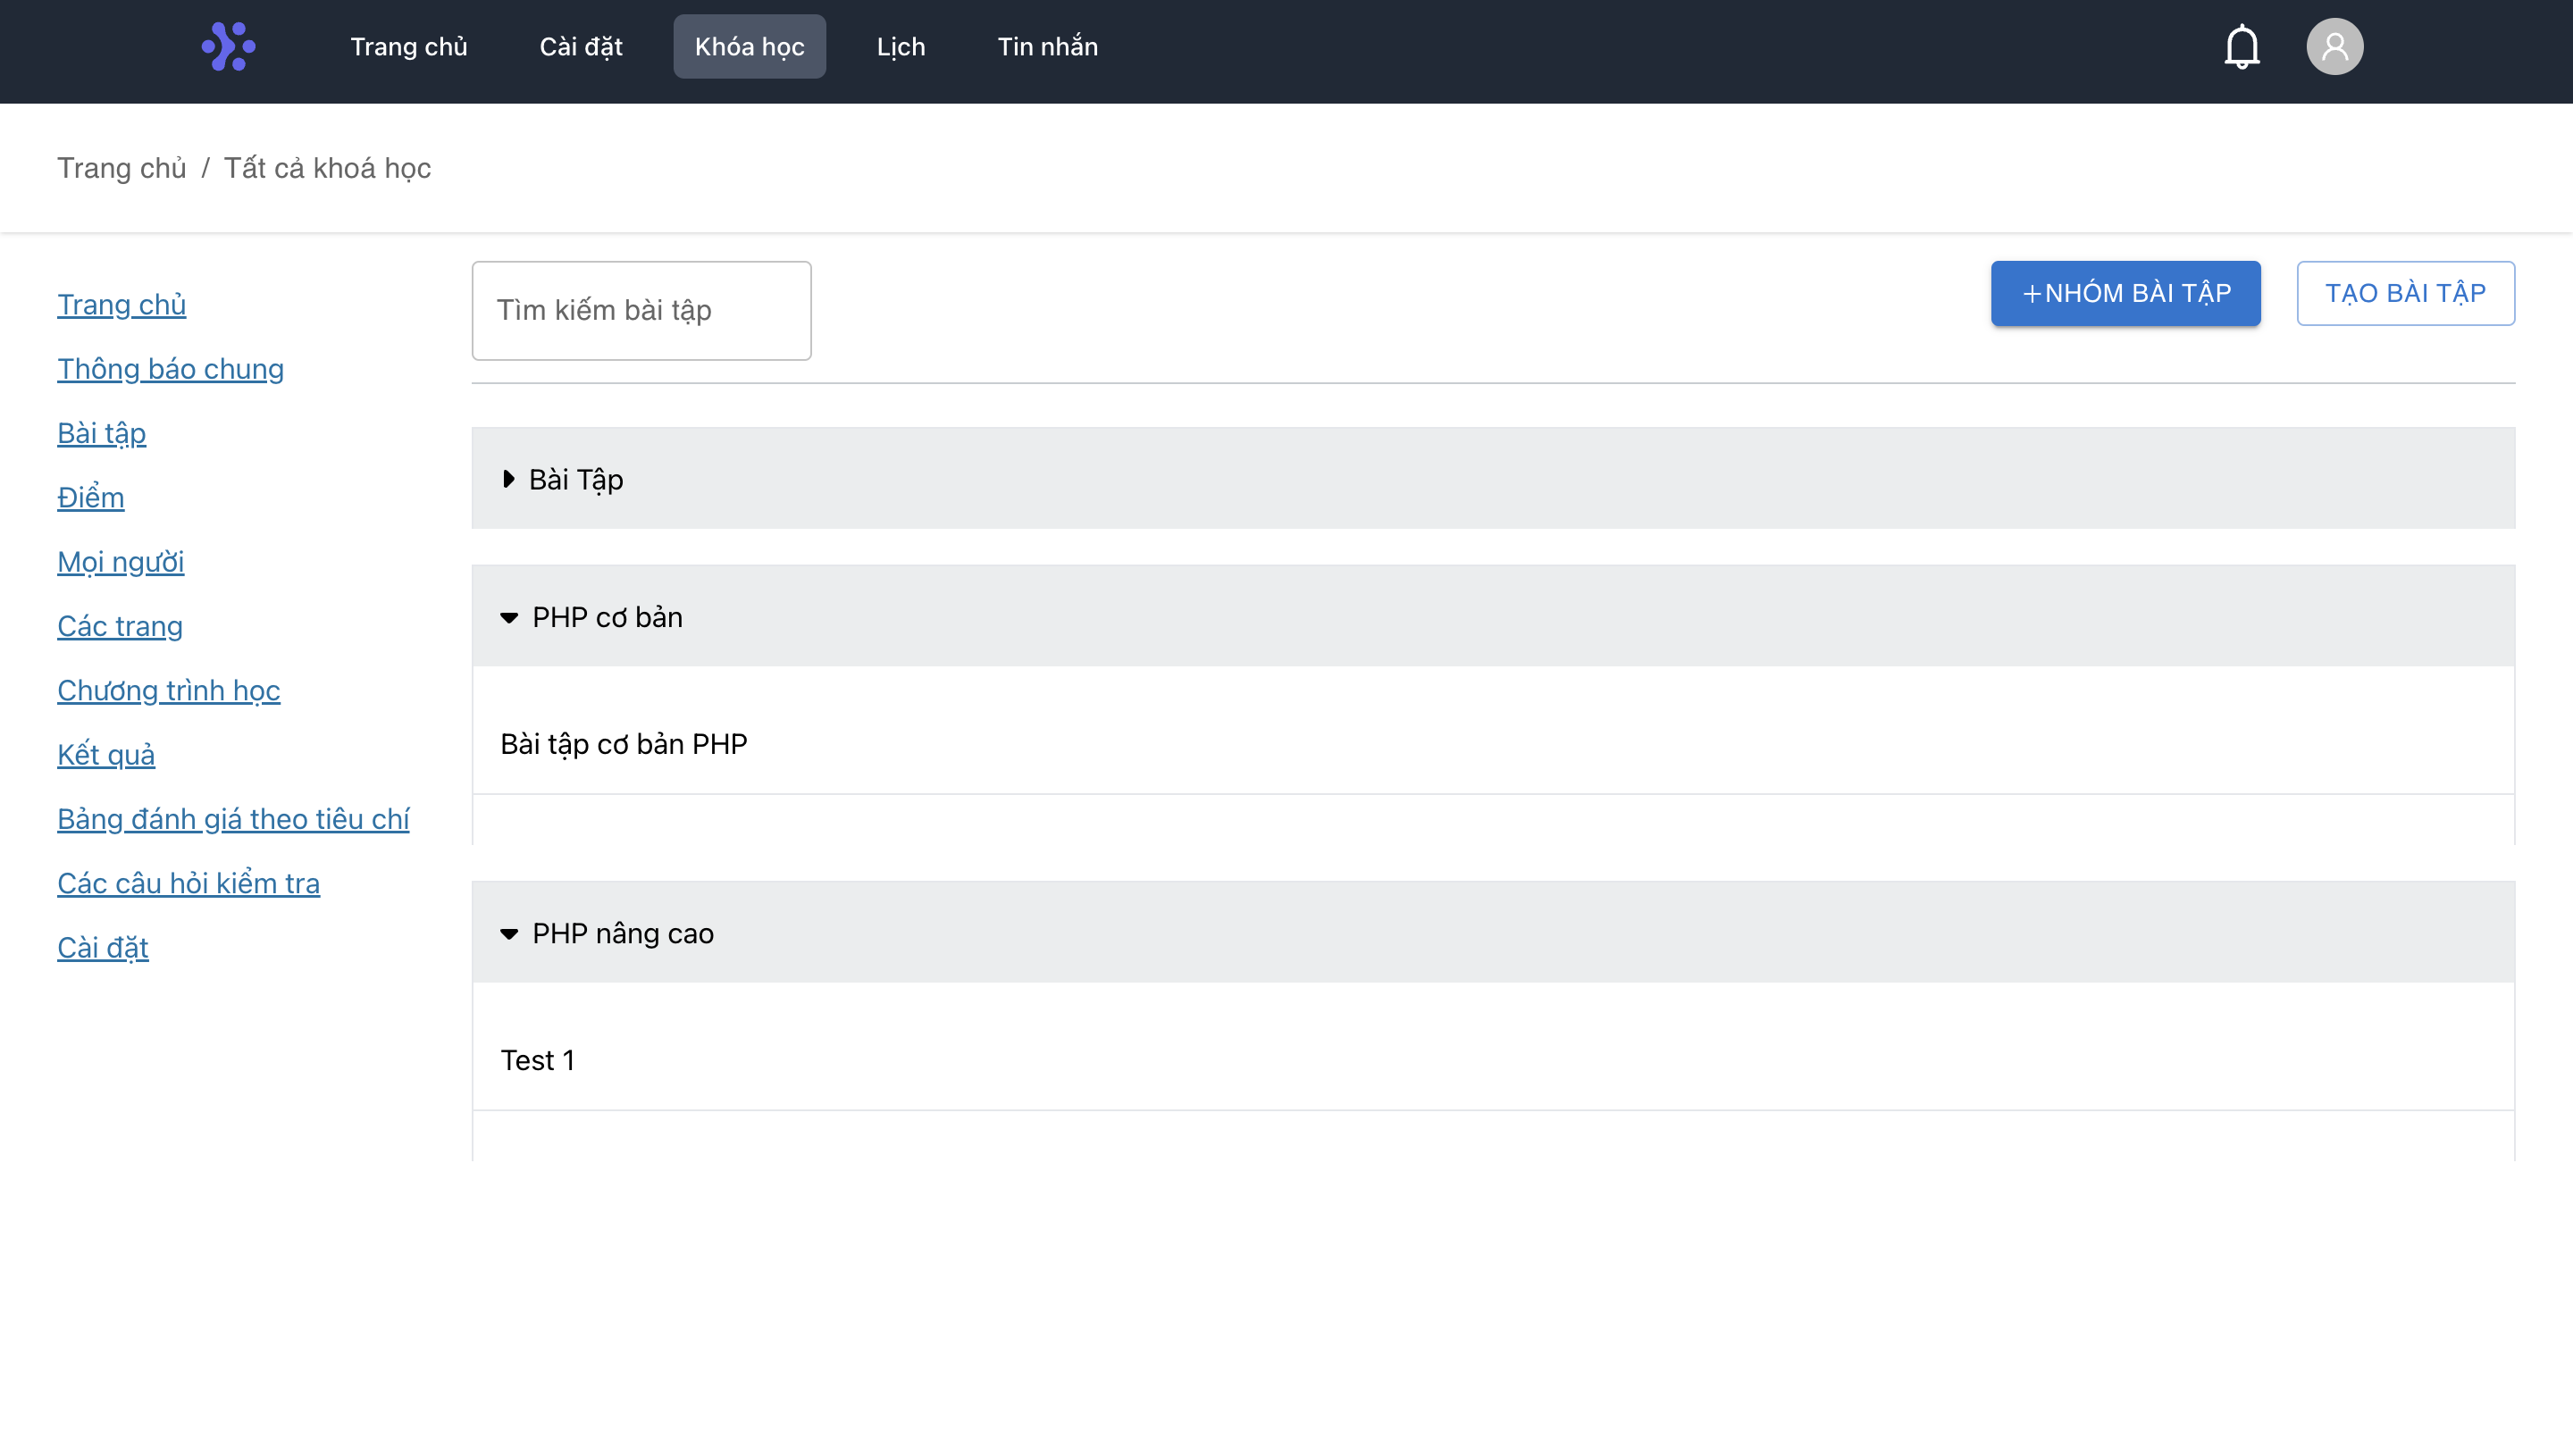
\includegraphics[scale=0.15]{7-danh-sach-nhom-va-bai-tap}
        \caption{Màn hình Danh sách nhóm và bài tập}
        \label{fig:danh-sach-group-va-bai-tap}
    \end{figure}


    \begin{figure}[ht!]
        \centering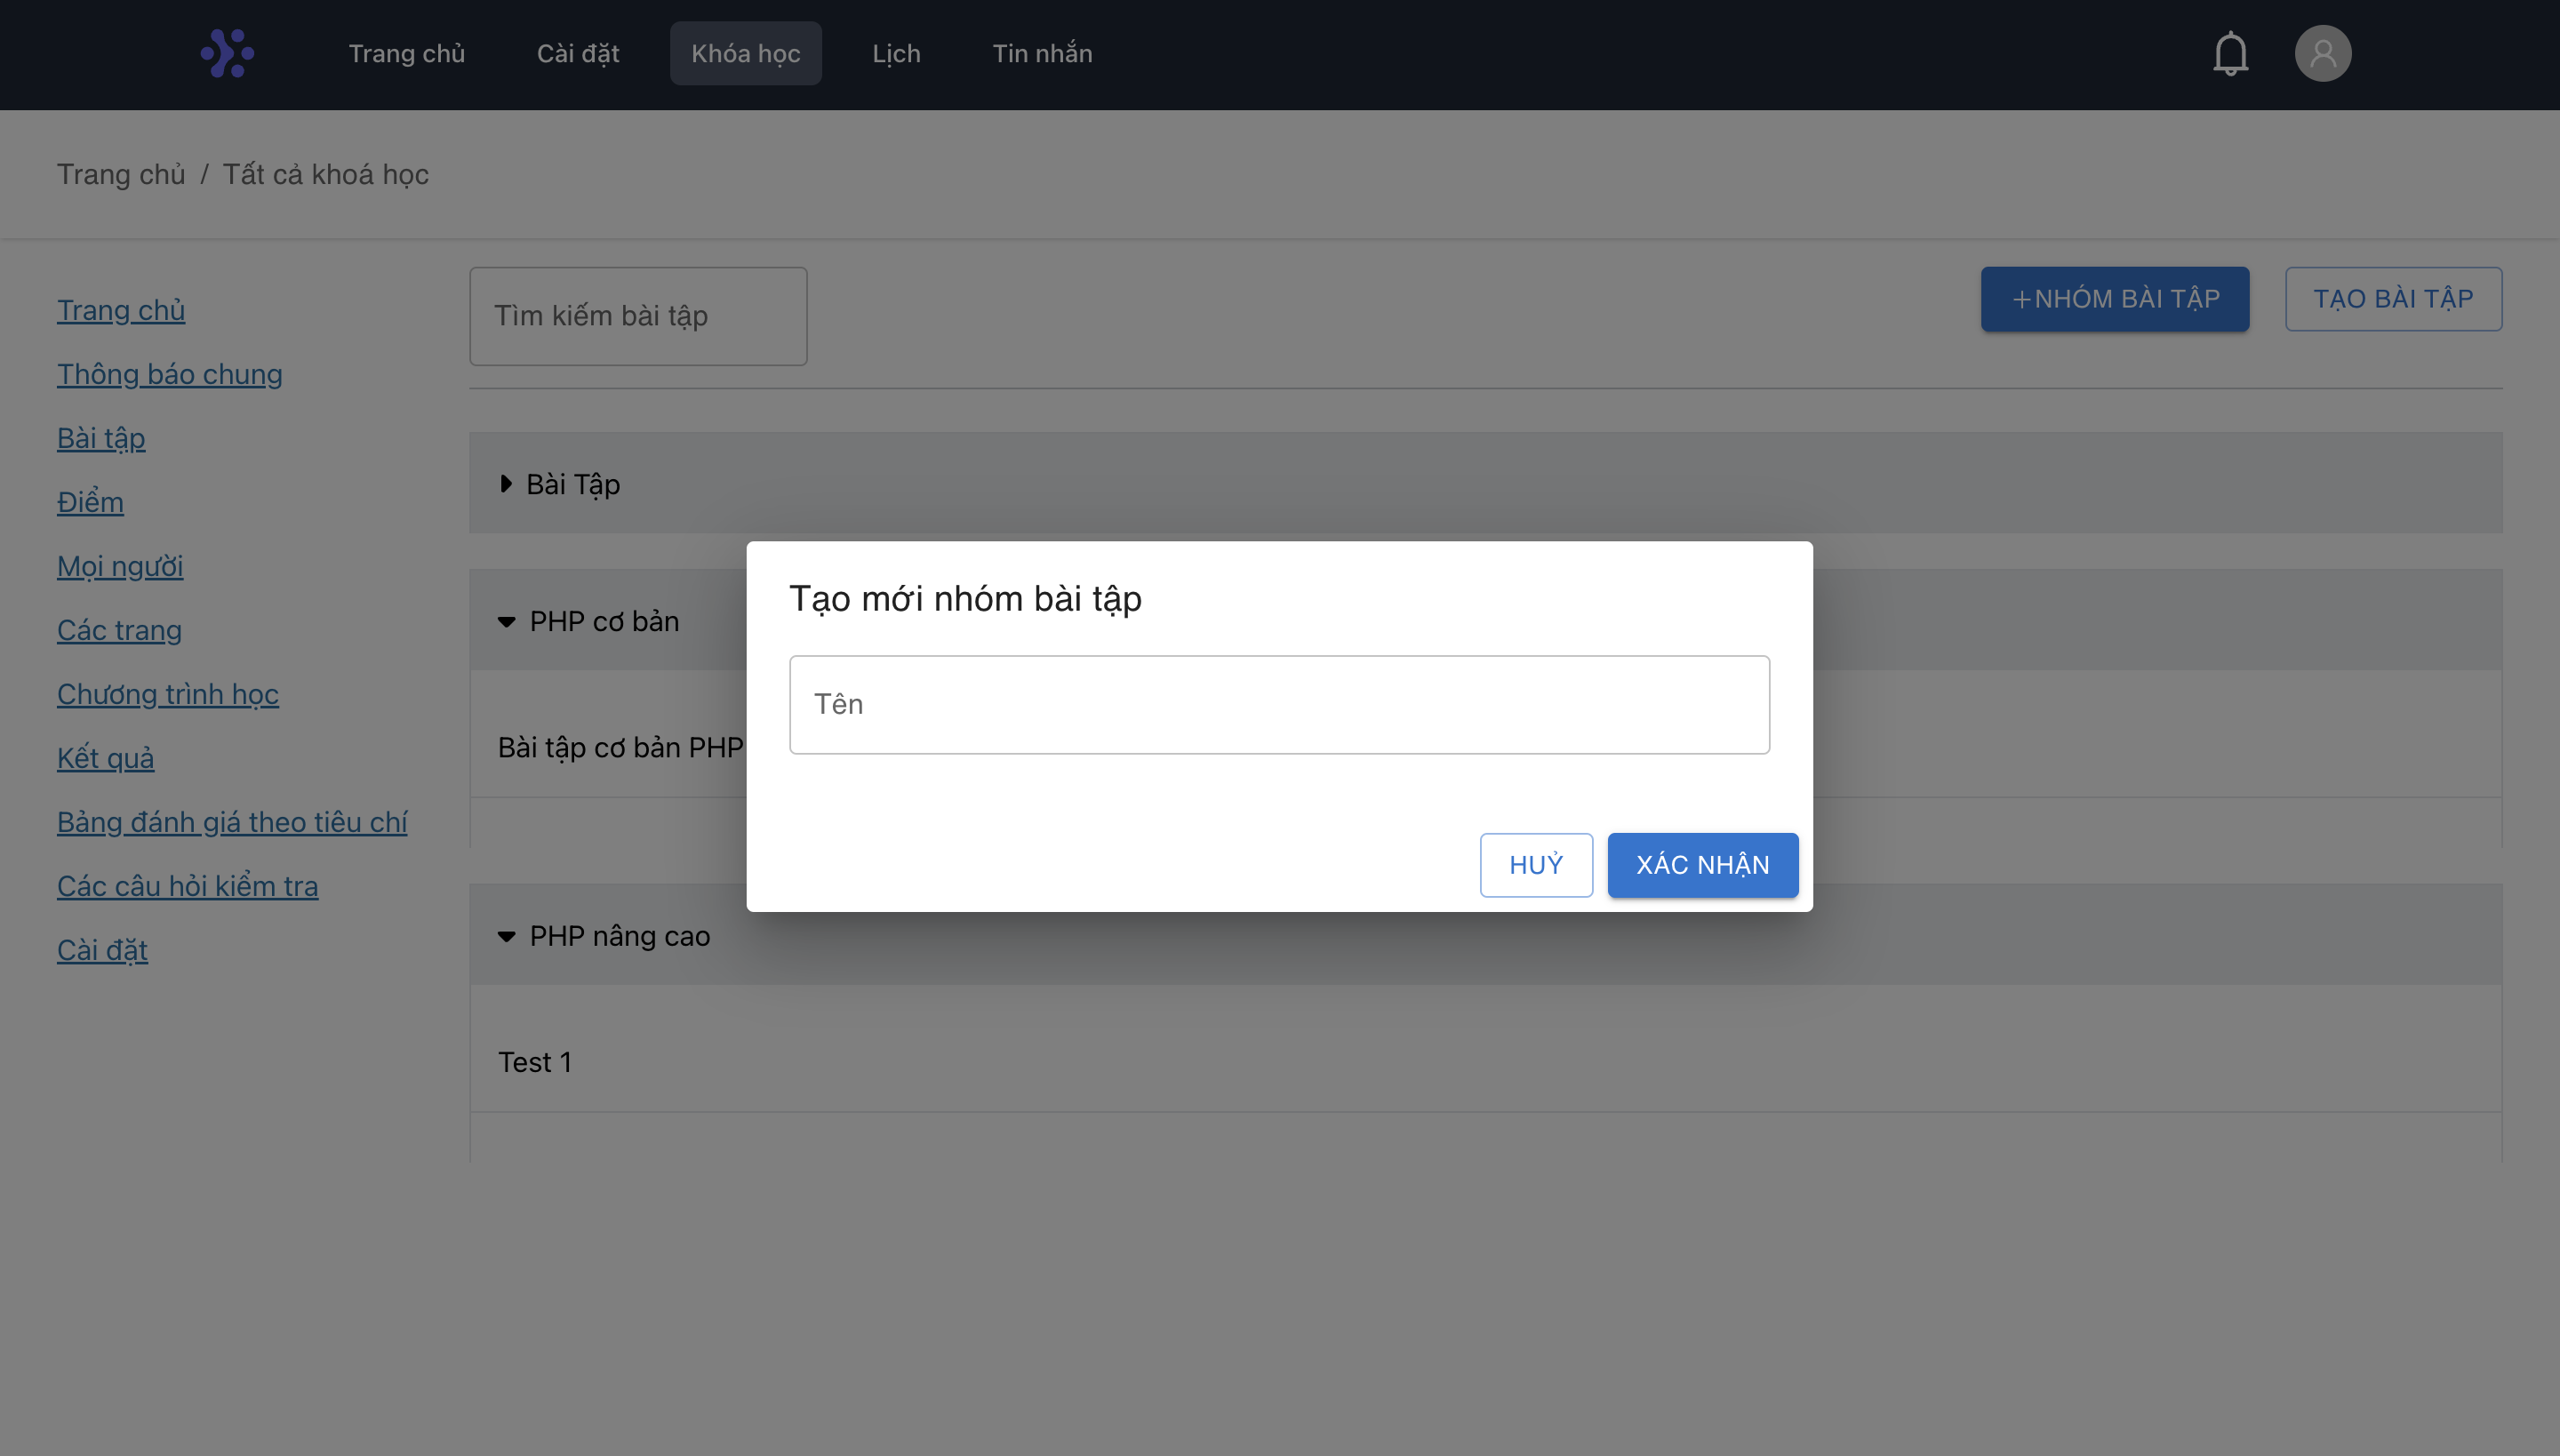
\includegraphics[scale=0.15]{8-tao-moi-nhom-bai-tap}
        \caption{Màn hình Tạo nhóm}
        \label{fig:tao-moi-nhom-bai-tap}
    \end{figure}

    \begin{figure}[ht!]
        \centering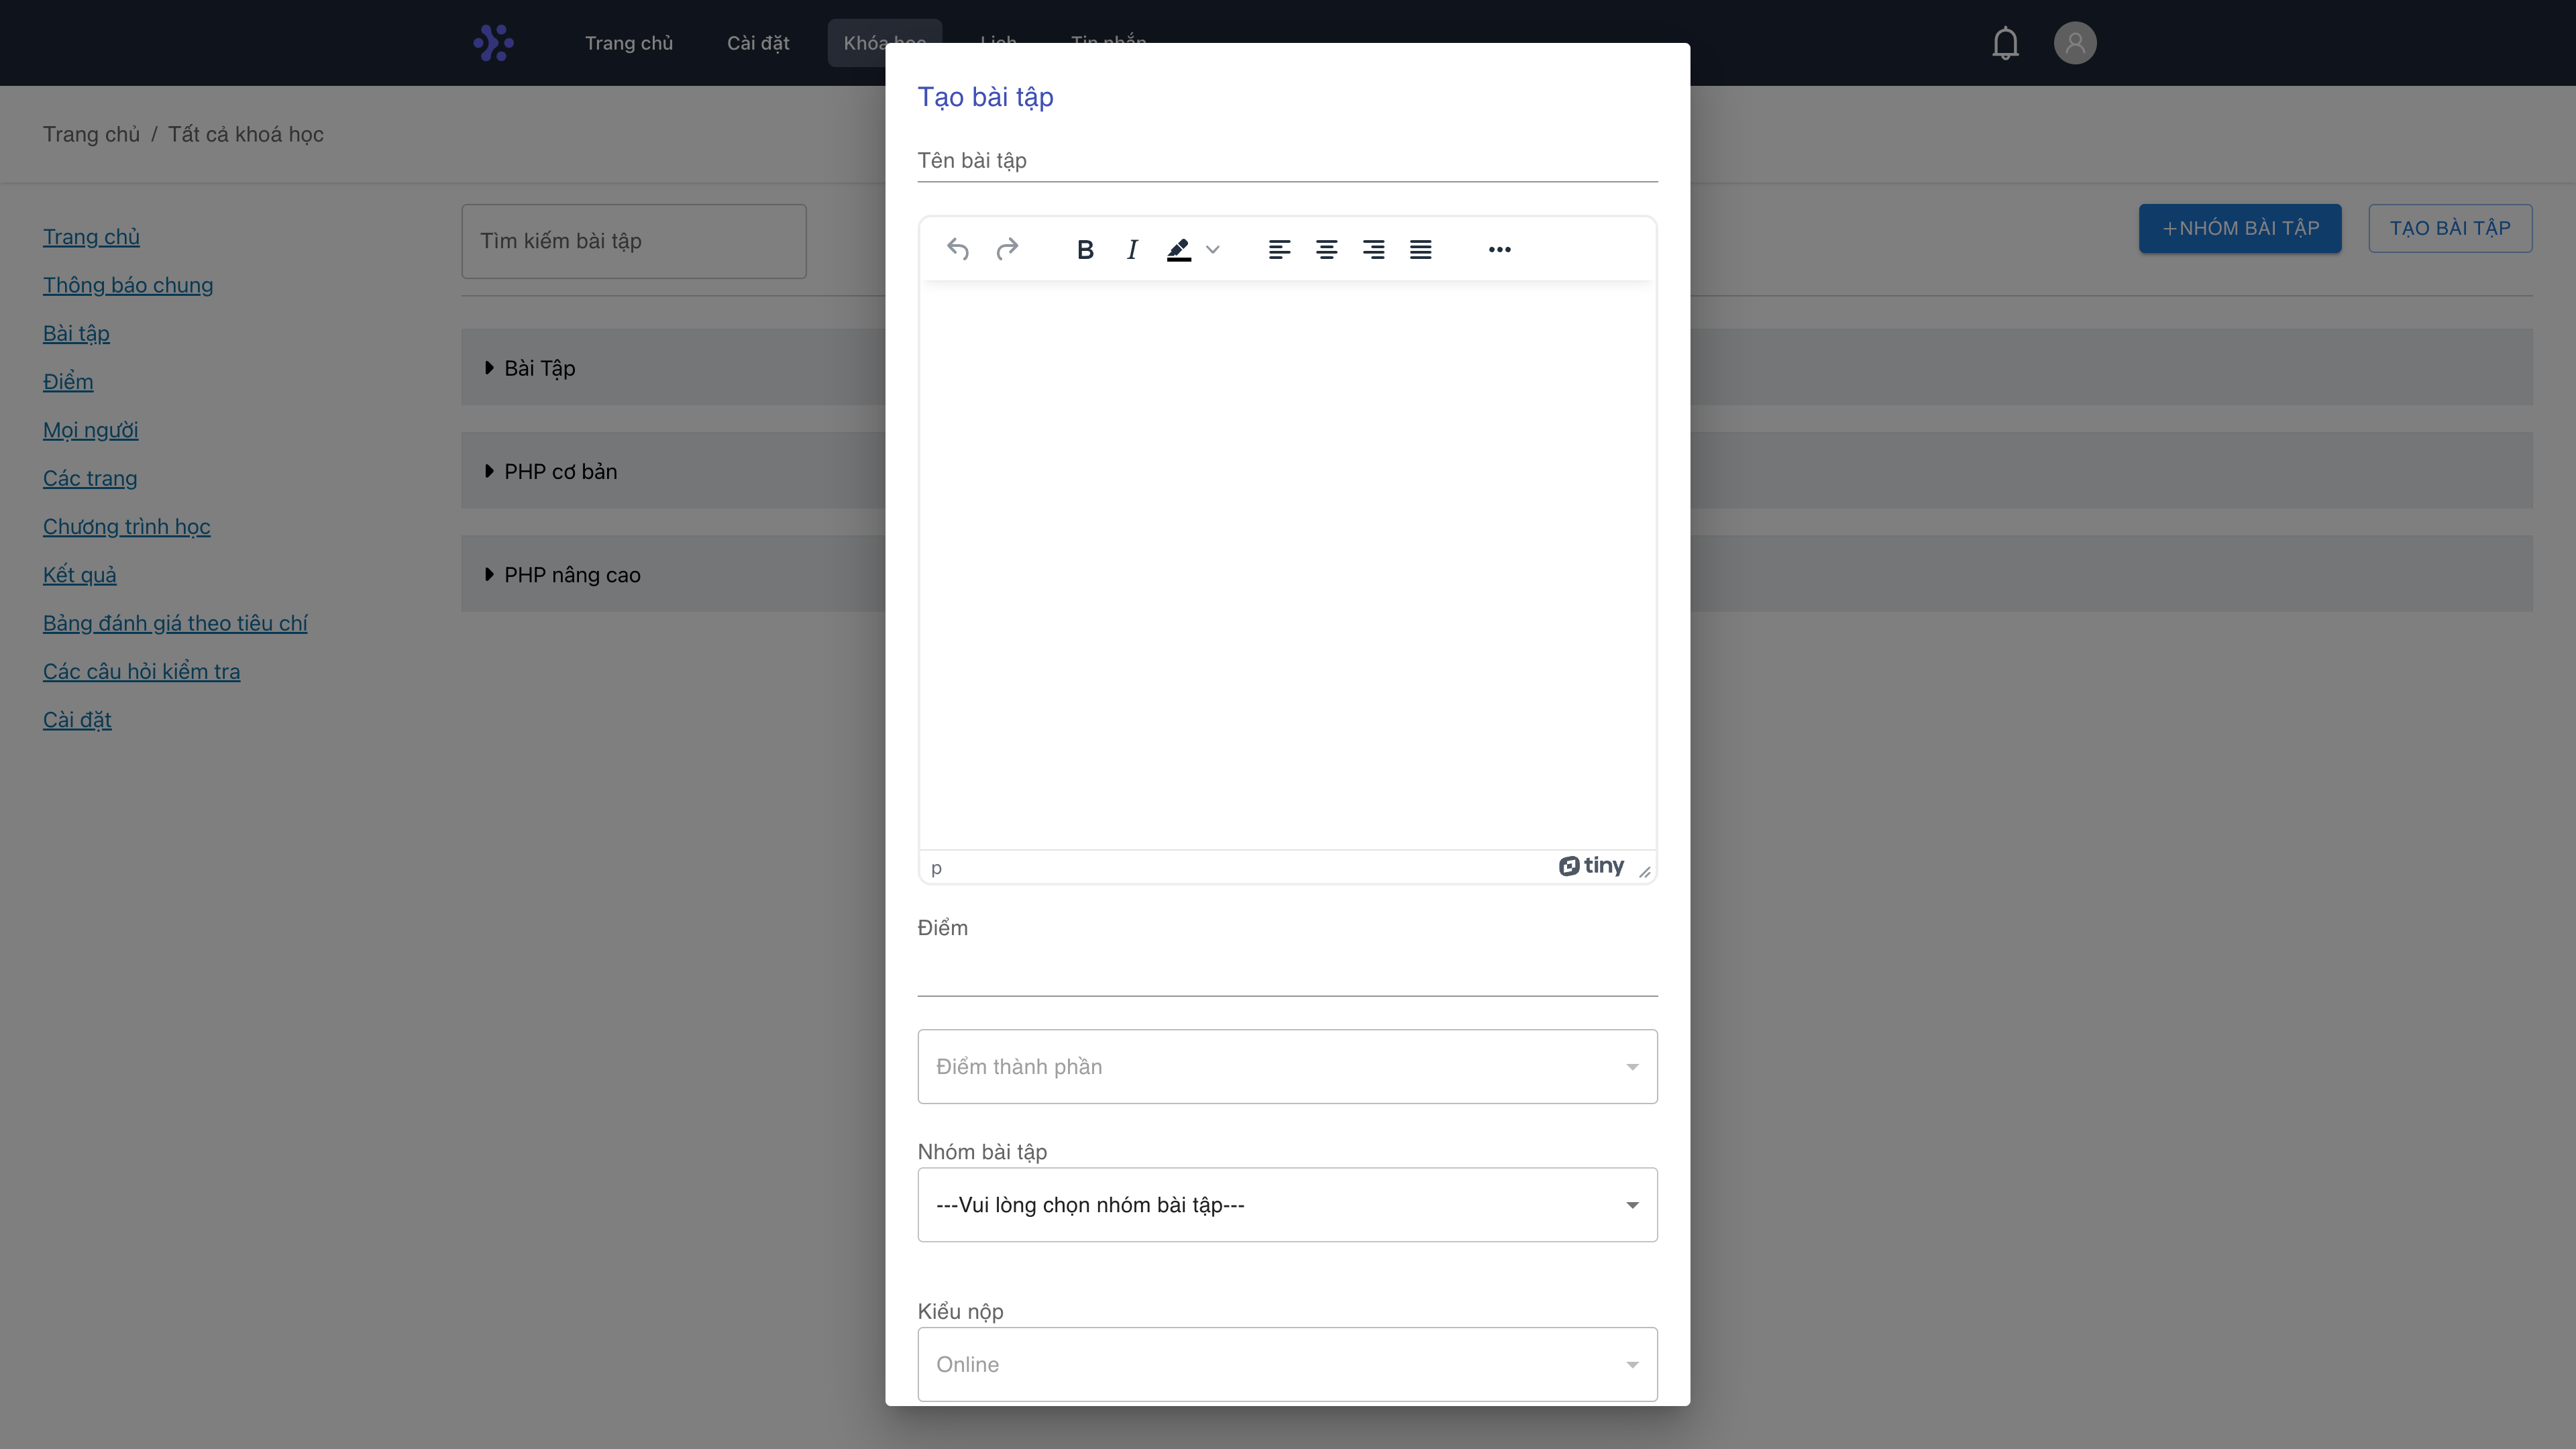
\includegraphics[scale=0.15]{9-tao-bai-tap}
        \caption{Màn hình Tạo bài tập}
        \label{fig:tao-moi-bai-tap}
    \end{figure}

    \begin{figure}[ht!]
        \centering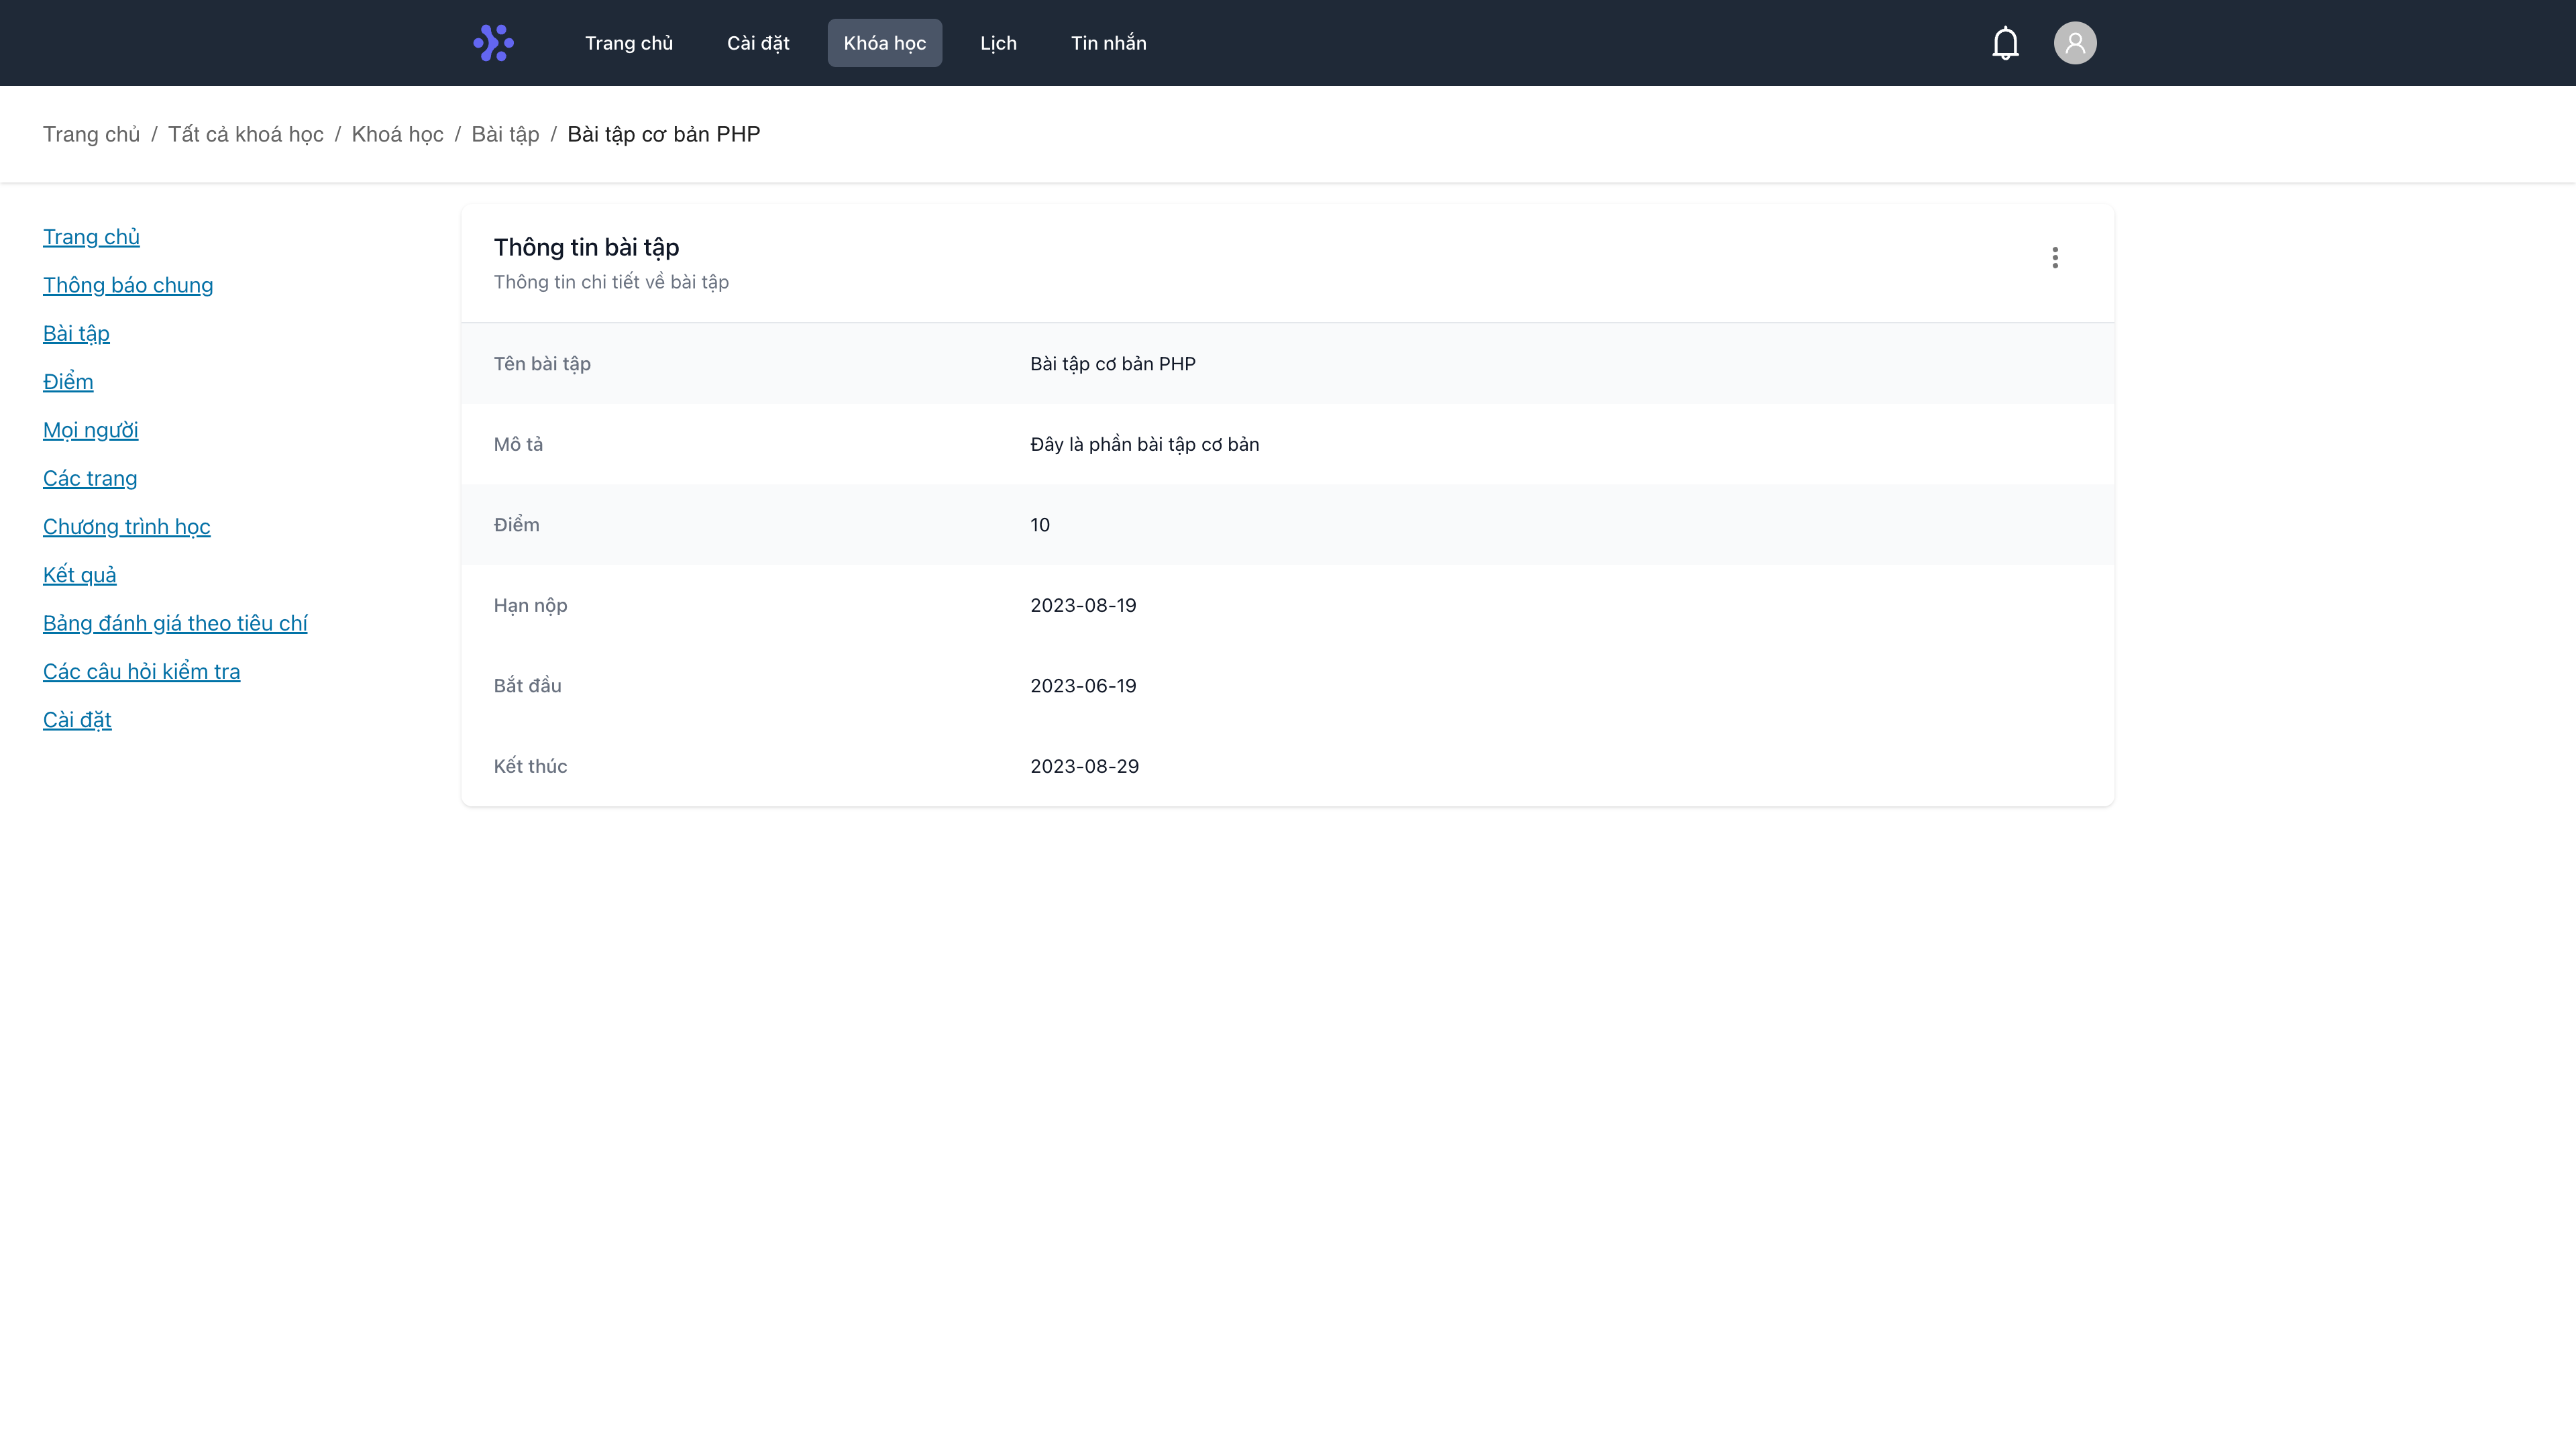
\includegraphics[scale=0.15]{10-chi-tiet-bai-tap}
        \caption{Màn hình Chi tiết bài tập}
        \label{fig:chi-tiet-bai-tap}
    \end{figure}

    \begin{figure}[ht!]
        \centering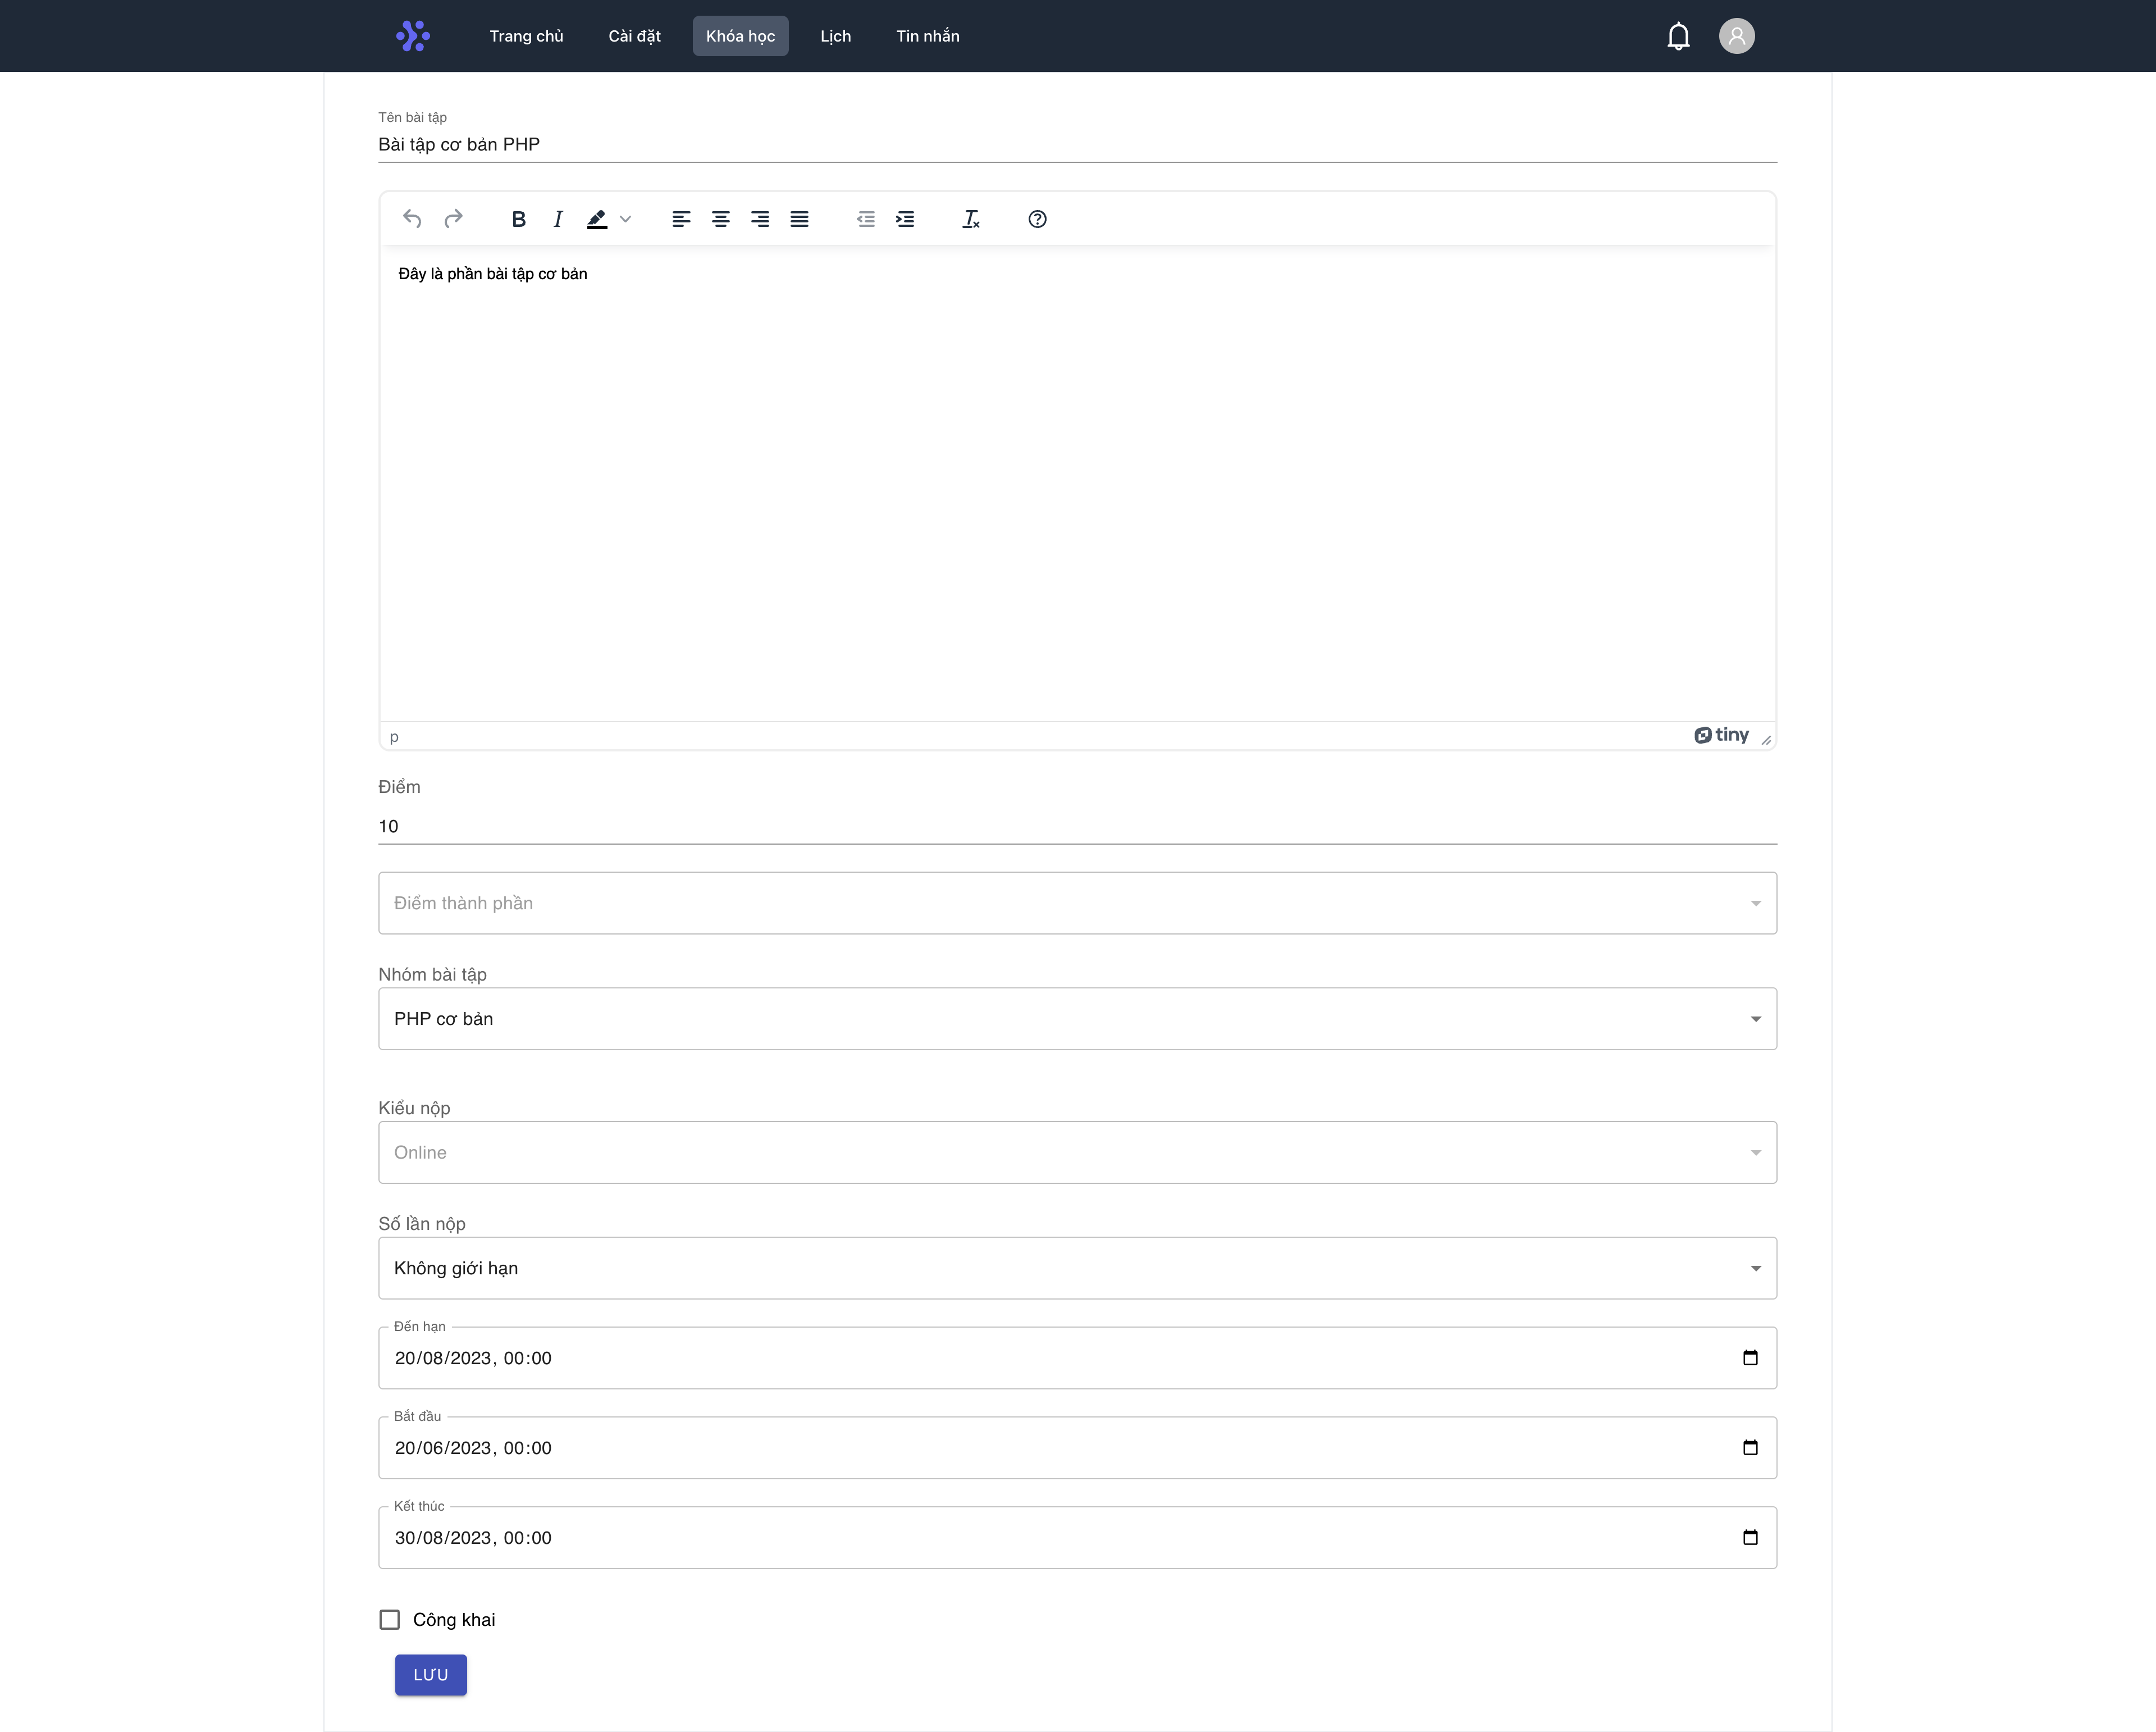
\includegraphics[scale=0.15]{11-chinh-sua-bai-tap}
        \caption{Màn hình Chỉnh sửa bài tập}
        \label{fig:chinh-sua-bai-tap}
    \end{figure}

    \begin{figure}[ht!]
        \centering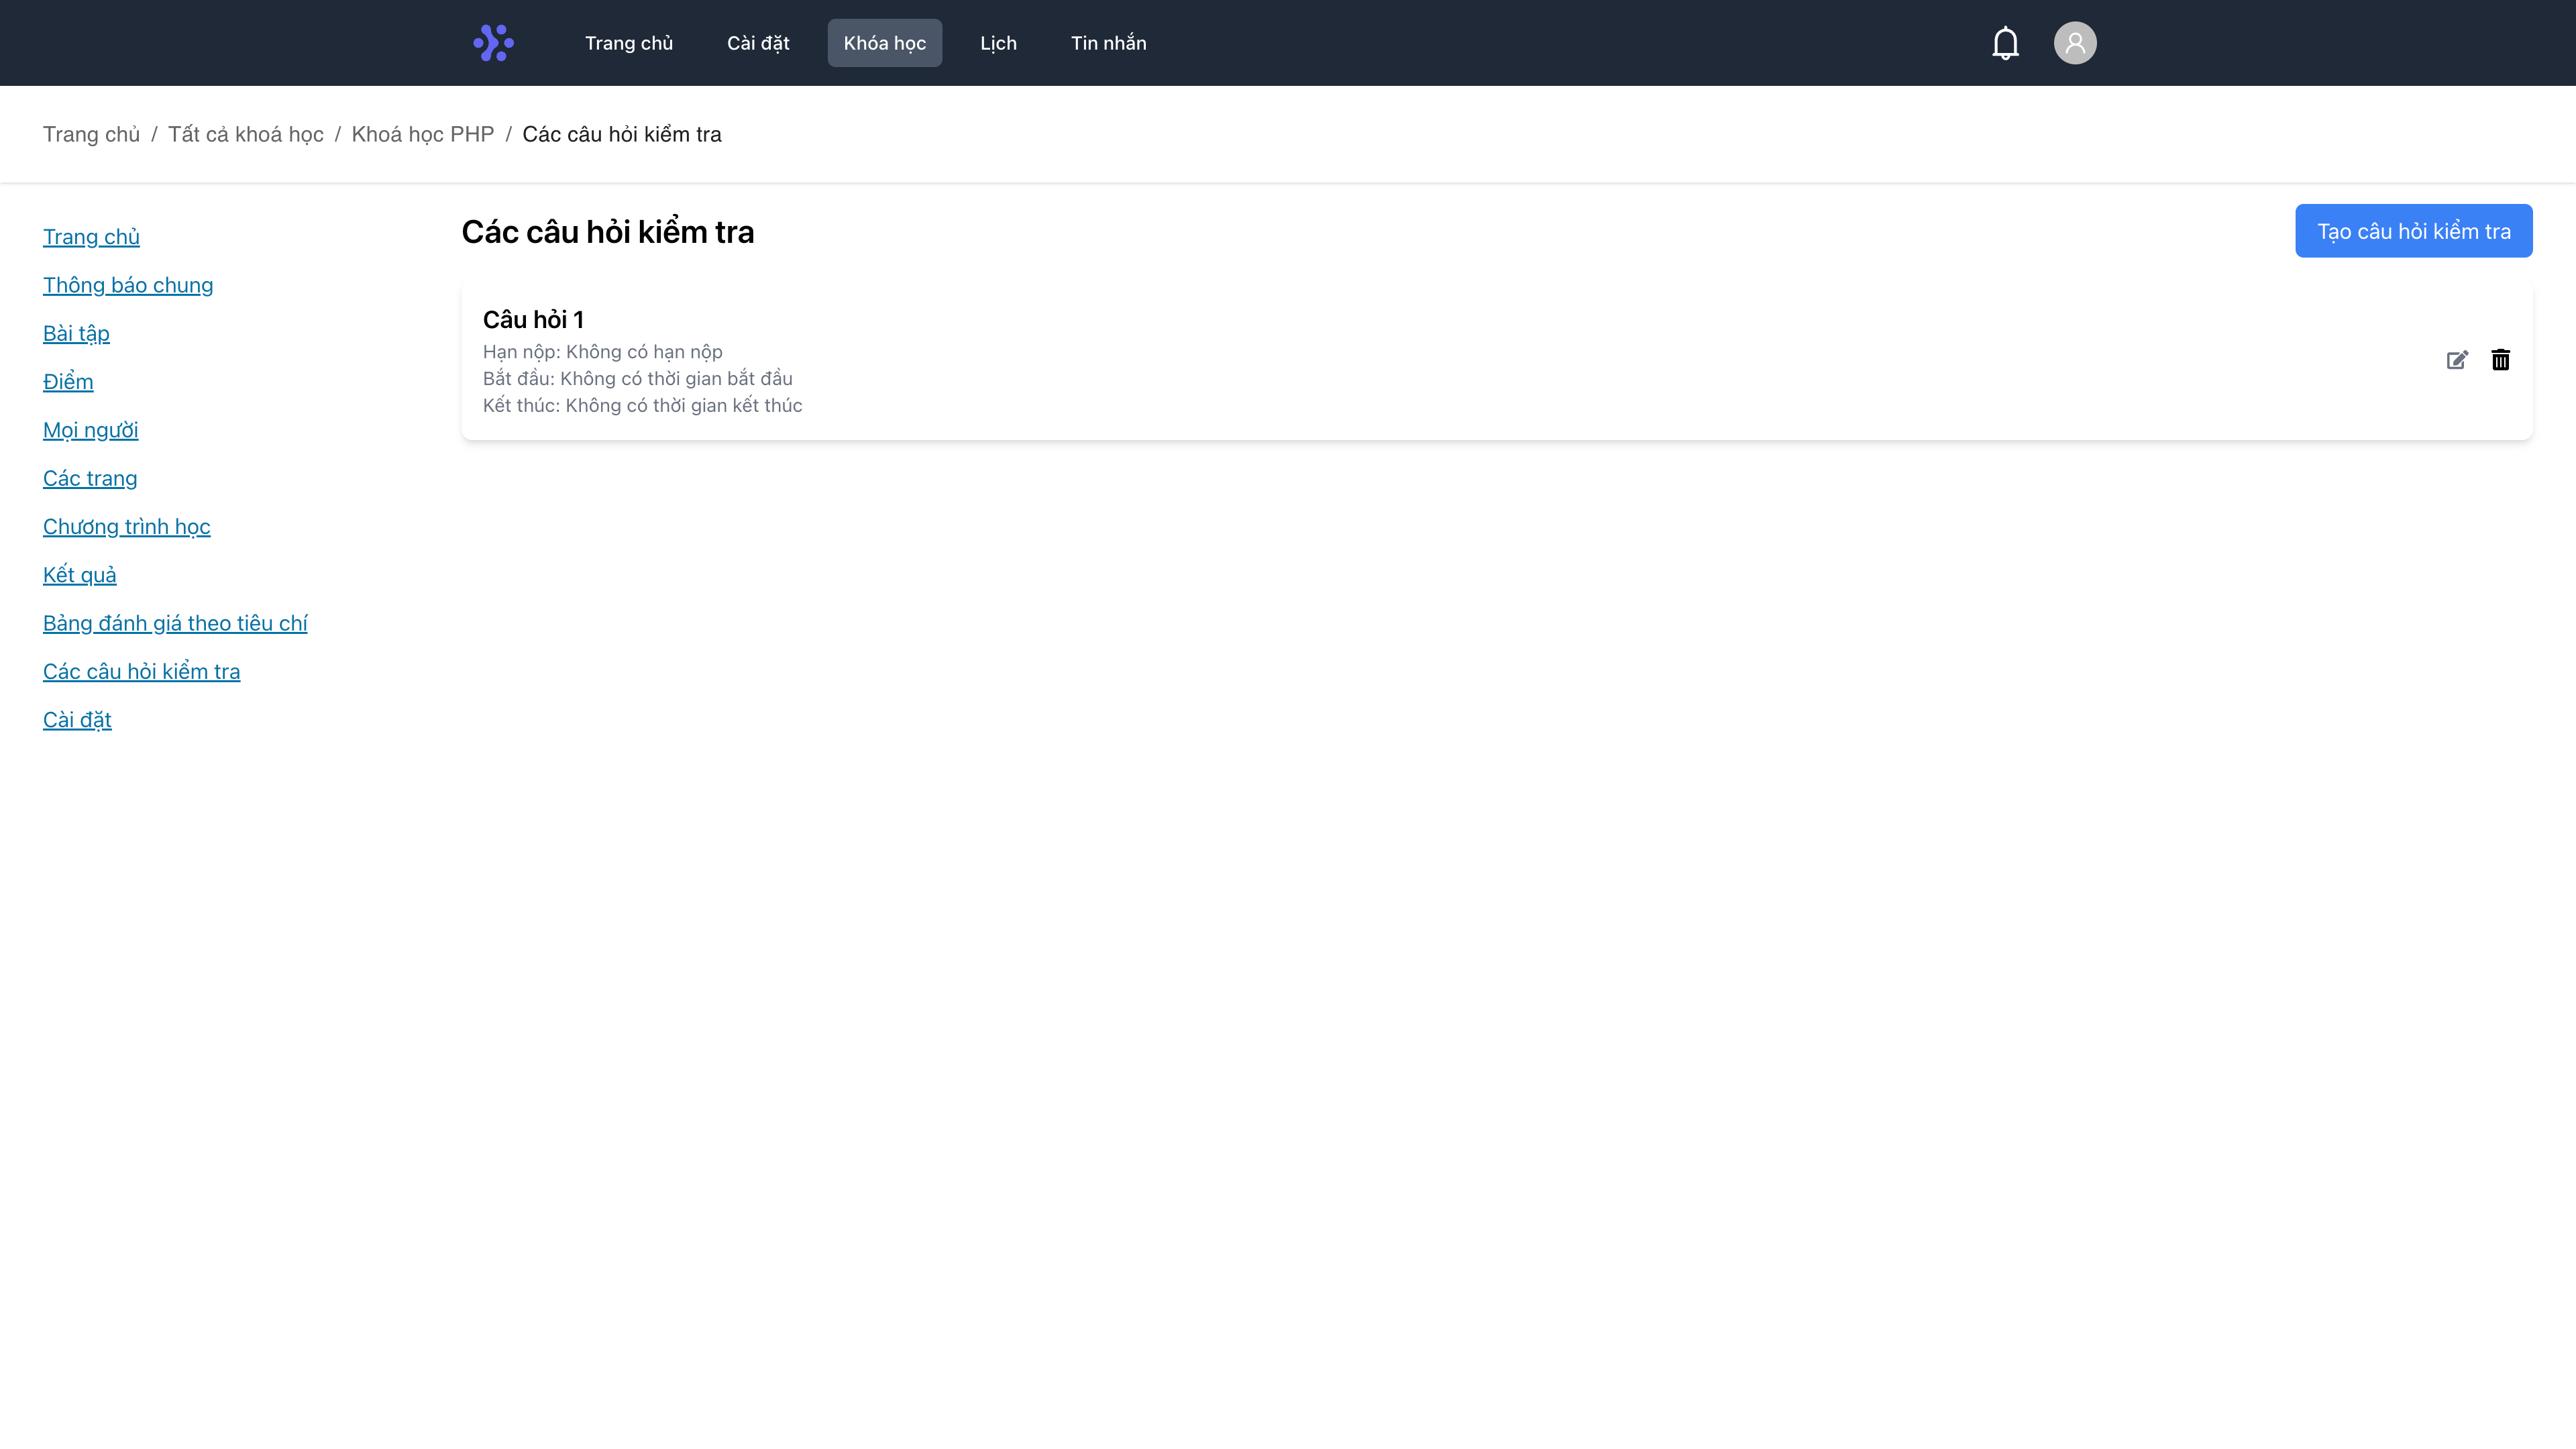
\includegraphics[scale=0.15]{cau-hoi-kiem-tra}
        \caption{Câu hỏi kiểm tra}
        \label{fig:cau-hoi-kiem-tra}
    \end{figure}

     \begin{figure}[ht!]
        \centering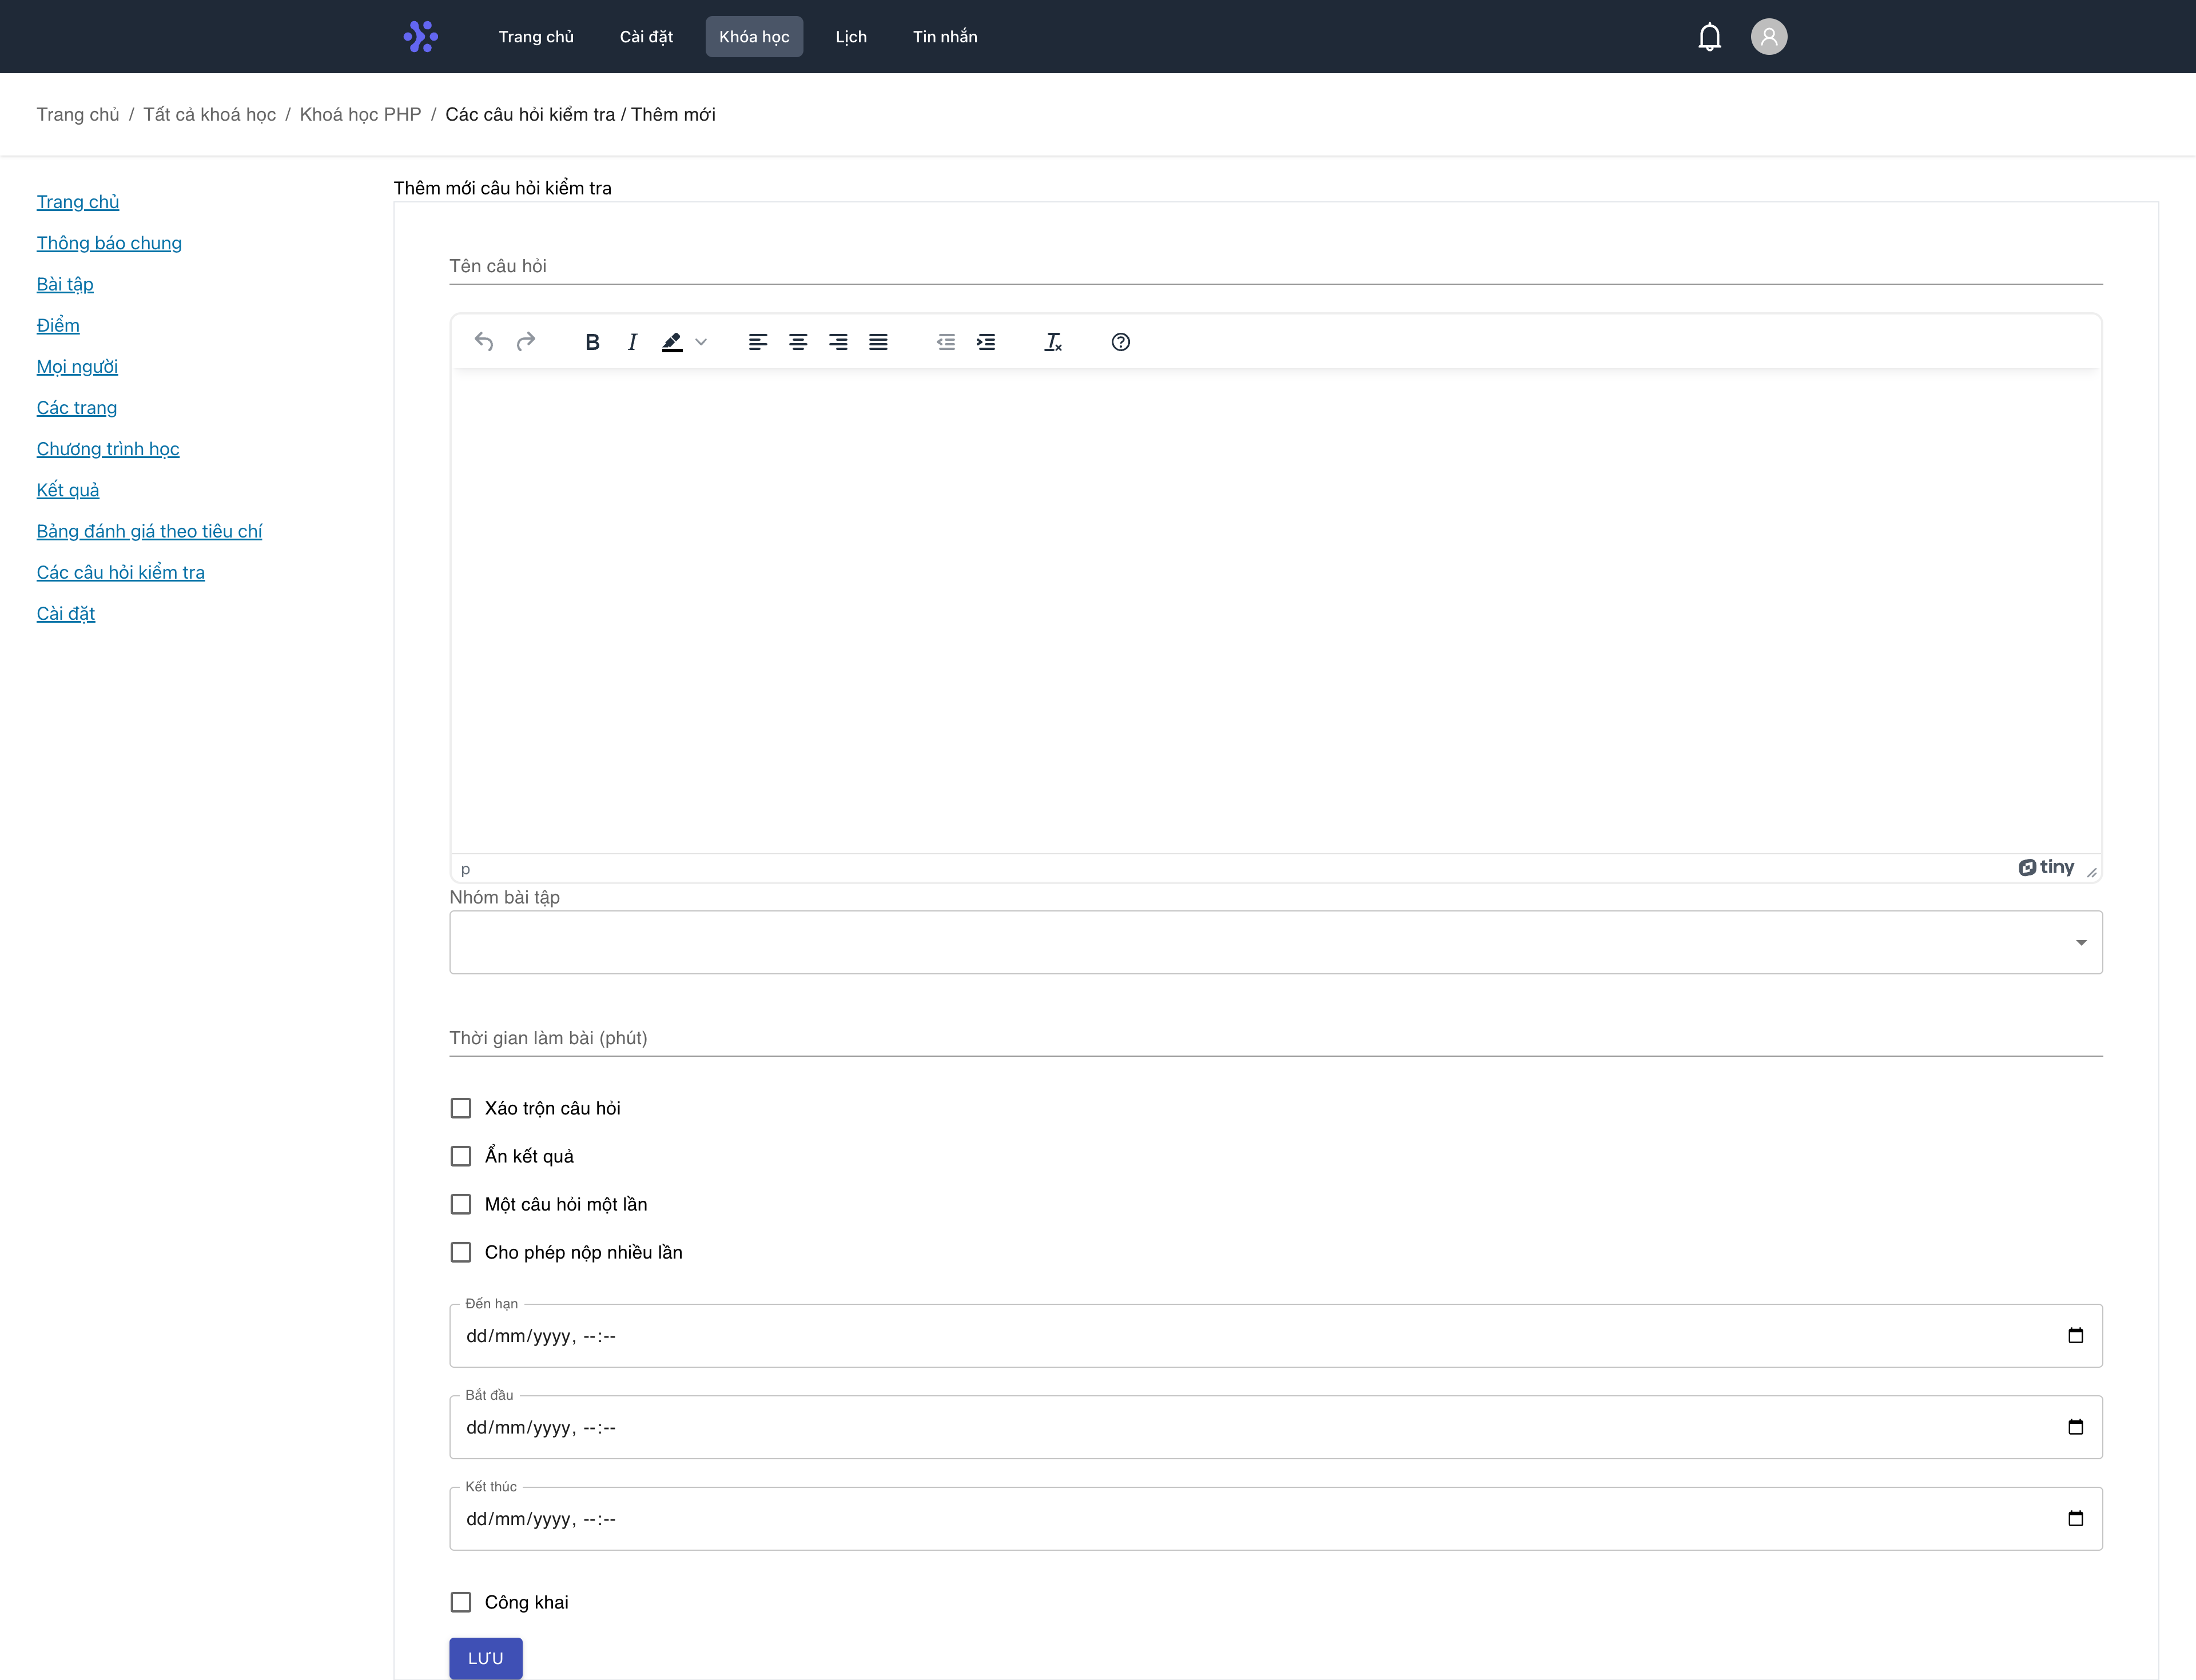
\includegraphics[scale=0.15]{them-moi-cau-hoi-kiem-tra}
        \caption{Thêm câu hỏi kiểm tra}
        \label{fig:them-moi-cau-hoi-kiem-tra}
    \end{figure}

     \begin{figure}[ht!]
        \centering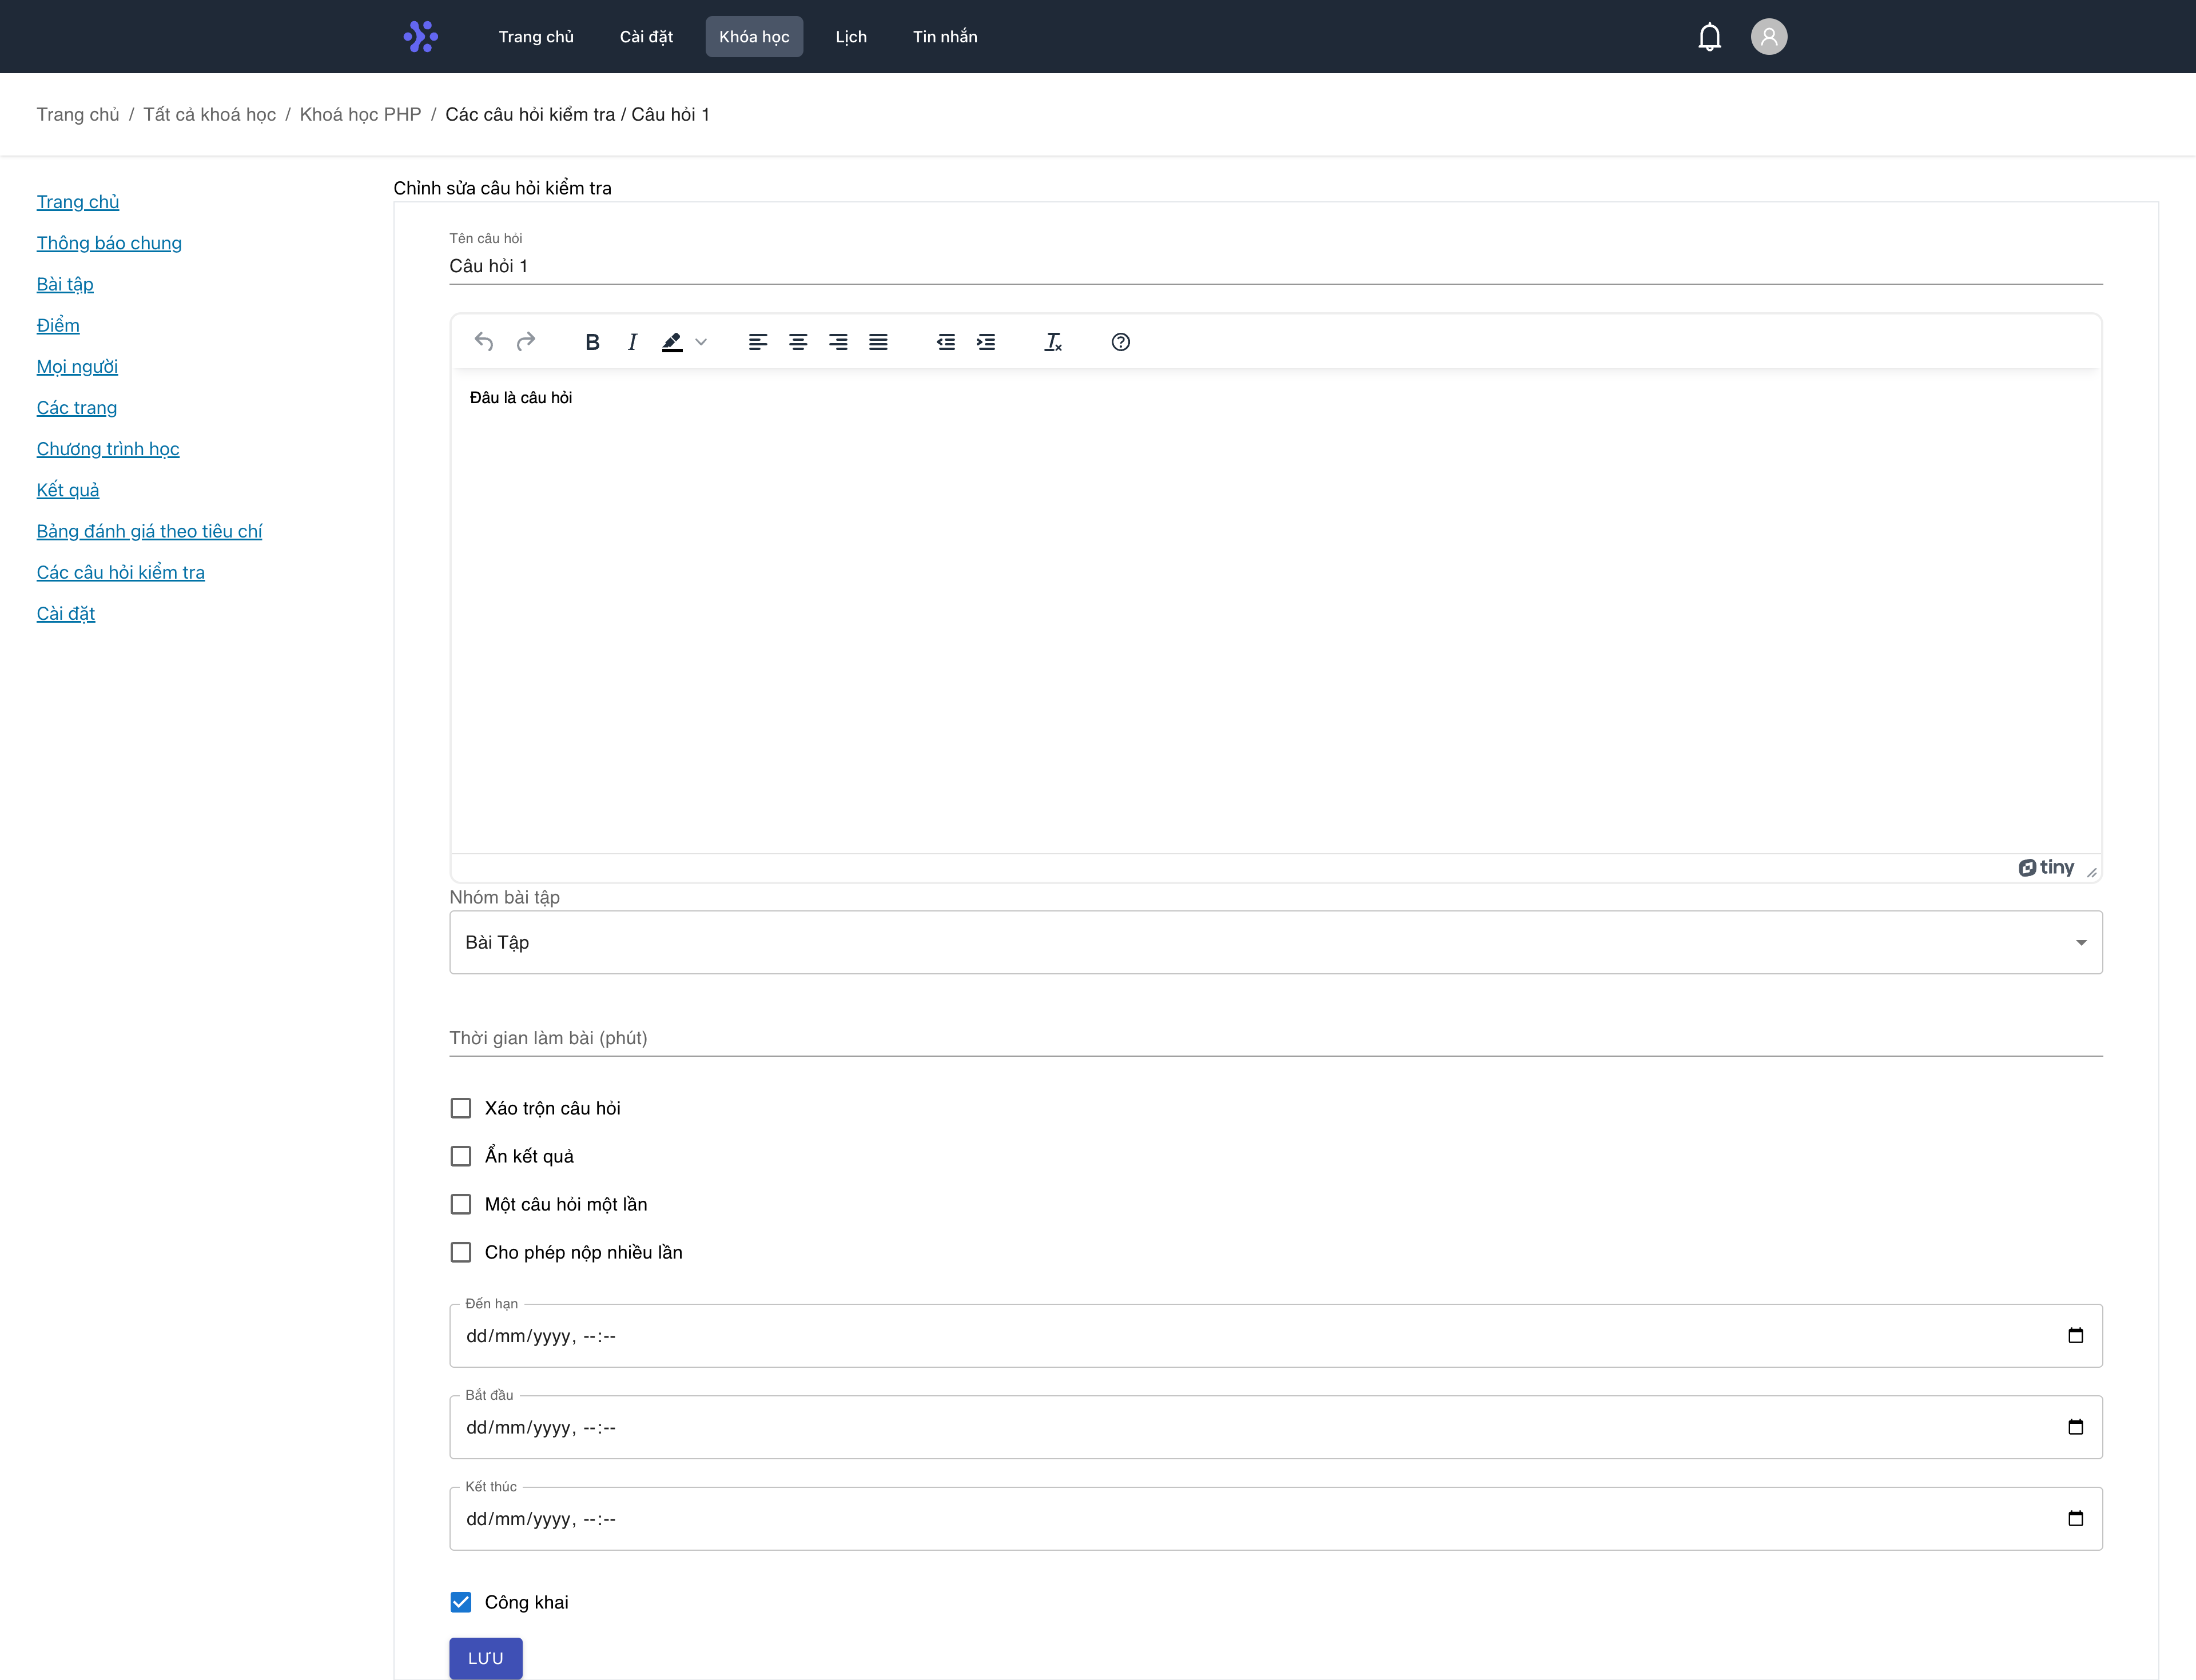
\includegraphics[scale=0.15]{chinh-sua-cau-hoi-kiem-tra}
        \caption{Chỉnh sửa câu hỏi kiểm tra}
        \label{fig:chinh-sua-cau-hoi-kiem-tra}
    \end{figure}

     \begin{figure}[ht!]
        \centering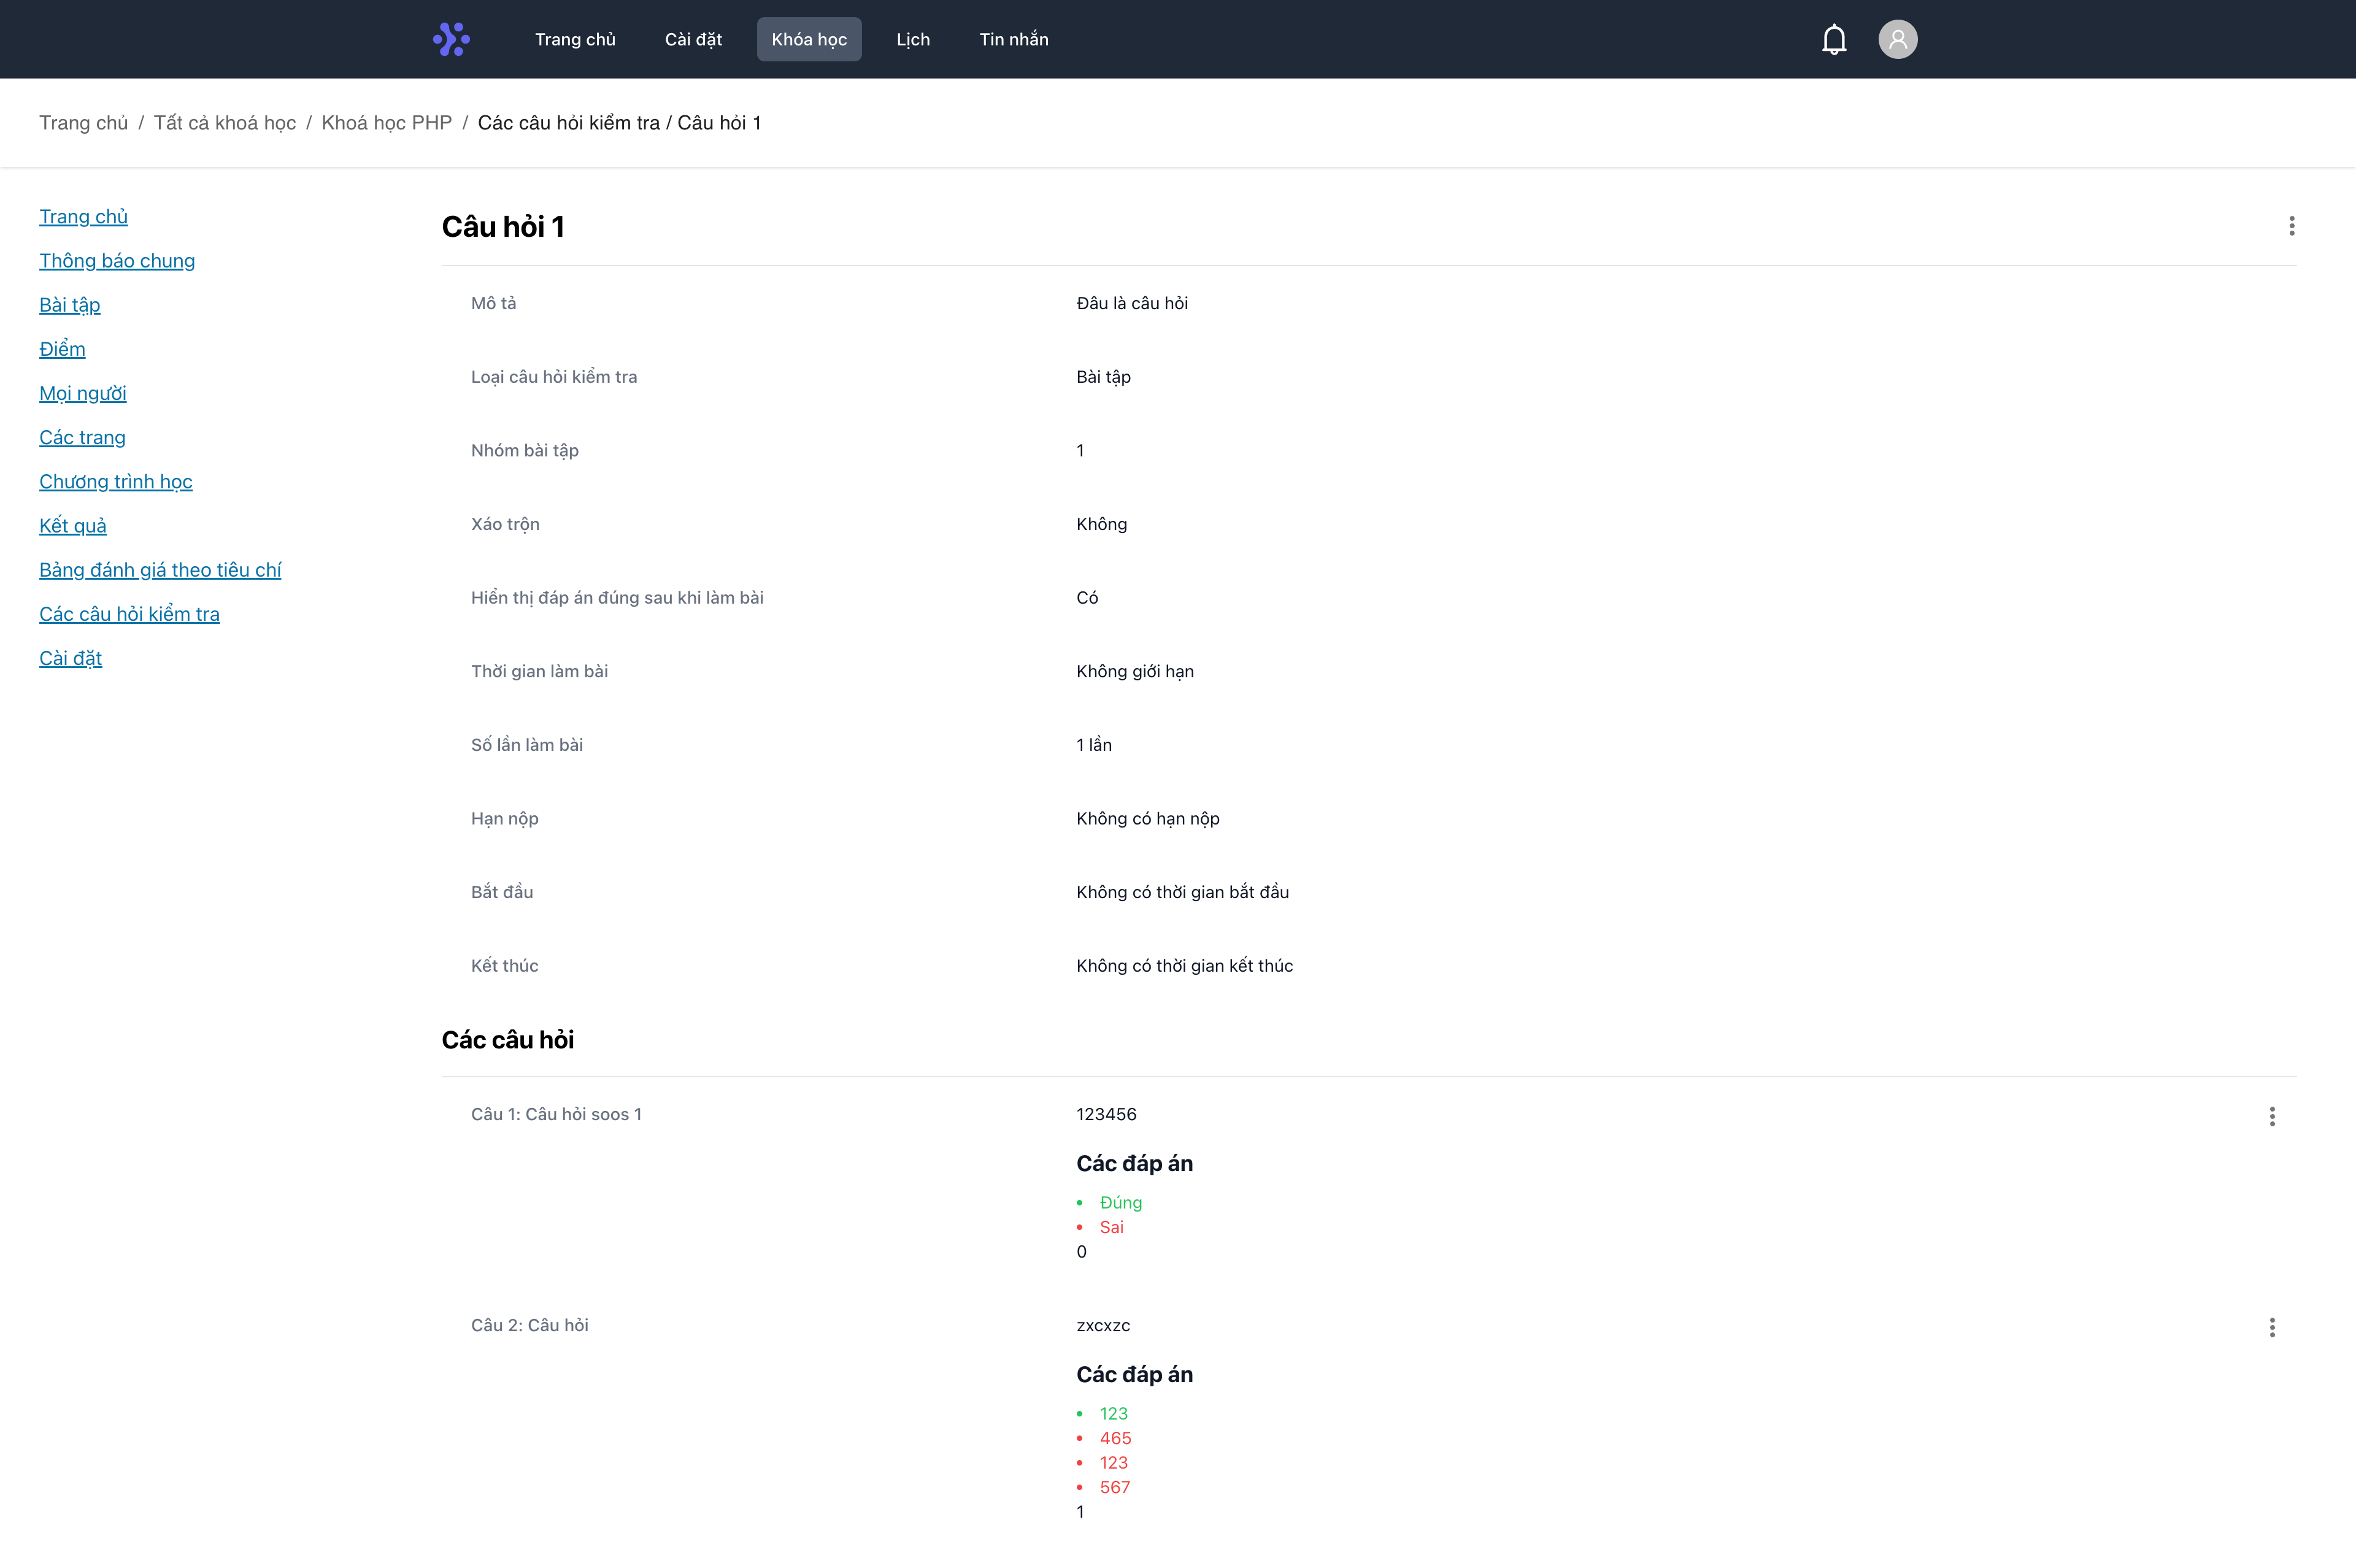
\includegraphics[scale=0.15]{chi-tiet-cau-hoi-kiem-tra}
        \caption{Chi tiết câu hỏi kiểm tra}
        \label{fig:chi-tiet-cau-hoi-kiem-tra}
    \end{figure}

     \begin{figure}[ht!]
        \centering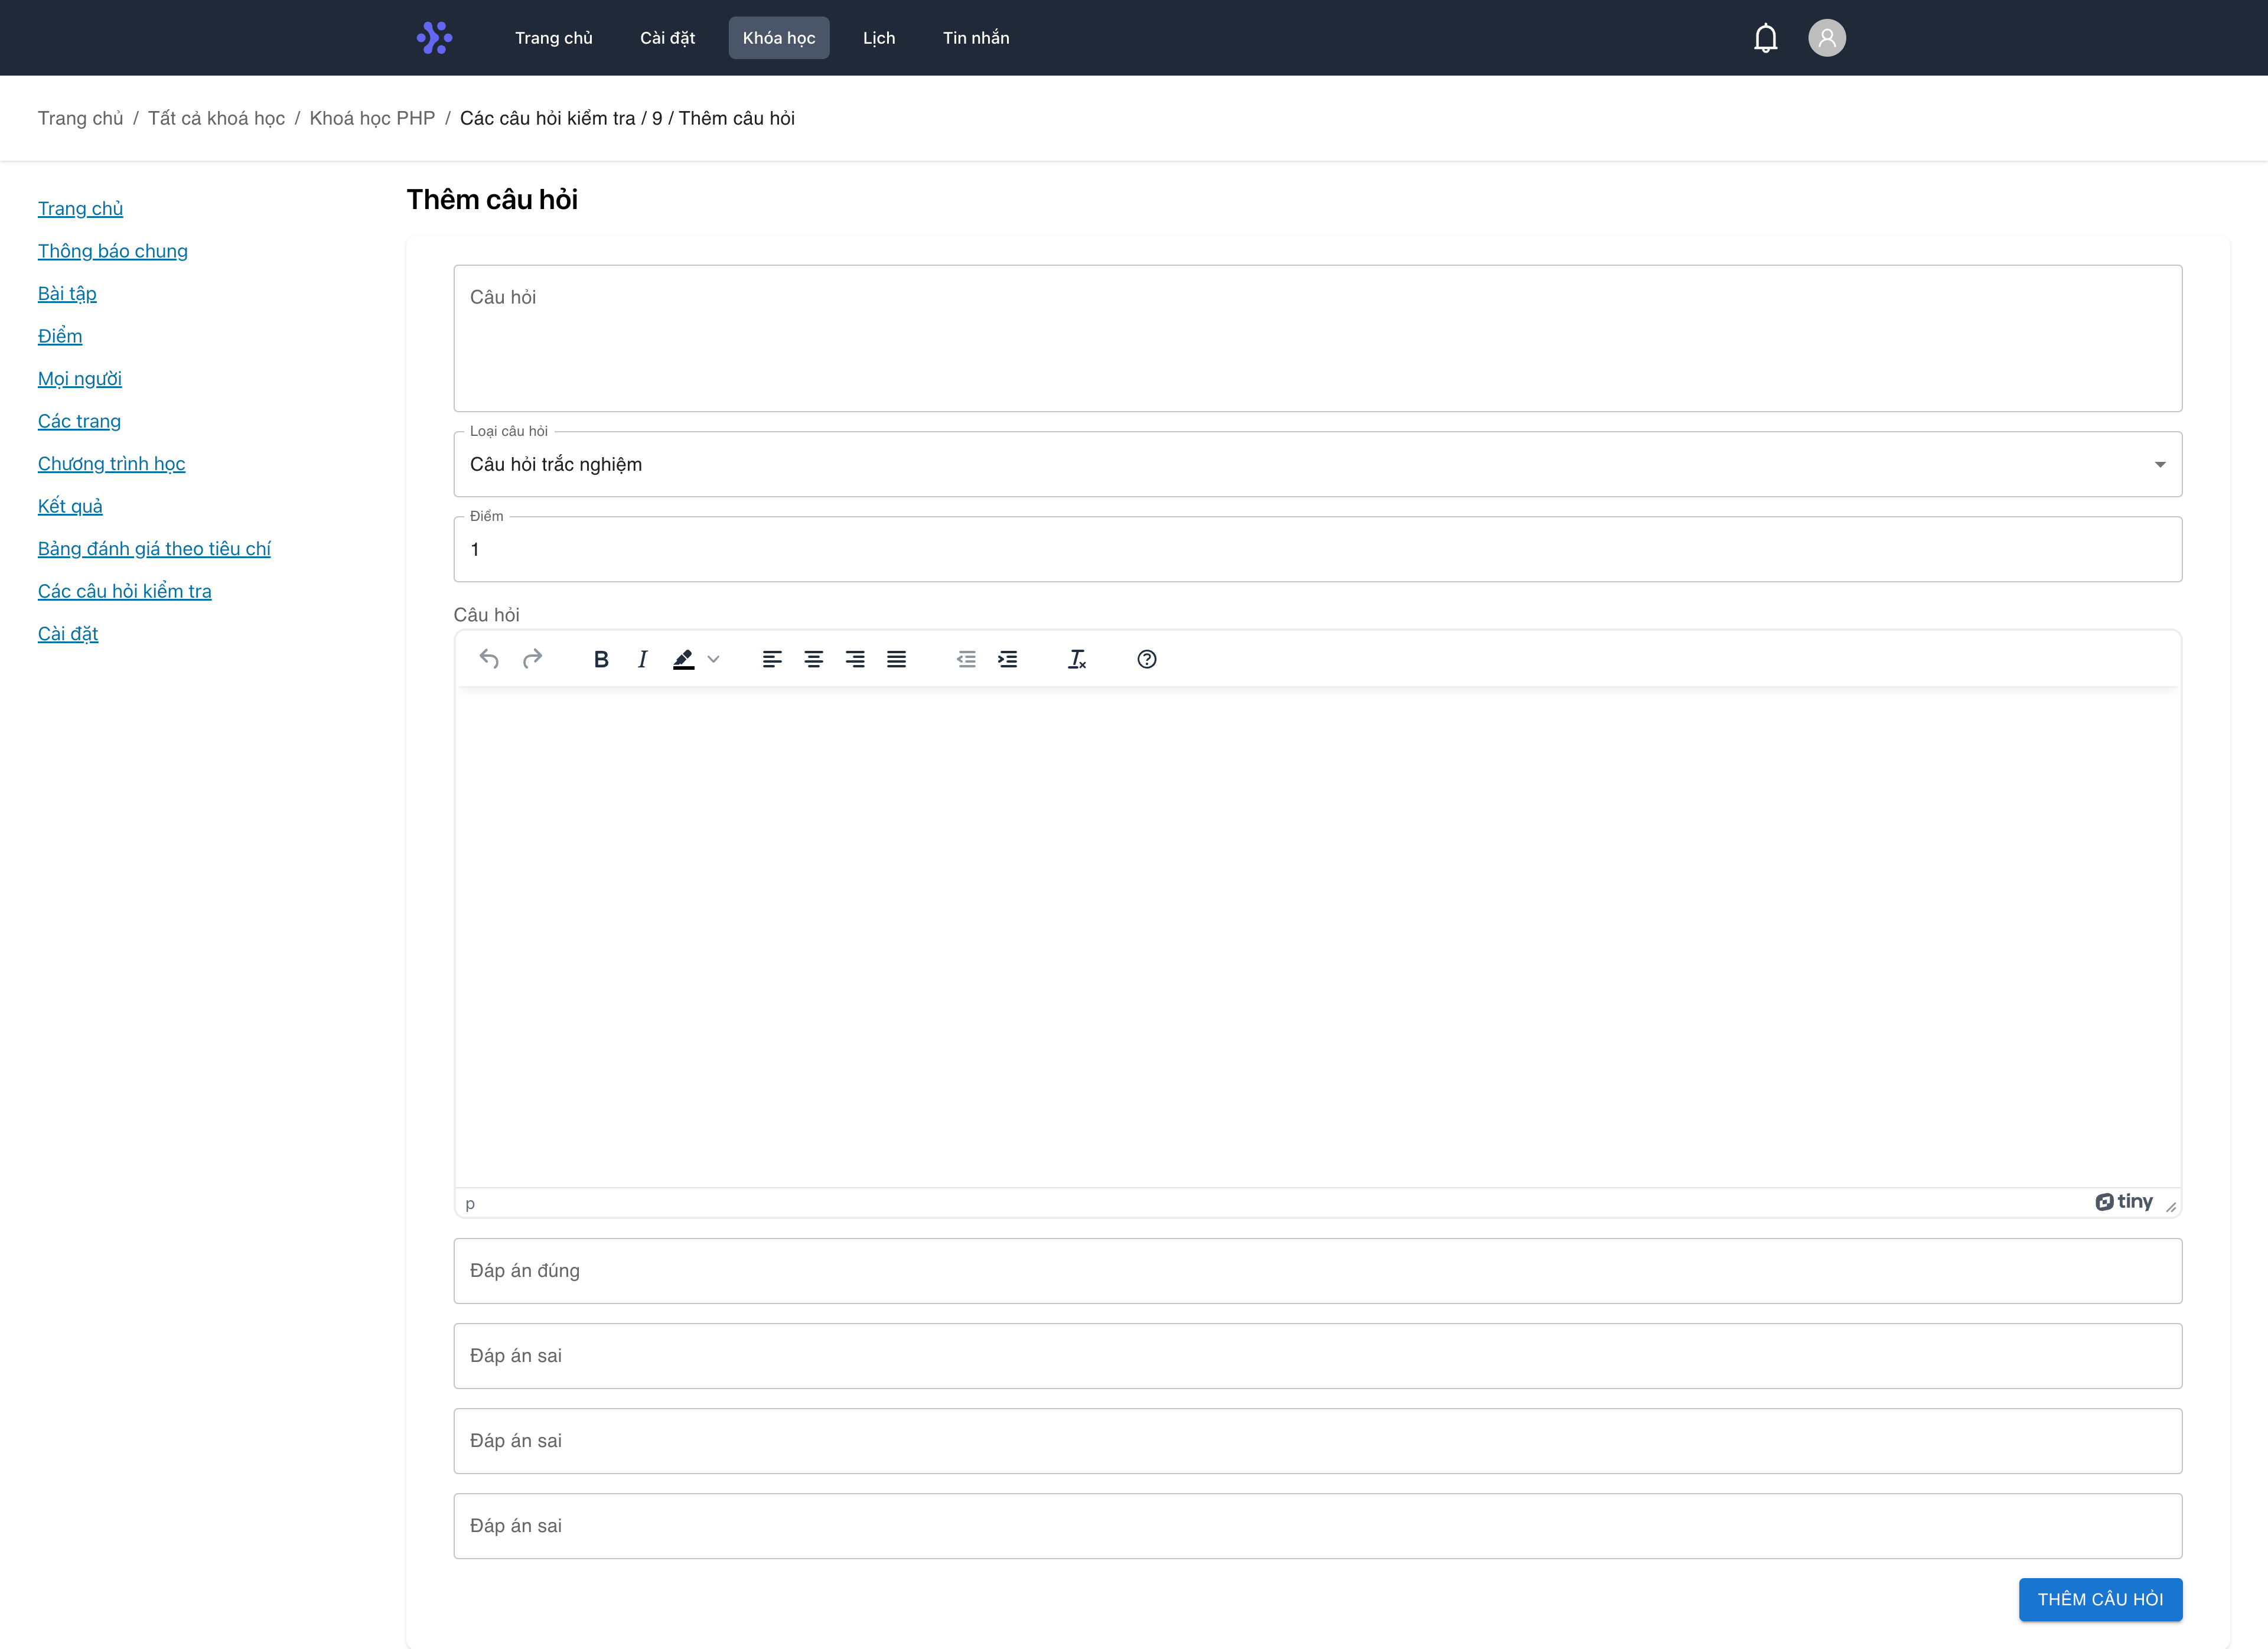
\includegraphics[scale=0.15]{them-cau-hoi}
        \caption{Thêm câu hỏi}
        \label{fig:them-cau-hoi}
    \end{figure}
    
     \begin{figure}[ht!]
        \centering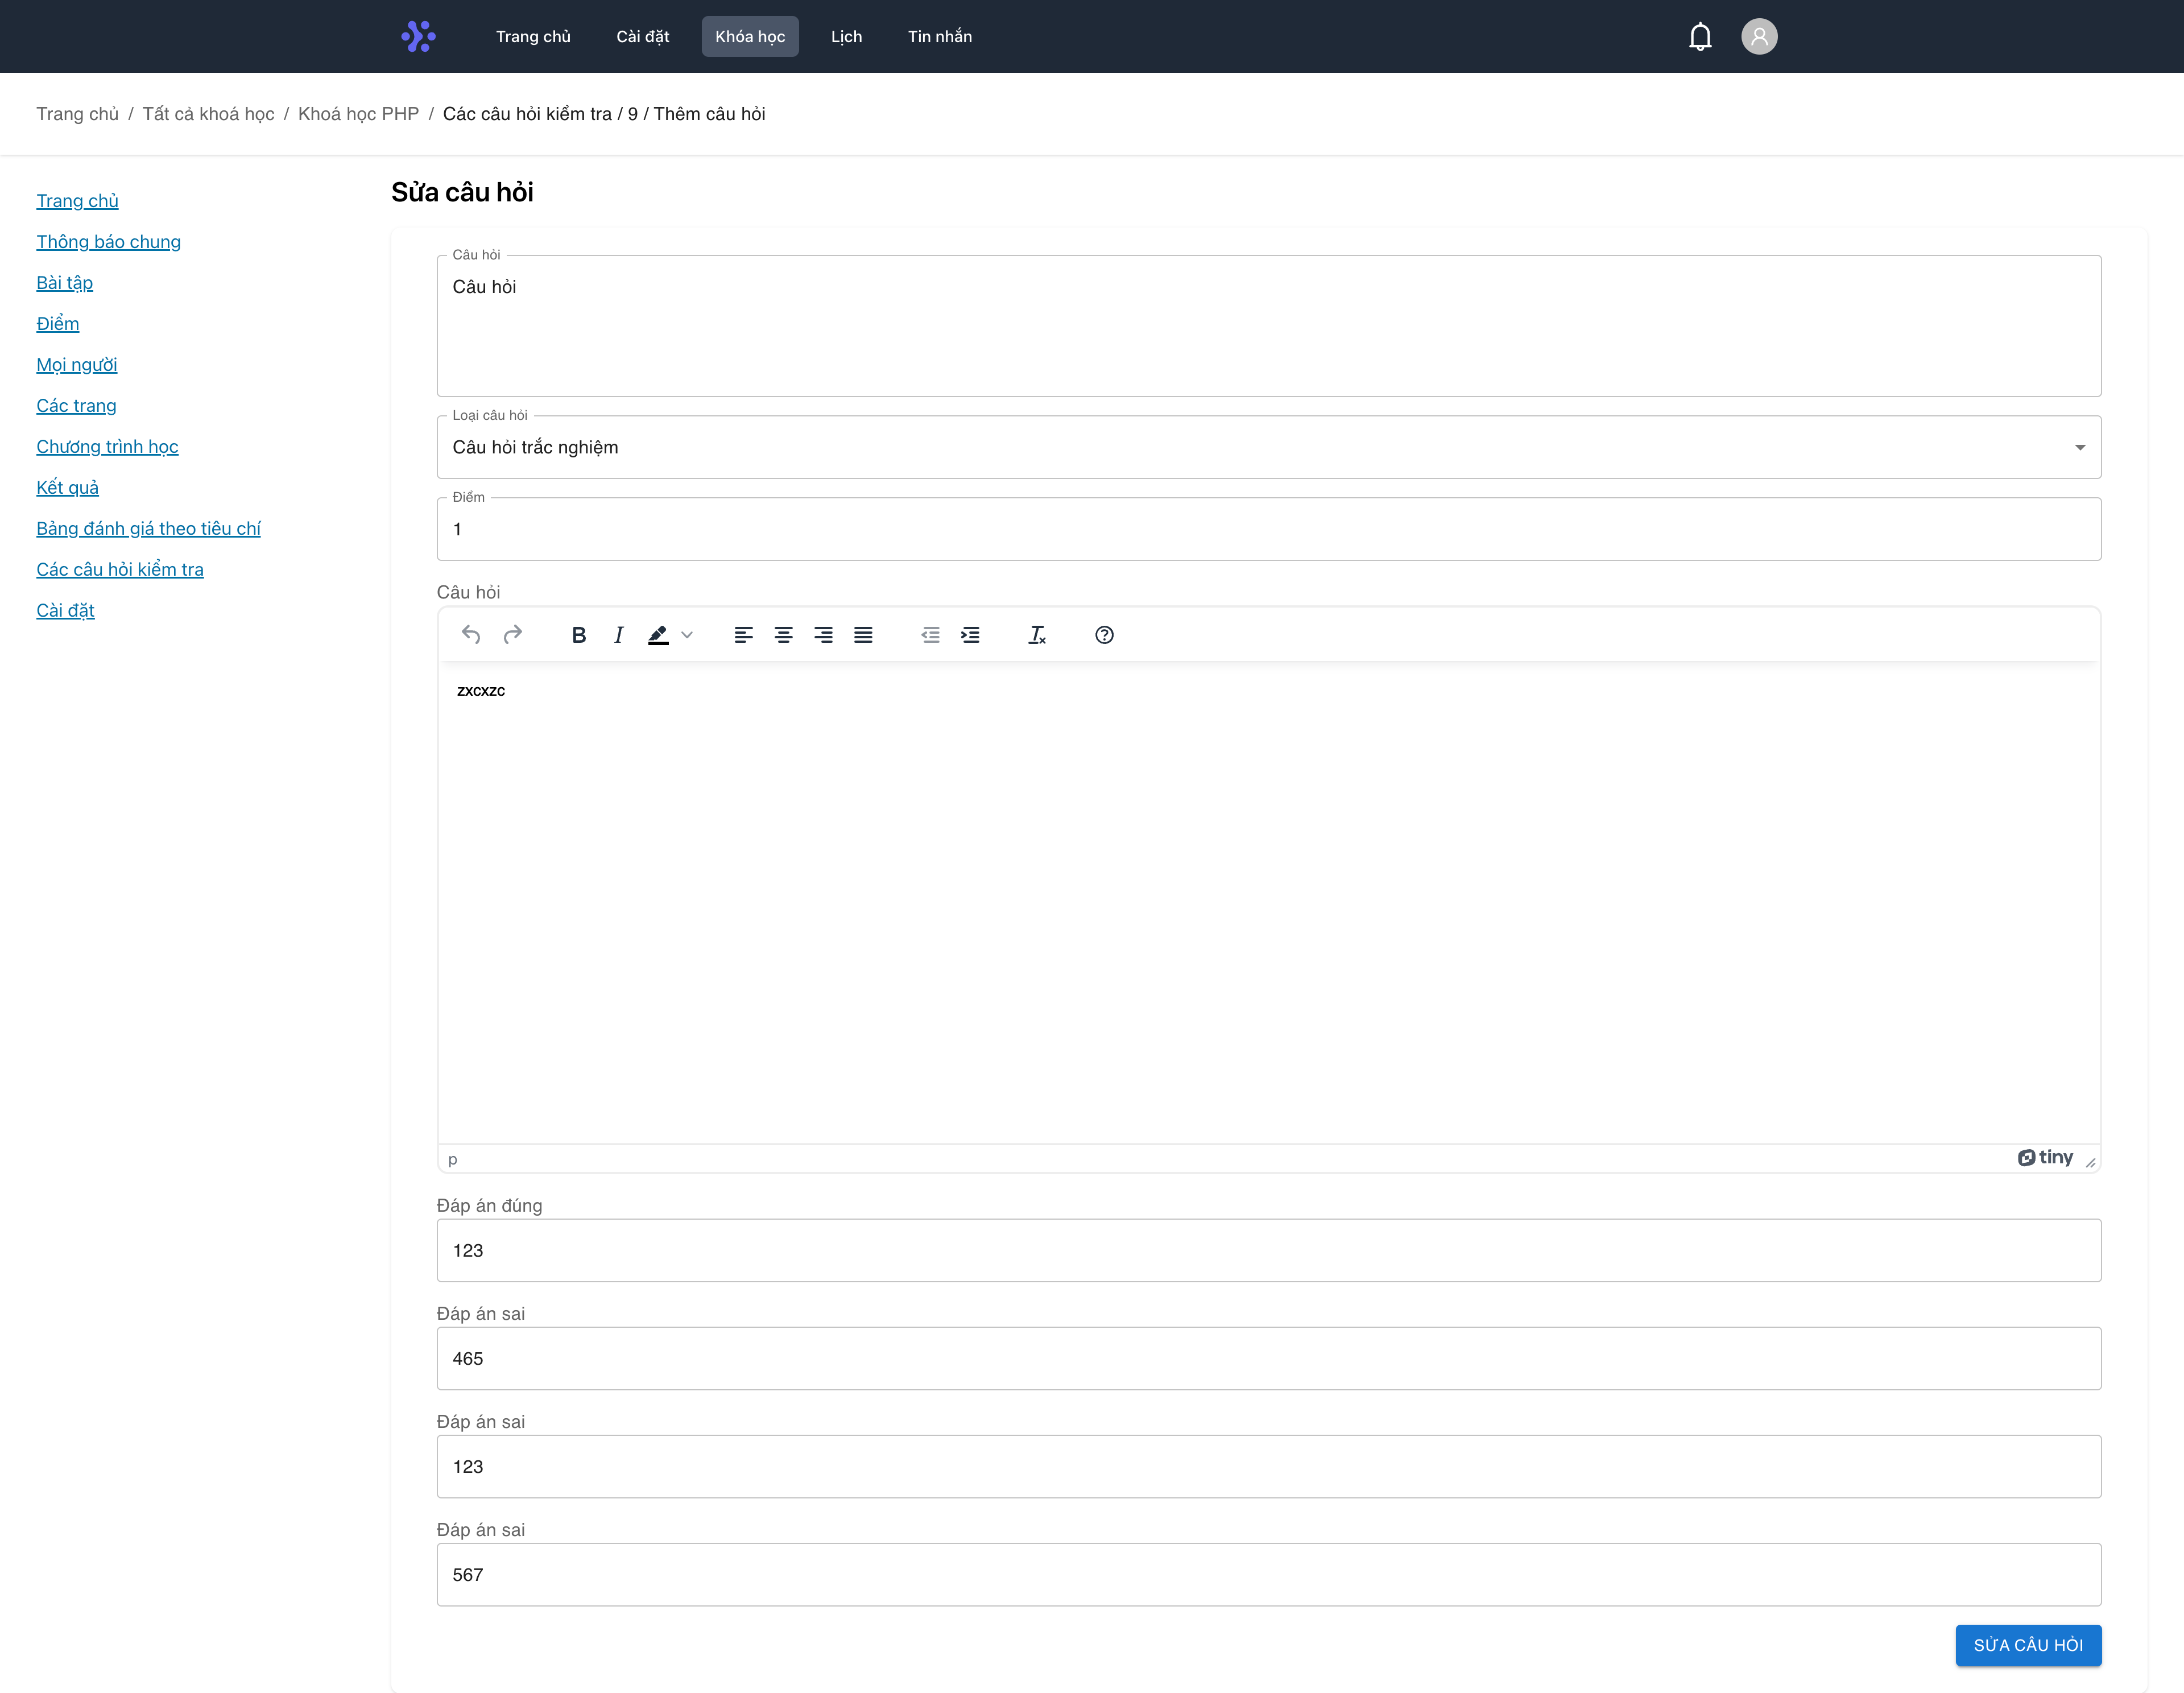
\includegraphics[scale=0.15]{chinh-sua-cau-hoi}
        \caption{Chỉnh sửa câu hỏi}
        \label{fig:chinh-sua-cau-hoi}
    \end{figure}
    

    \begin{figure}[ht!]
        \centering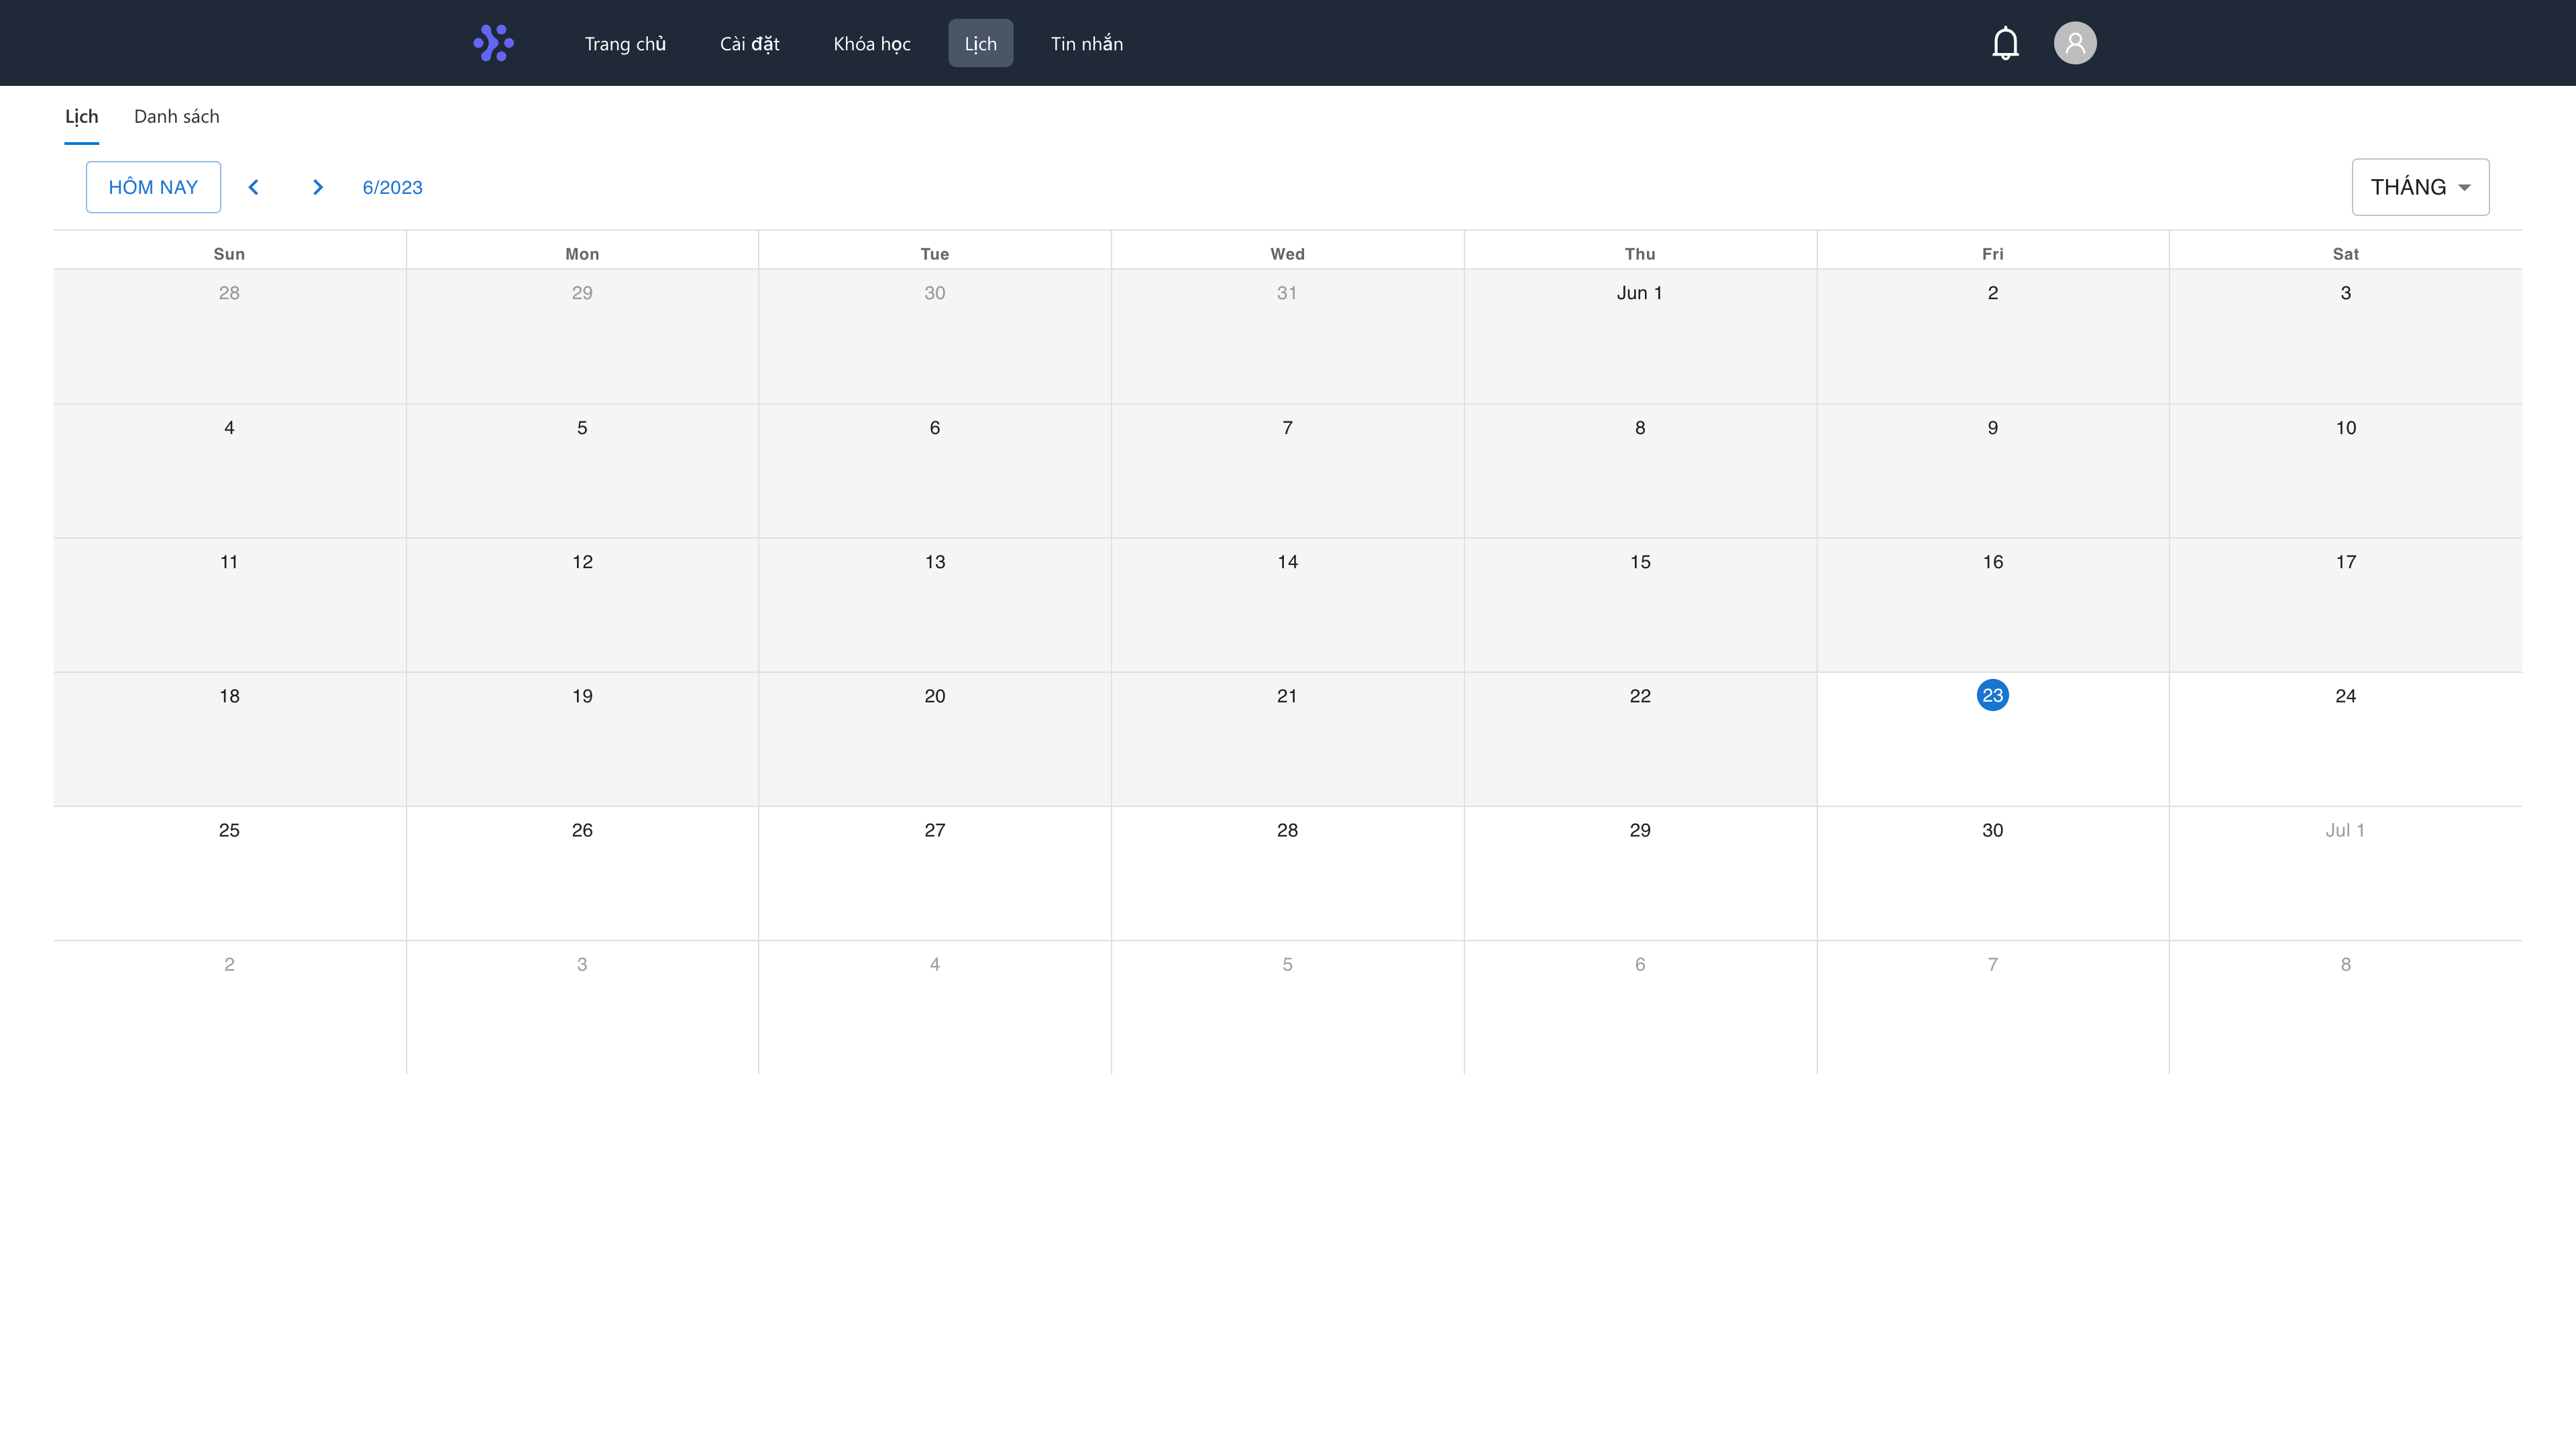
\includegraphics[scale=0.15]{12-lich-su-kien}
        \caption{Màn hình sự kiện dạng lịch}
        \label{fig:lich-su-kien}
    \end{figure}

    \begin{figure}[ht!]
        \centering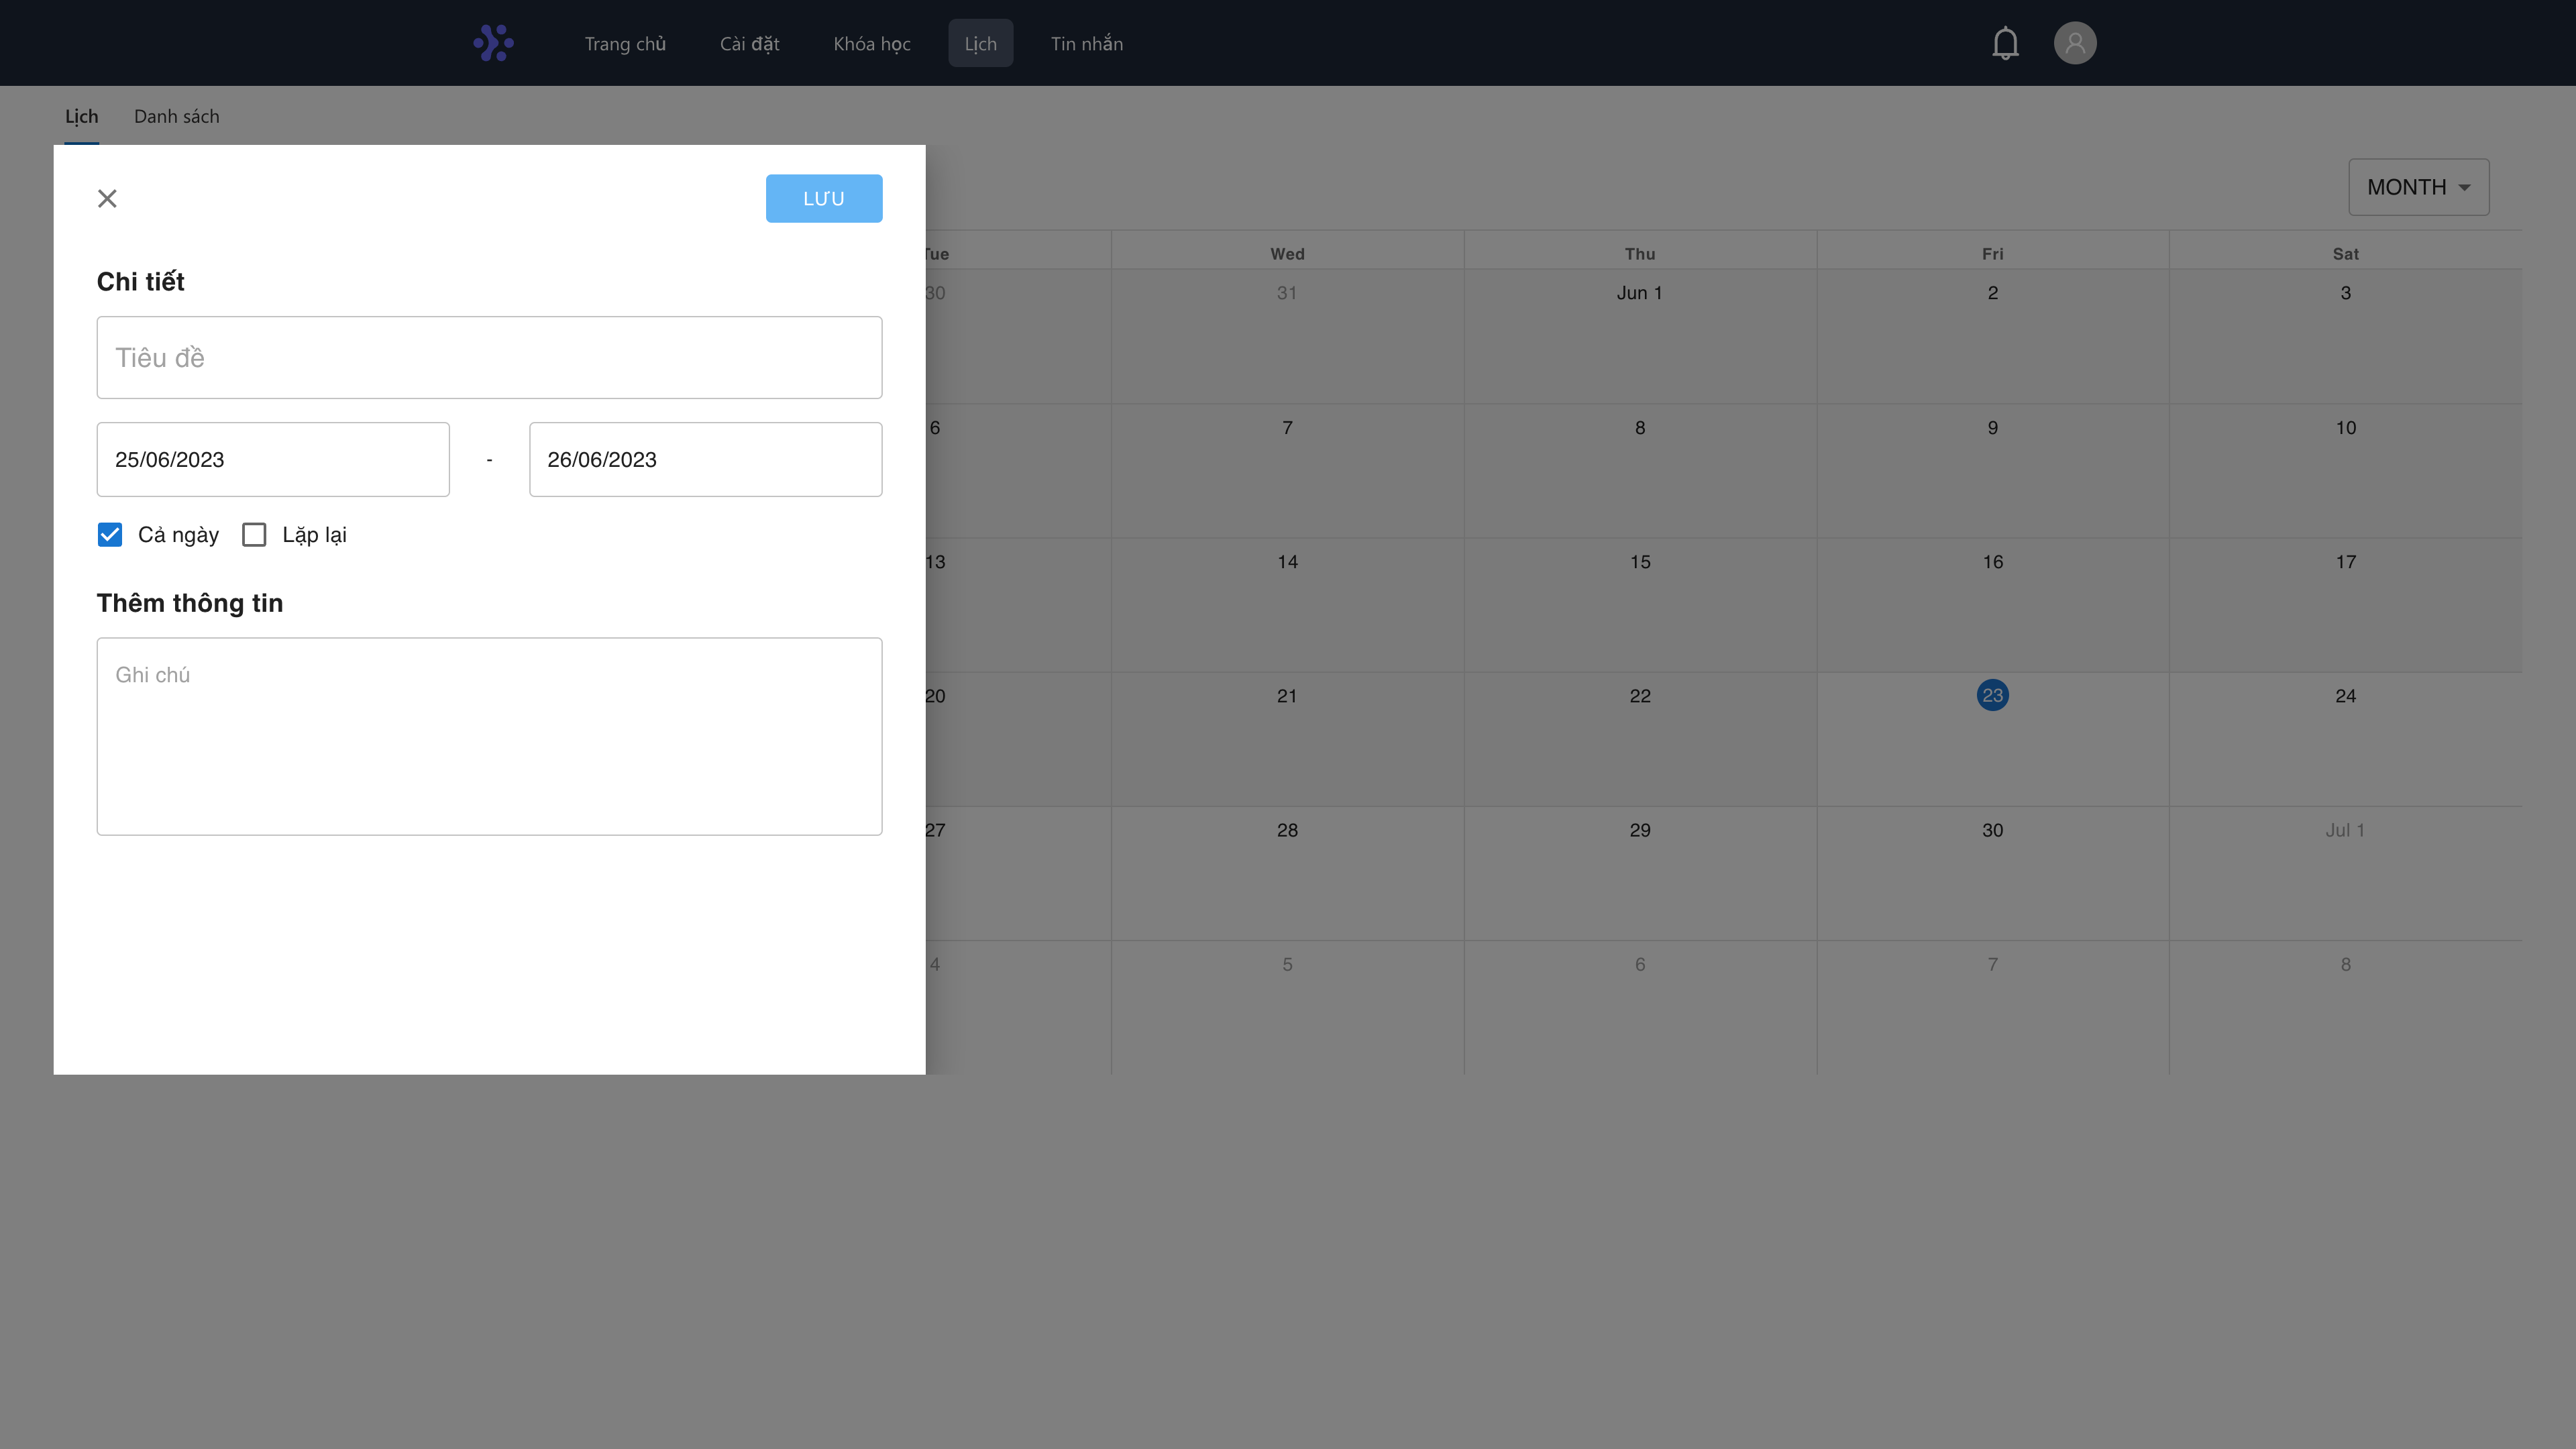
\includegraphics[scale=0.15]{13-tao-su-kien-lich}
        \caption{Màn hình tạo sự kiện}
        \label{fig:thong-bao}
    \end{figure}

    \begin{figure}[ht!]
        \centering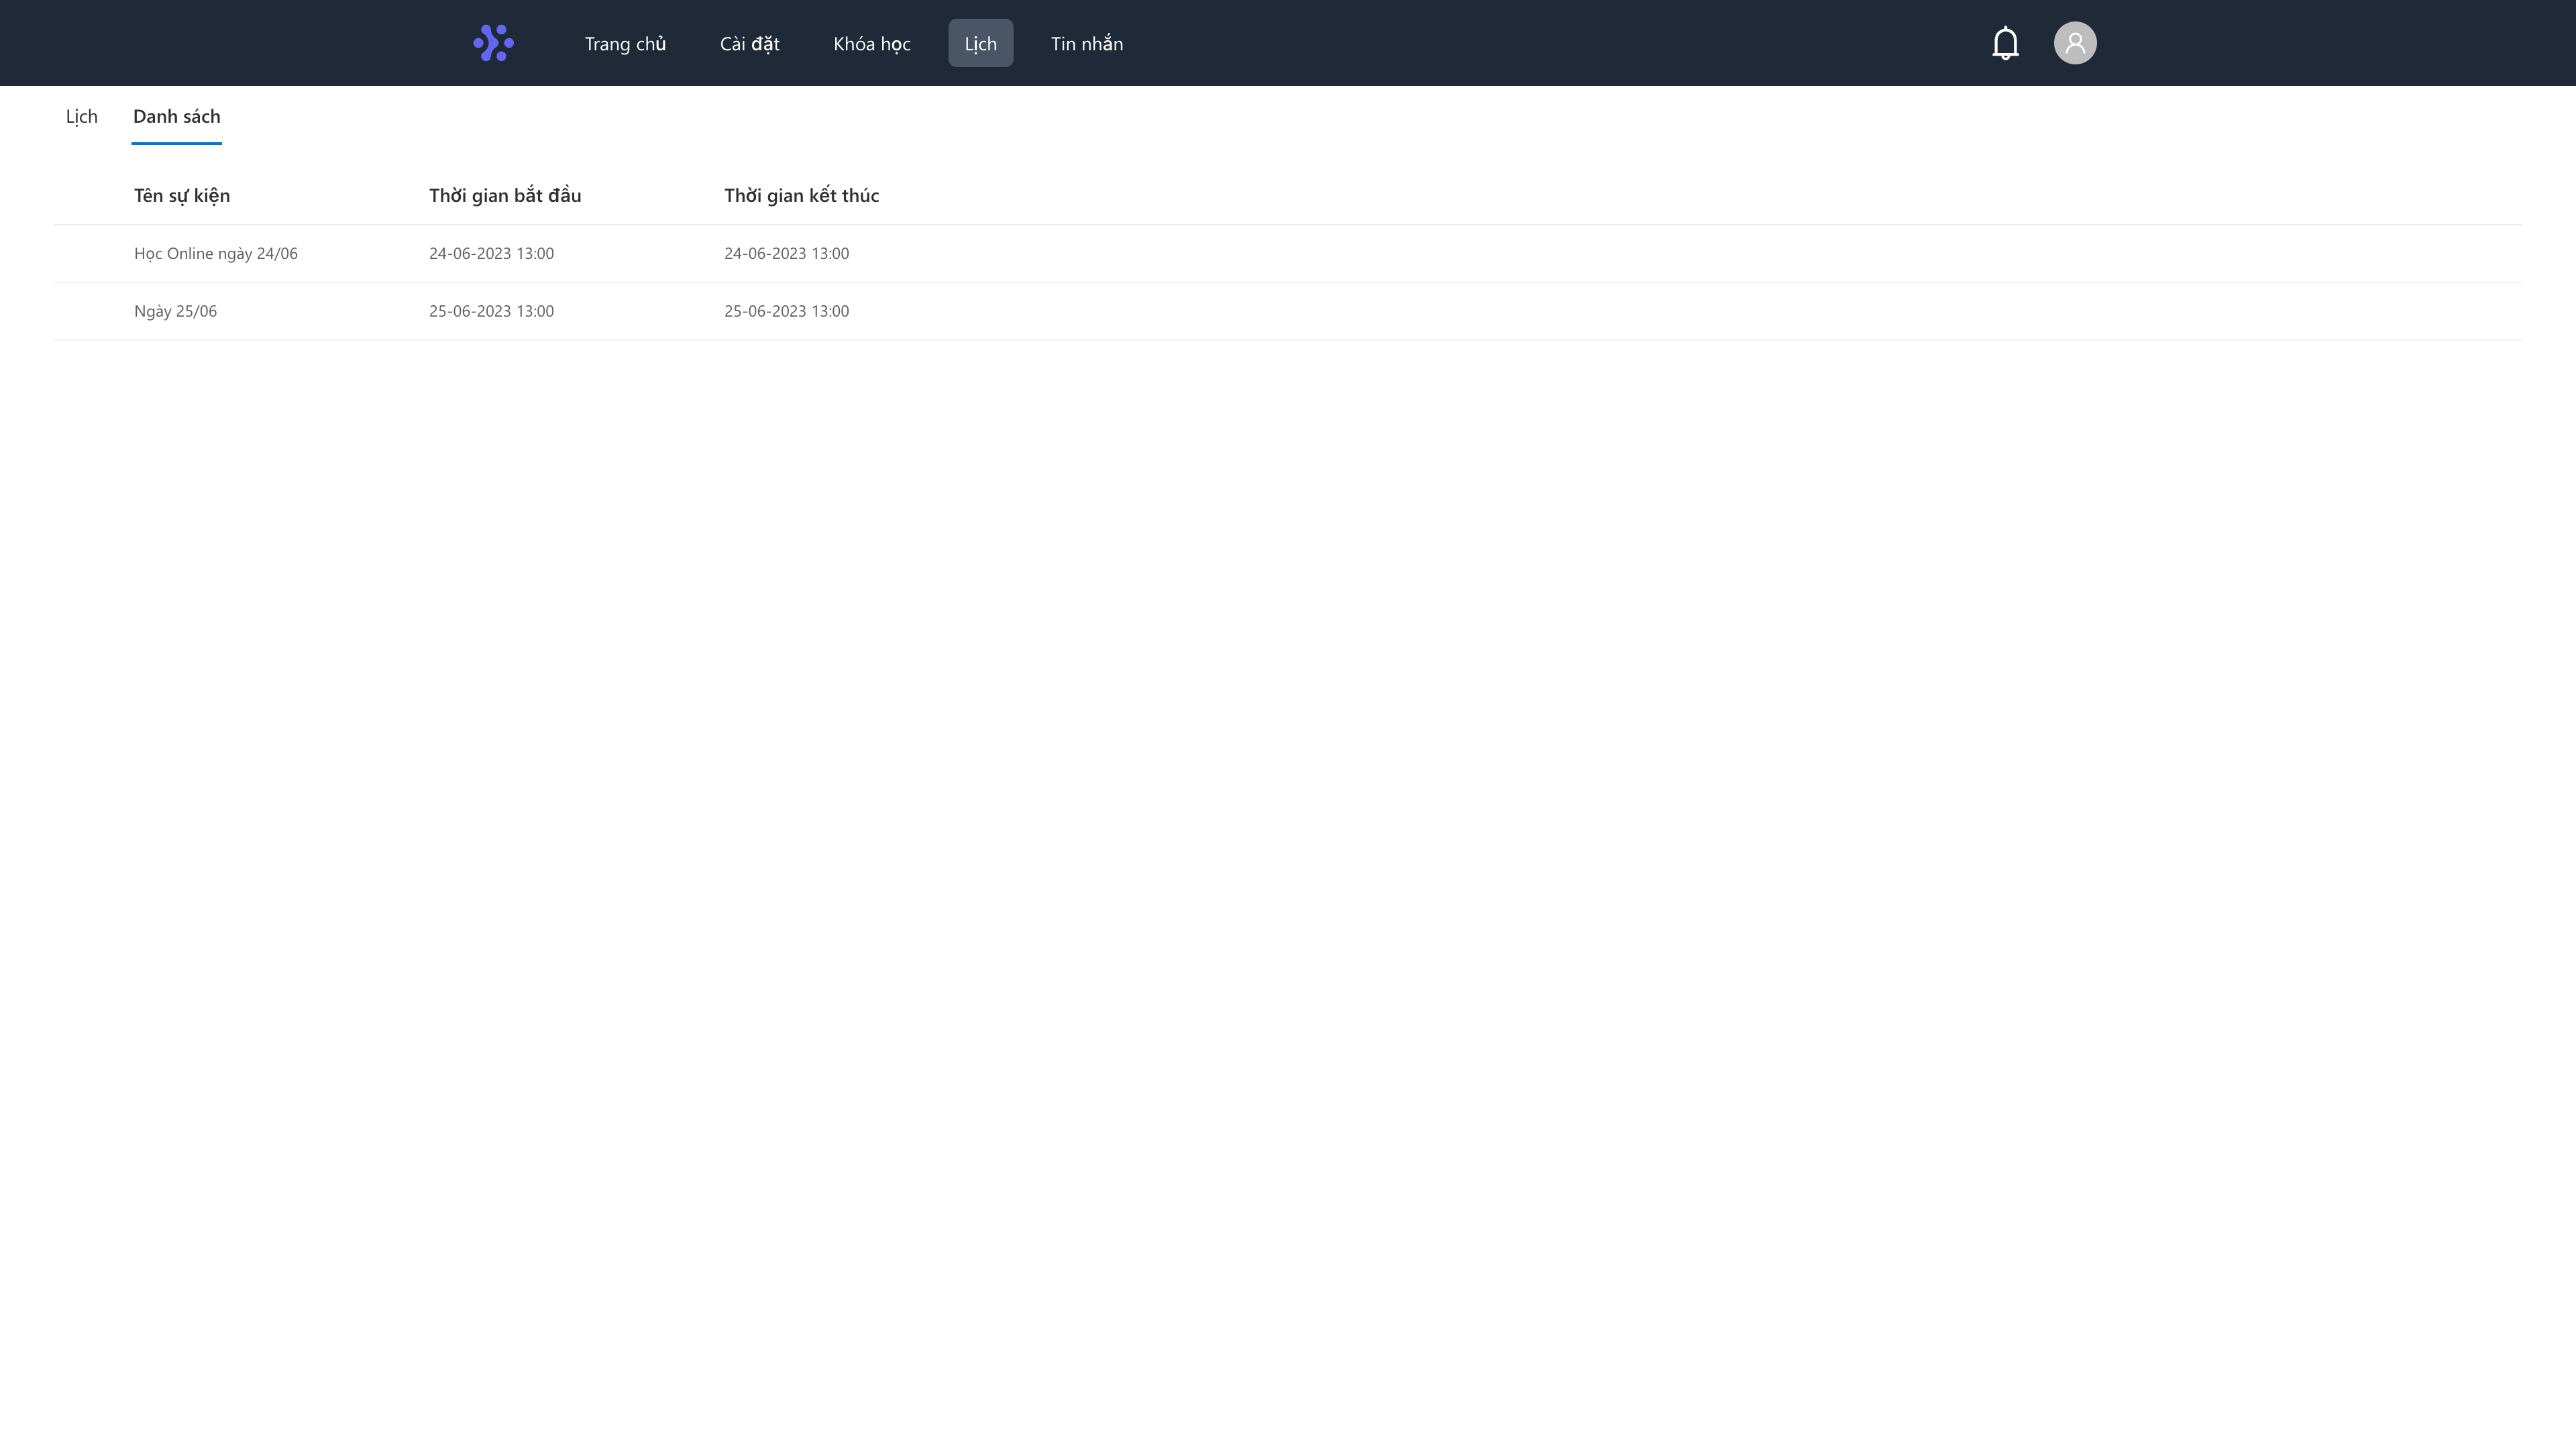
\includegraphics[scale=0.15]{14-danh-sach-su-kien}
        \caption{Màn hình sự kiện dạng danh sách}
        \label{fig:lich-su-kien-danh-sach}
    \end{figure}

    \begin{figure}[ht!]
        \centering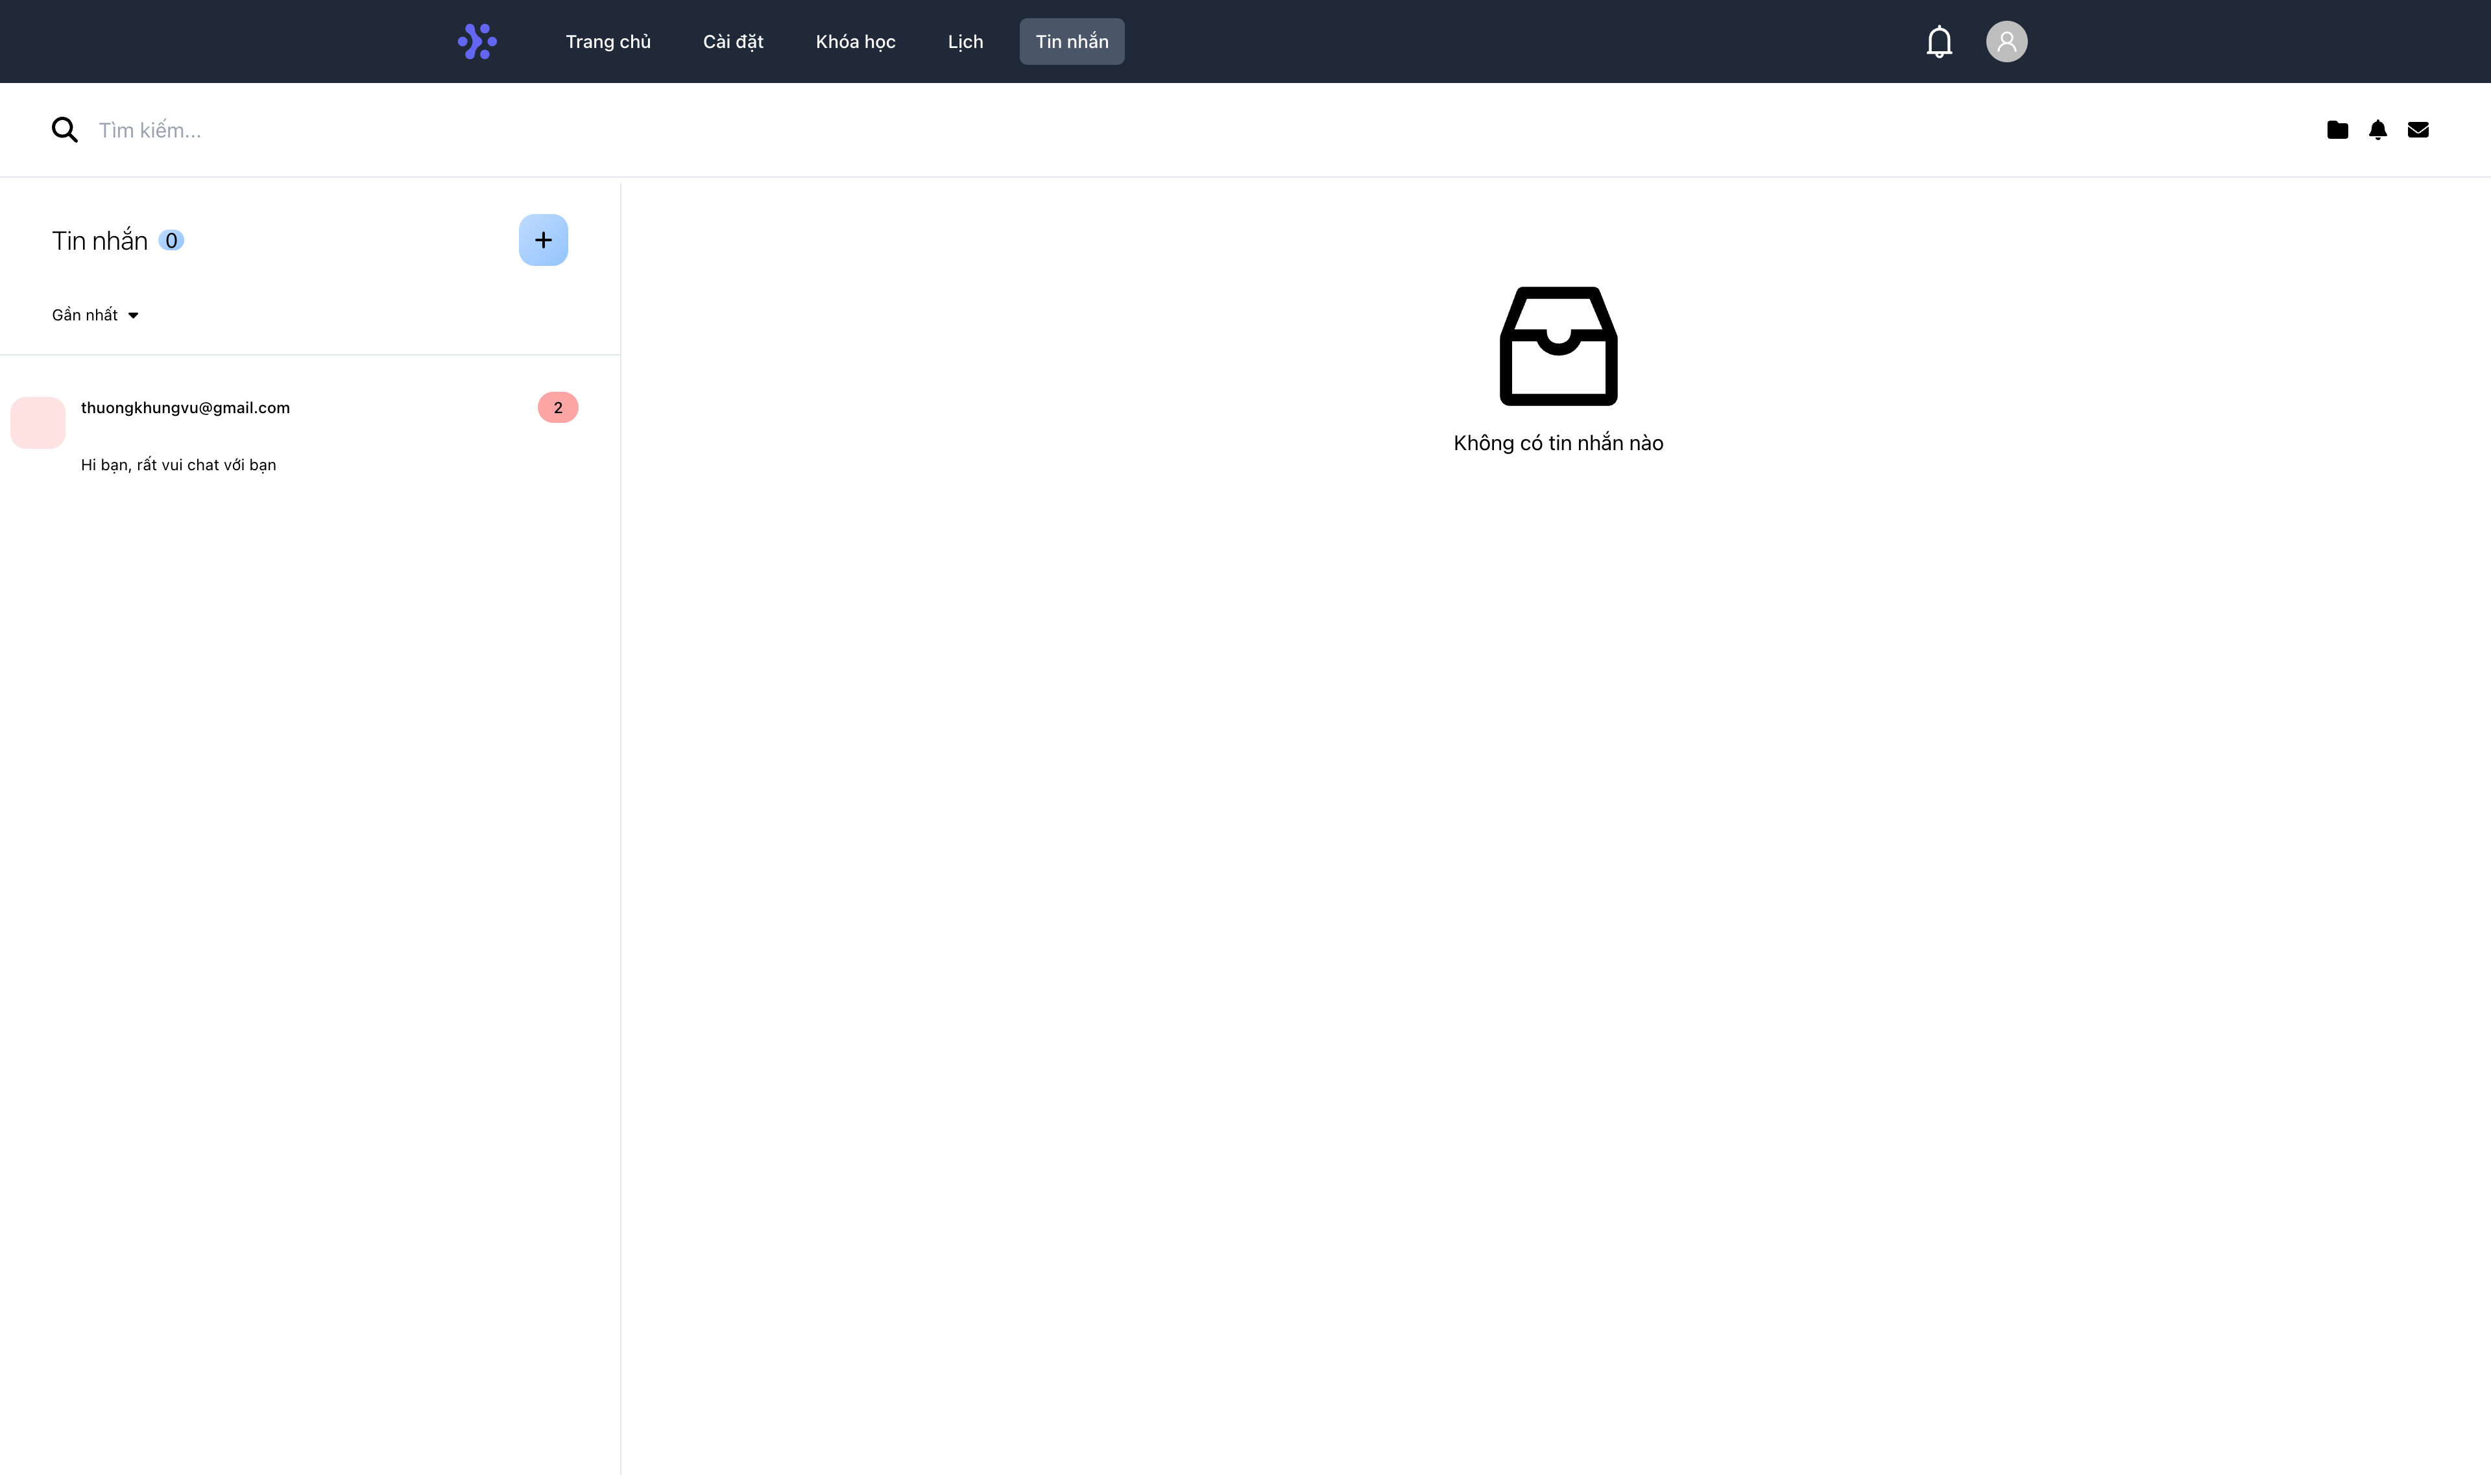
\includegraphics[scale=0.15]{15-tin-nhan}
        \caption{Màn hình danh sách tin nhắn}
        \label{fig:danh-sach-tin-nhan}
    \end{figure}

    \begin{figure}[ht!]
        \centering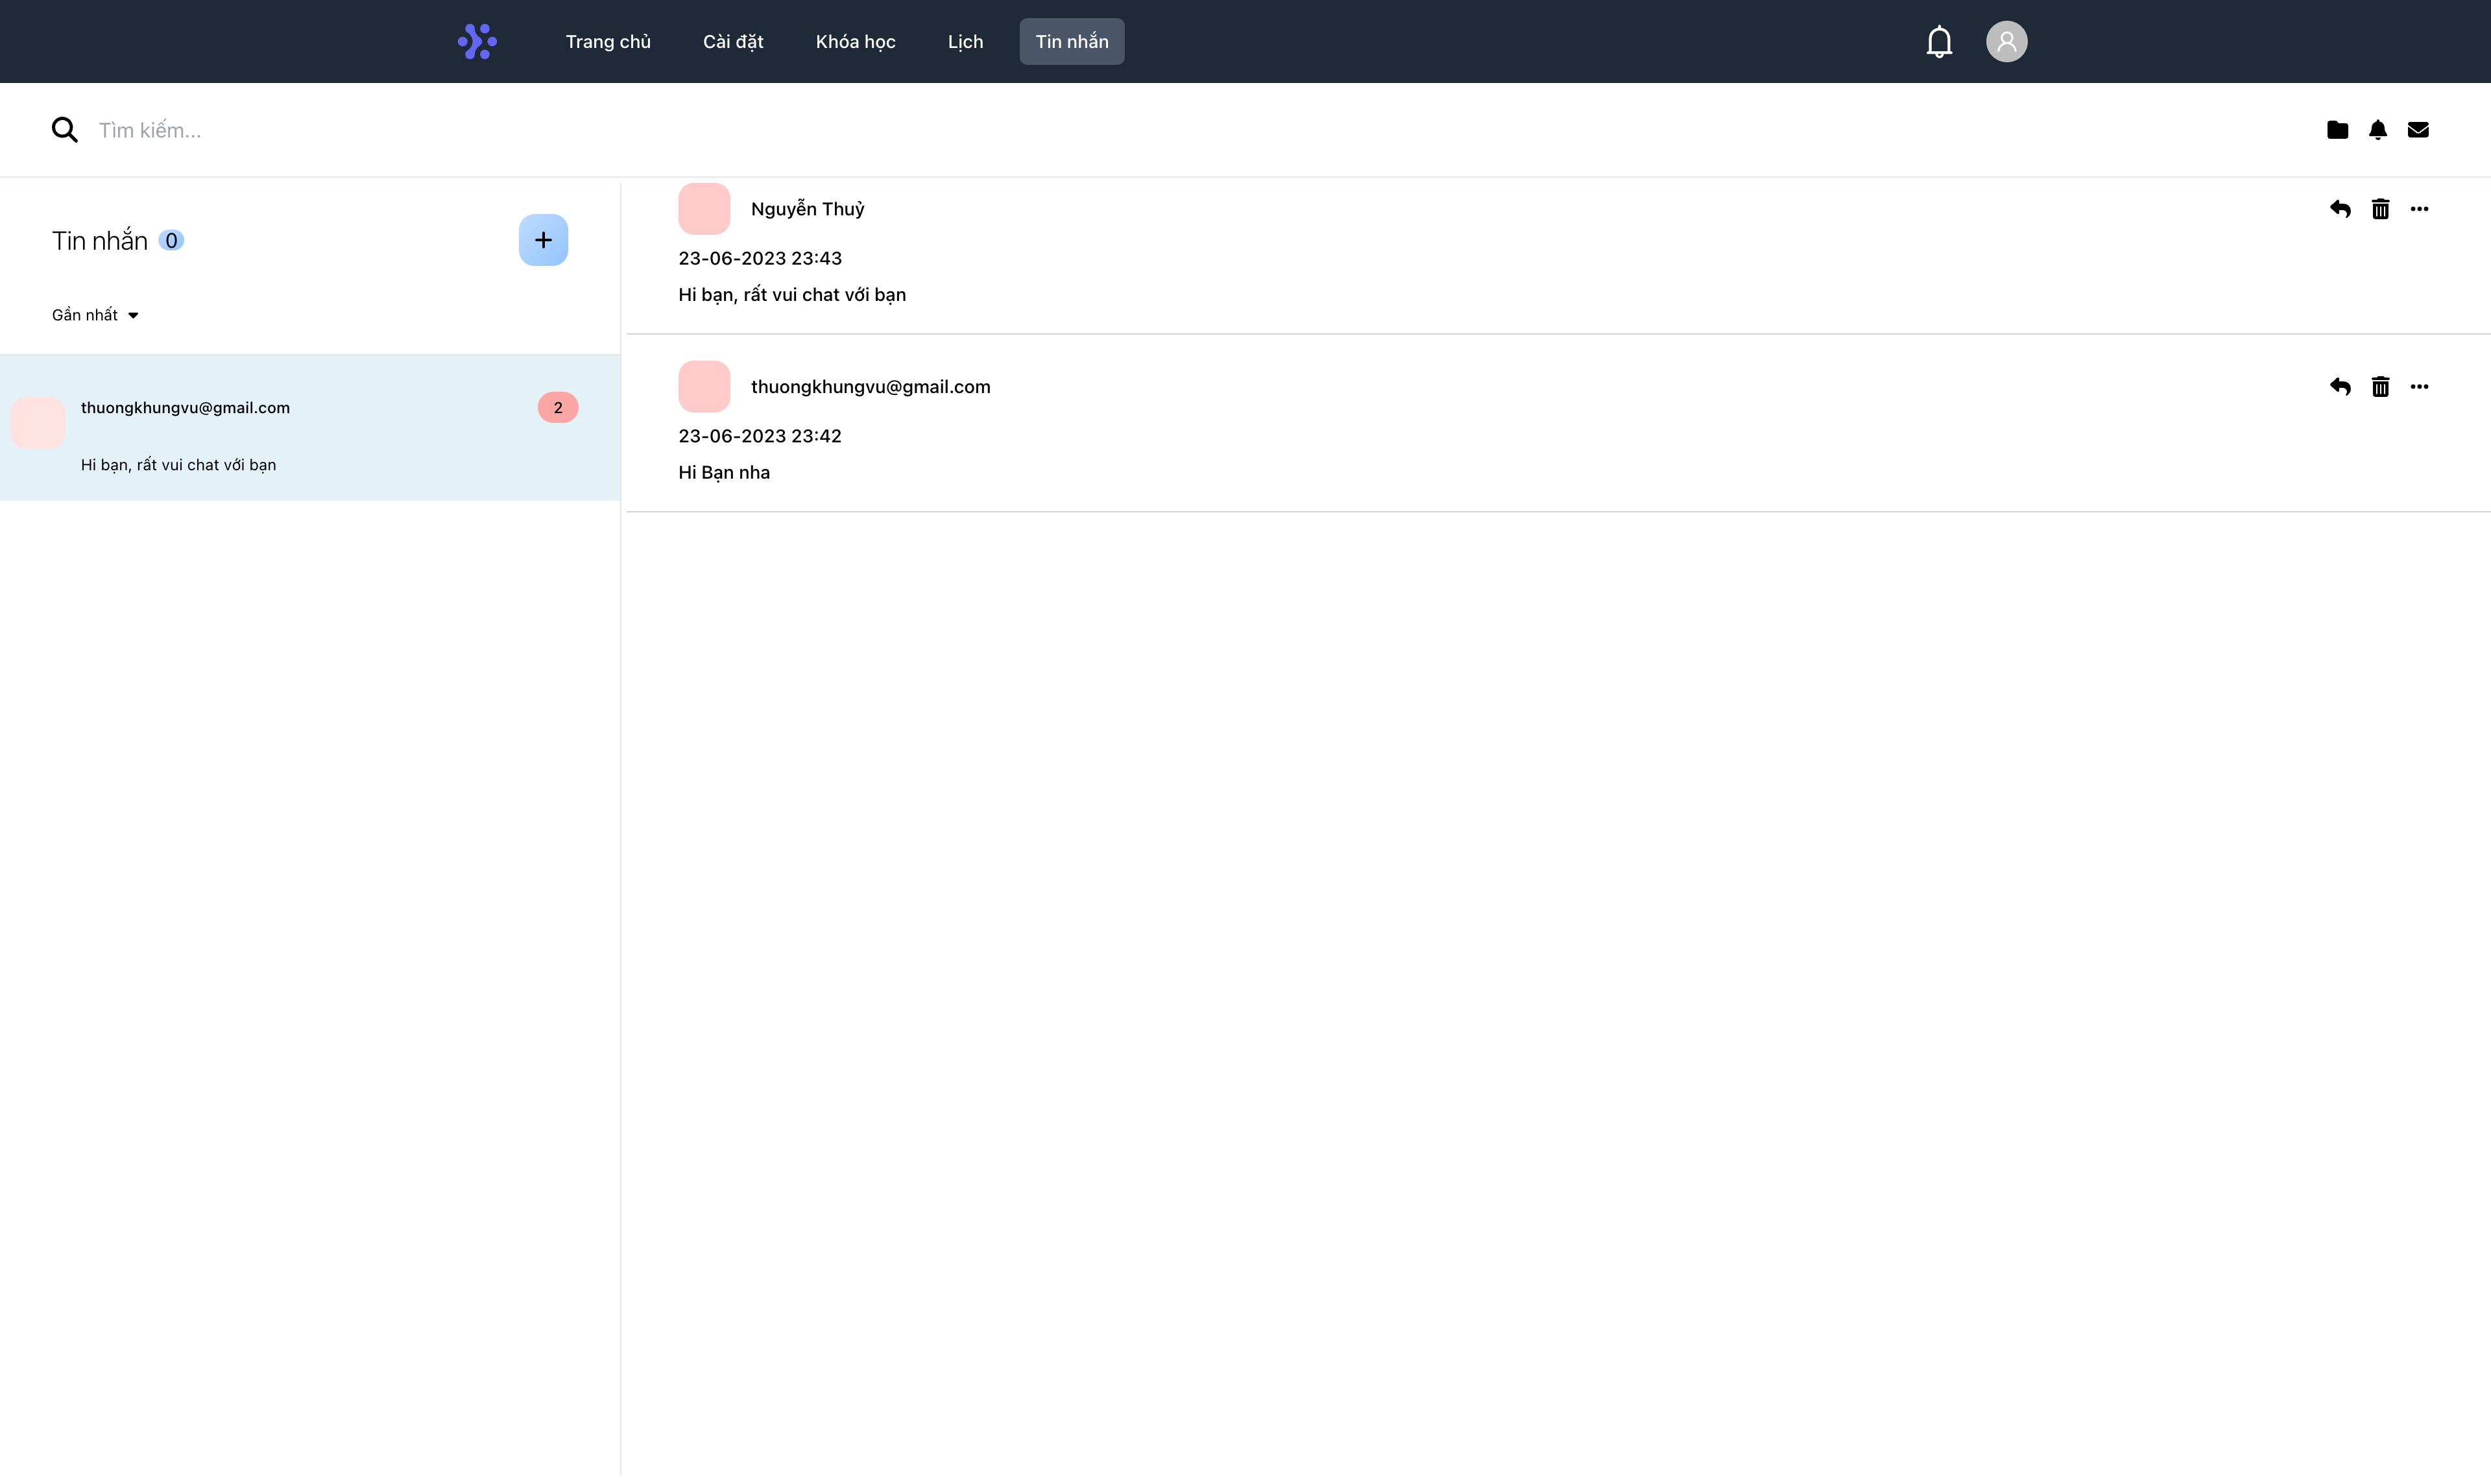
\includegraphics[scale=0.15]{16-chi-tiet-tin-nhan}
        \caption{Màn hình tin nhắn}
        \label{fig:tin-nhan}
    \end{figure}

    \begin{figure}[ht!]
        \centering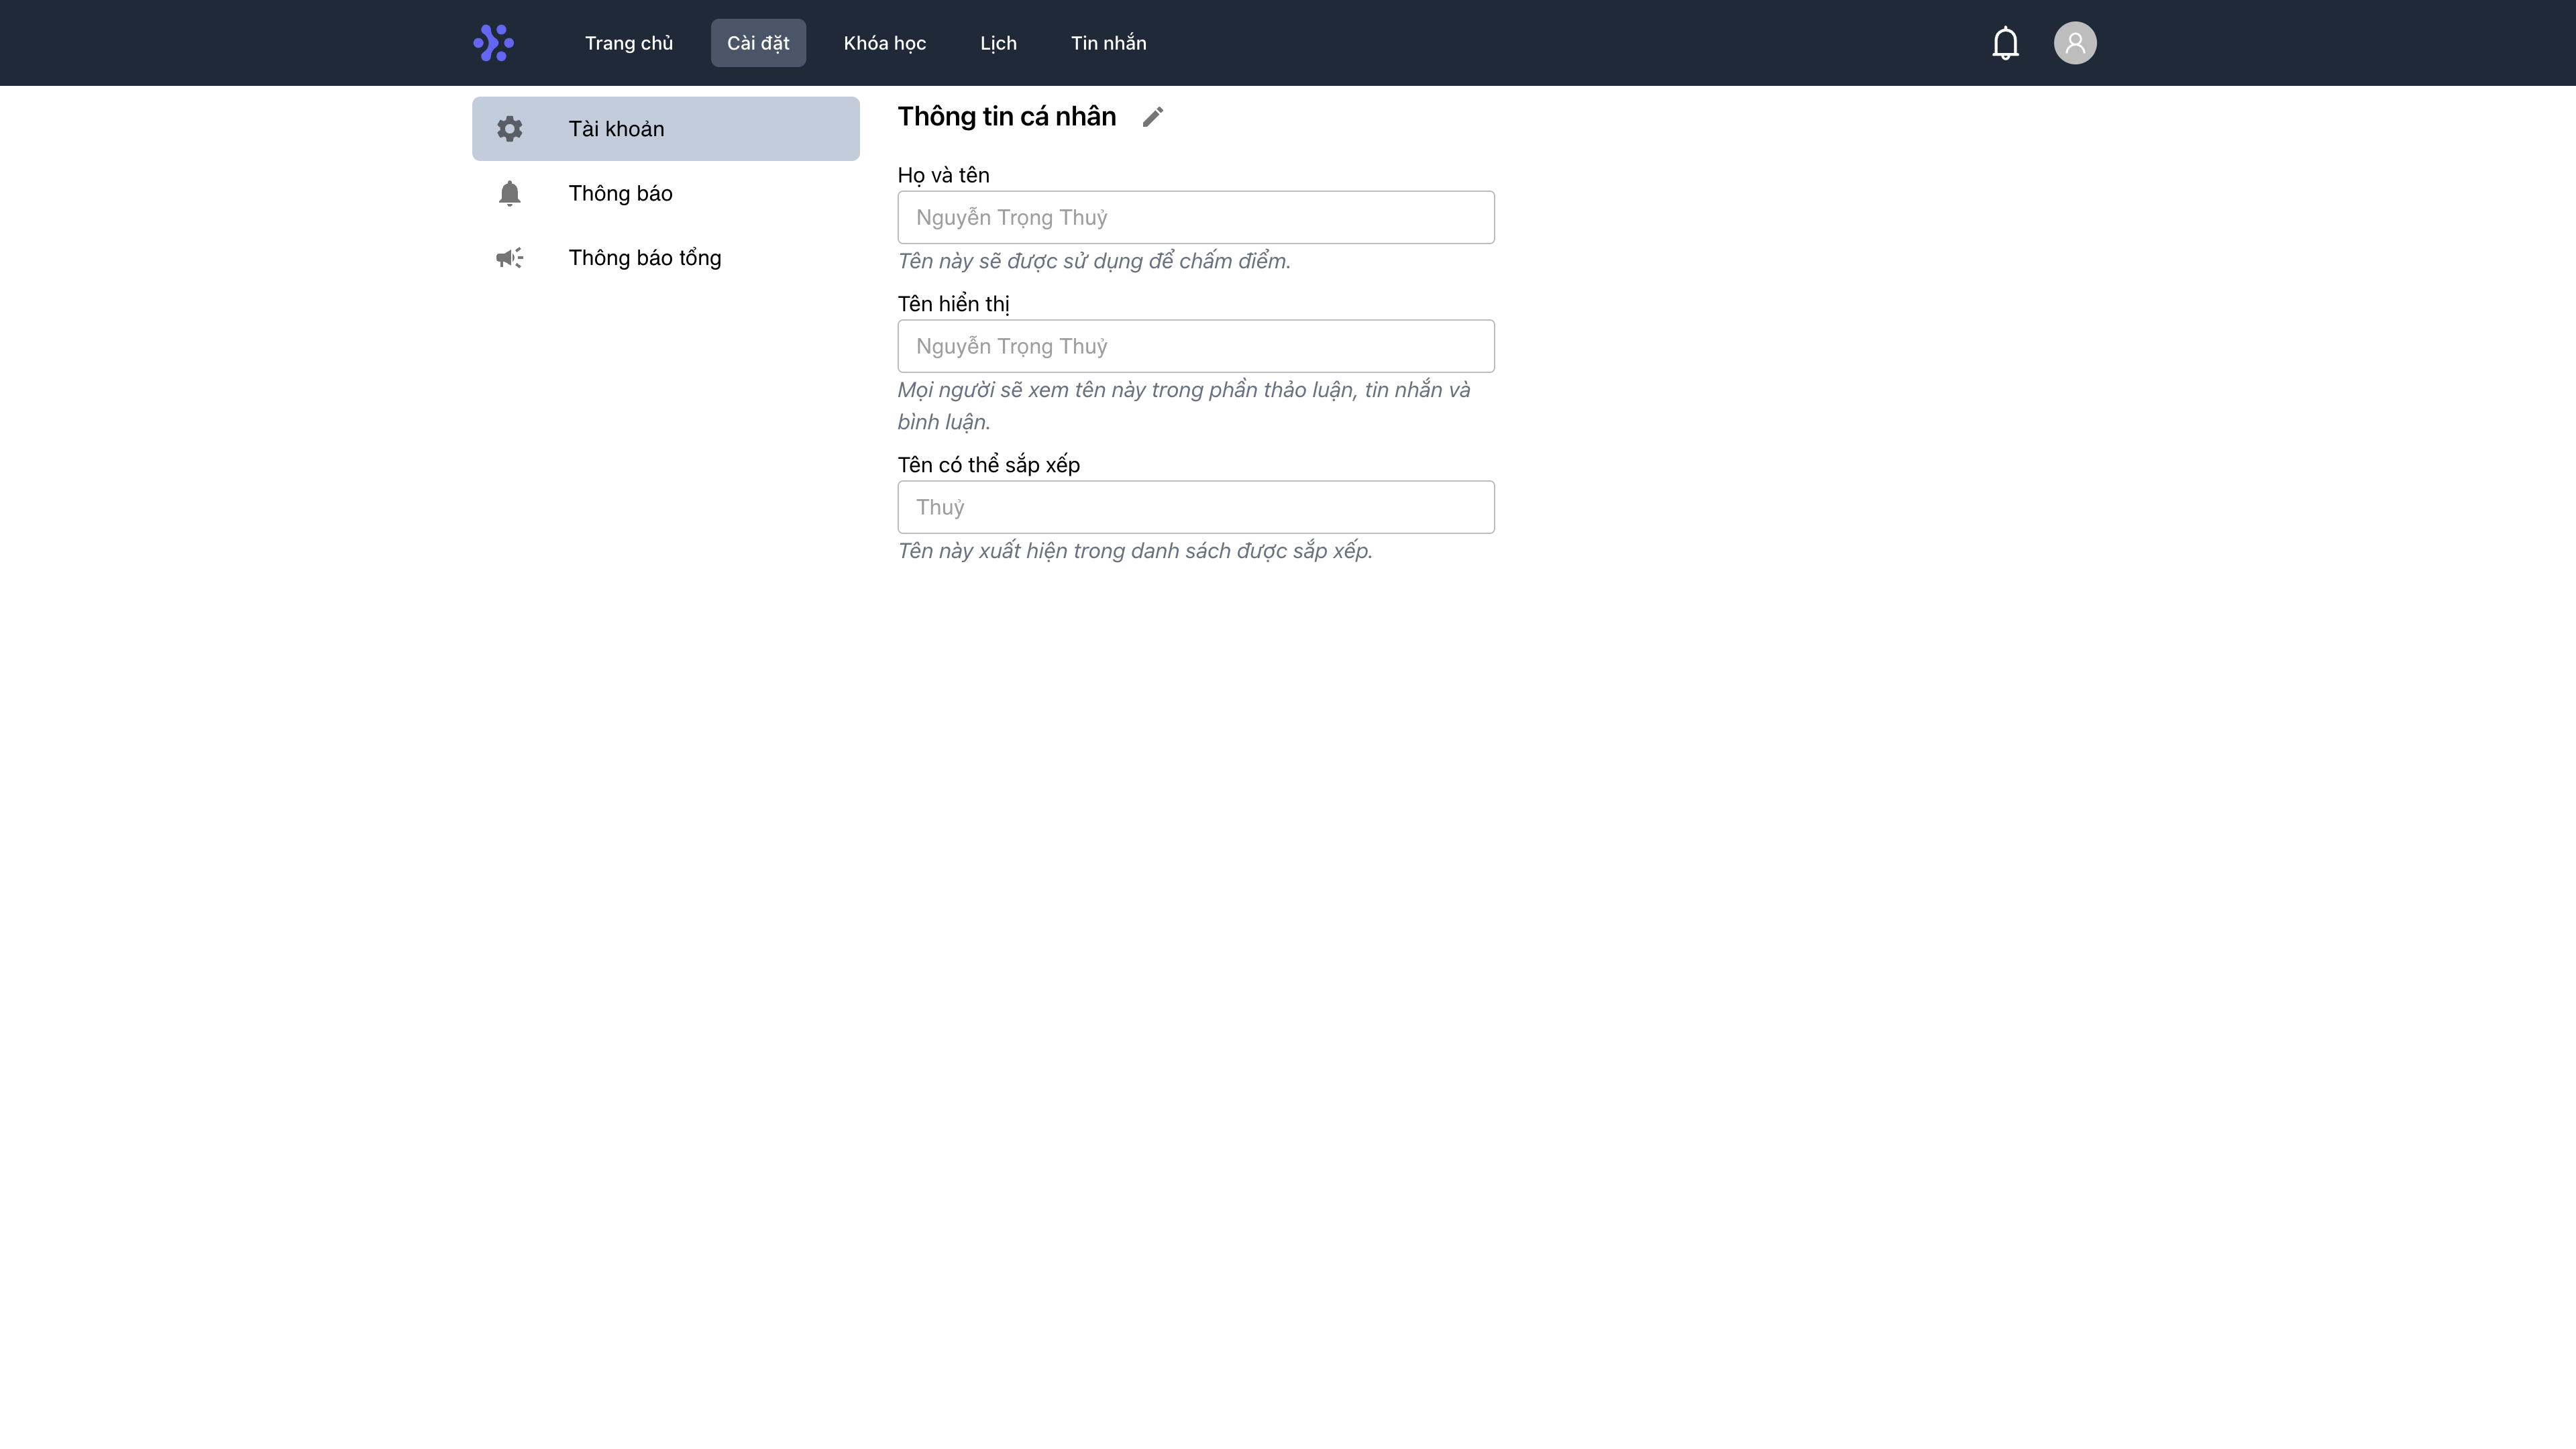
\includegraphics[scale=0.15]{cai-dat}
        \caption{Cài đặt}
        \label{fig:cai-cat}
    \end{figure}

    \begin{figure}[ht!]
        \centering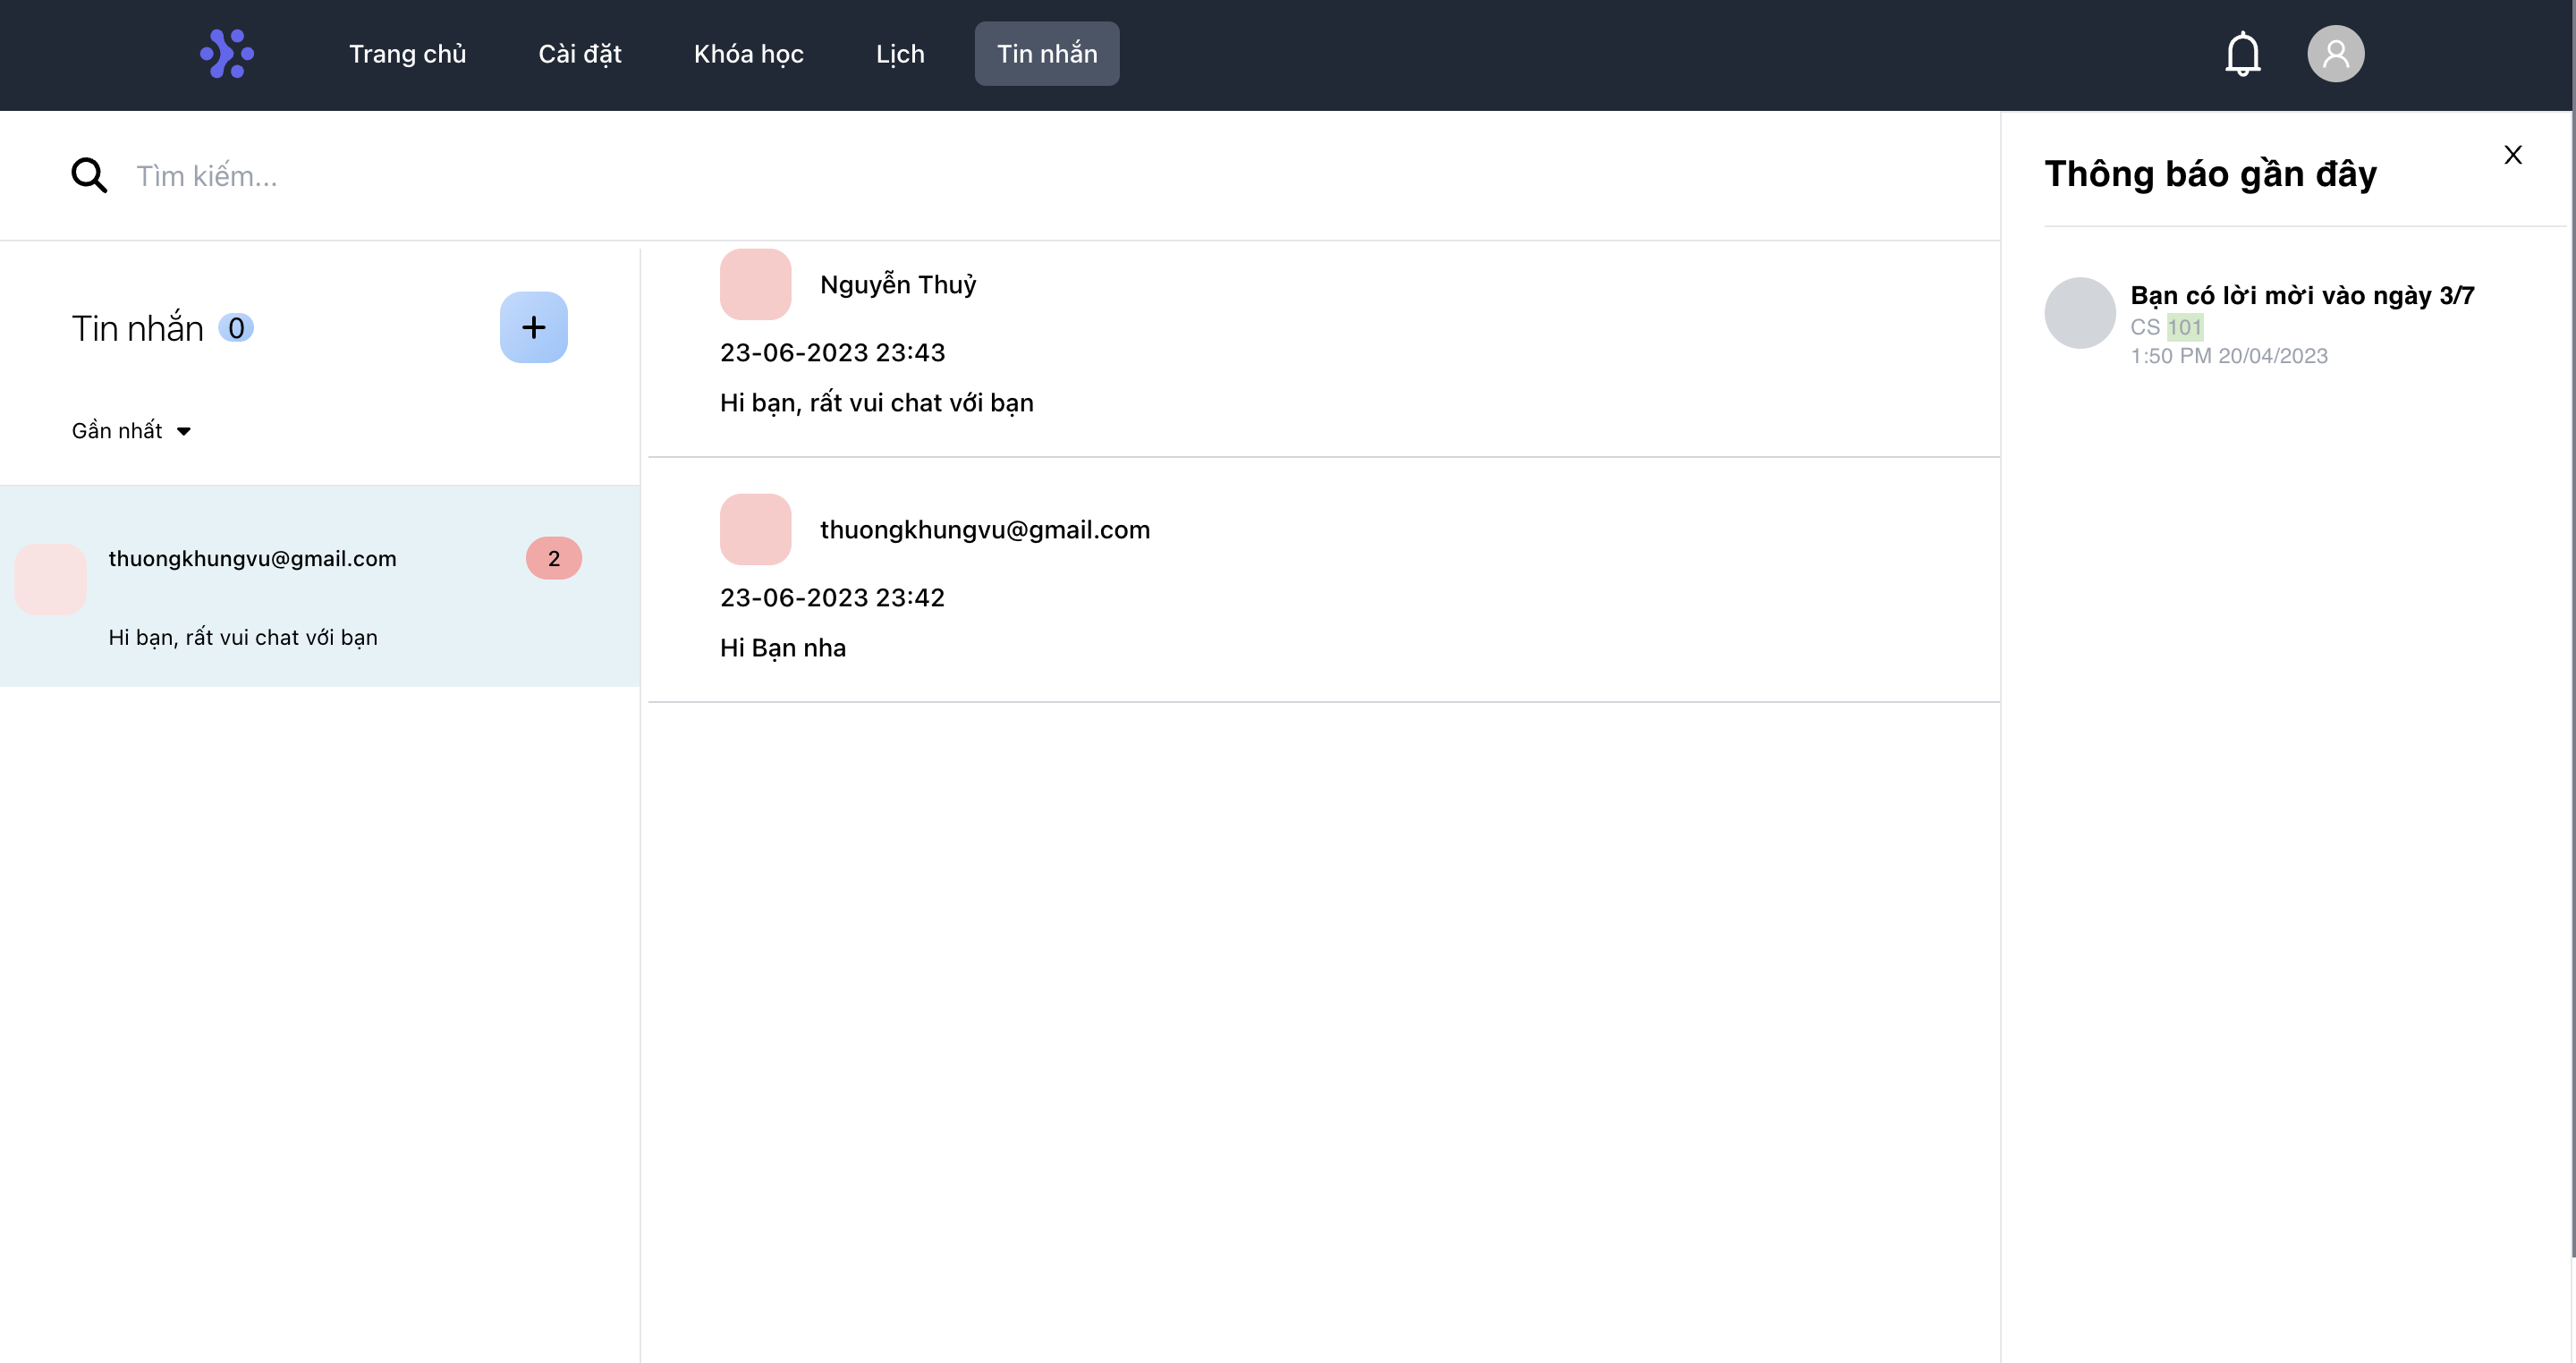
\includegraphics[scale=0.15]{17-thong-bao}
        \caption{Màn hình danh sách thông báo}
        \label{fig:tao-thong-bao}
    \end{figure}


\end{document}